% This is the Reed College LaTeX thesis template. Most of the work
% for the document class was done by Sam Noble (SN), as well as this
% template. Later comments etc. by Ben Salzberg (BTS). Additional
% restructuring and APA support by Jess Youngberg (JY).
% Your comments and suggestions are more than welcome; please email
% them to cus@reed.edu
%
% See http://web.reed.edu/cis/help/latex.html for help. There are a
% great bunch of help pages there, with notes on
% getting started, bibtex, etc. Go there and read it if you're not
% already familiar with LaTeX.
%
% Any line that starts with a percent symbol is a comment.
% They won't show up in the document, and are useful for notes
% to yourself and explaining commands.
% Commenting also removes a line from the document;
% very handy for troubleshooting problems. -BTS

% As far as I know, this follows the requirements laid out in
% the 2002-2003 Senior Handbook. Ask a librarian to check the
% document before binding. -SN

%%
%% Preamble
%%
% \documentclass{<something>} must begin each LaTeX document
\documentclass[12pt,twoside]{reedthesis}
% Packages are extensions to the basic LaTeX functions. Whatever you
% want to typeset, there is probably a package out there for it.
% Chemistry (chemtex), screenplays, you name it.
% Check out CTAN to see: http://www.ctan.org/
%%
\usepackage{graphicx,latexsym}
\usepackage{amsmath}
\usepackage{amssymb,amsthm}
\usepackage{longtable,booktabs,setspace}
\usepackage{chemarr} %% Useful for one reaction arrow, useless if you're not a chem major
\usepackage[hyphens]{url}
% Added by CII
\usepackage{hyperref}
\usepackage{lmodern}
% End of CII addition
\usepackage{rotating}

% Next line commented out by CII
%%% \usepackage{natbib}
% Comment out the natbib line above and uncomment the following two lines to use the new 
% biblatex-chicago style, for Chicago A. Also make some changes at the end where the 
% bibliography is included. 
%\usepackage{biblatex-chicago}
%\bibliography{thesis}


% Added by CII (Thanks, Hadley!)
% Use ref for internal links
\renewcommand{\hyperref}[2][???]{\autoref{#1}}
\def\chapterautorefname{Chapter}
\def\sectionautorefname{Section}
\def\subsectionautorefname{Subsection}
% End of CII addition

% Added by CII 
\usepackage{caption}
\captionsetup{width=5in}
% End of CII addition

% \usepackage{times} % other fonts are available like times, bookman, charter, palatino


% To pass between YAML and LaTeX the dollar signs are added by CII
\title{Enzymatic Promiscuity}
\author{Nelly Selem}
% The month and year that you submit your FINAL draft TO THE LIBRARY (May or December)
\date{Nov 2016}
\division{Mathematics and Natural Sciences}
\advisor{Francisco Barona Gomez}
%If you have two advisors for some reason, you can use the following
% Uncommented out by CII
% End of CII addition

%%% Remember to use the correct department!
\department{Mathematics}
% if you're writing a thesis in an interdisciplinary major,
% uncomment the line below and change the text as appropriate.
% check the Senior Handbook if unsure.
%\thedivisionof{The Established Interdisciplinary Committee for}
% if you want the approval page to say "Approved for the Committee",
% uncomment the next line
%\approvedforthe{Committee}

% Added by CII
%%% Copied from knitr
%% maxwidth is the original width if it's less than linewidth
%% otherwise use linewidth (to make sure the graphics do not exceed the margin)
\makeatletter
\def\maxwidth{ %
  \ifdim\Gin@nat@width>\linewidth
    \linewidth
  \else
    \Gin@nat@width
  \fi
}
\makeatother

\renewcommand{\contentsname}{Table of Contents}
% End of CII addition

\setlength{\parskip}{0pt}

% Added by CII
  %\setlength{\parskip}{\baselineskip}
  \usepackage[parfill]{parskip}

\providecommand{\tightlist}{%
  \setlength{\itemsep}{0pt}\setlength{\parskip}{0pt}}

\Acknowledgements{
I want to thank a few people. Hilda, Cristian, keri, secretaria
inovacion, DNABits
}

\Dedication{
You can have a dedication here if you wish.
}

\Preface{
This is an example of a thesis setup to use the reed thesis document
class.
}

\Abstract{
The preface pretty much says it all. \par  Second paragraph of abstract
starts here.
}

% End of CII addition
%%
%% End Preamble
%%
%

\begin{document}

% Everything below added by CII
      \maketitle
  
  \frontmatter % this stuff will be roman-numbered
  \pagestyle{empty} % this removes page numbers from the frontmatter

      \begin{acknowledgements}
      I want to thank a few people. Hilda, Cristian, keri, secretaria
      inovacion, DNABits
    \end{acknowledgements}
  
      \begin{preface}
      This is an example of a thesis setup to use the reed thesis document
      class.
    \end{preface}
  
      \hypersetup{linkcolor=black}
    \setcounter{tocdepth}{3}
    \tableofcontents
  
      \listoftables
  
      \listoffigures
  
      \begin{abstract}
      The preface pretty much says it all. \par  Second paragraph of abstract
      starts here.
    \end{abstract}
  
      \begin{dedication}
      You can have a dedication here if you wish.
    \end{dedication}
  
  \mainmatter % here the regular arabic numbering starts
  \pagestyle{fancyplain} % turns page numbering back on

  \begin{Shaded}
  \begin{Highlighting}[]
  \CommentTok{# List of packages required for this analysis}
  \NormalTok{pkg <-}\StringTok{ }\KeywordTok{c}\NormalTok{(}\StringTok{"dplyr"}\NormalTok{, }\StringTok{"ggplot2"}\NormalTok{, }\StringTok{"knitr"}\NormalTok{, }\StringTok{"devtools"}\NormalTok{)}
  \CommentTok{# Check if packages are not installed and assign the}
  \CommentTok{# names of the packages not installed to the variable new.pkg}
  \NormalTok{new.pkg <-}\StringTok{ }\NormalTok{pkg[}\OperatorTok{!}\NormalTok{(pkg }\OperatorTok\StringTok{ }\KeywordTok{installed.packages}\NormalTok{())]}
  \CommentTok{# If there are any packages in the list that aren't installed,}
  \CommentTok{# install them}
  \ControlFlowTok{if}\NormalTok{ (}\KeywordTok{length}\NormalTok{(new.pkg))}
    \KeywordTok{install.packages}\NormalTok{(new.pkg, }\DataTypeTok{repos =} \StringTok{"http://cran.rstudio.com"}\NormalTok{)}
  \CommentTok{# Load packages}
  \KeywordTok{library}\NormalTok{(dplyr)}
  \KeywordTok{library}\NormalTok{(ggplot2)}
  \KeywordTok{library}\NormalTok{(knitr)}
  \end{Highlighting}
  \end{Shaded}
  
  \chapter{EvoMining}\label{rmd-basics}
  
  \section{Introduction}\label{introduction}
  
  Enzyme promiscuity on metabolic families, can be looked on enzymes that
  are over a divergent process.
  
  \section{Gen families expansions on
  genomes}\label{gen-families-expansions-on-genomes}
  
  \subsection{Pangenomes}\label{pangenomes}
  
  Expansions are located on pangenome, Tools to analyse pangenome BPgA
  
  \section{EvoMining}\label{evomining}
  
  EvoMining looks expansions on prokariotic pangenome.\\
  Biological idea.
  
  EvoMining was available as a consult website with 230 members of the
  Actinobacteria phylum as genomic data base, 226 unclassified nBGCs, and
  not interchangable central database 339 queries for nine pathways,
  including amino acid biosynthesis, glycolysis, pentose phosphate
  pathway, and tricarboxylic acids cycle.
  {[}\protect\hyperlink{ref-cruz-morales_phylogenomic_2016}{1}{]}
  EvoMining was proved on Actinobacteria Arseno-lipids
  
  \section{Pangenome}\label{pangenome}
  
  The sequenced genome of an individull in some species is just a partil
  print of the species geneticll repertoire Individualls can gain and loss
  genes.\\
  {[}\protect\hyperlink{ref-koonin_turbulent_2015}{2}{]} Pangenome is the
  total sequenced gene pool in a taxonomically related group. Supergenome
  all the possible extant genes. About 10 times genomes. there are open,
  closed pangenomes.Most genomes has a core a shell and a unique genes.\\
  Gene history its a tree history
  
  HGT doubles mutation rate on prokarites.\\
  Maybe HGT is an selected feature, if is the case, so could be np
  production.\\
  Some archaeas has open pangenome.
  {[}\protect\hyperlink{ref-halachev_calculating_2011}{3}{]}
  
  HGT doubles mutation rate on prokarites.
  {[}\protect\hyperlink{ref-koonin_turbulent_2015}{2}{]} Maybe HGT is an
  selected feature, if is the case, so could be np production.\\
  Some archaeas has open pangenome.
  {[}\protect\hyperlink{ref-halachev_calculating_2011}{3}{]} Shell trees
  converge to core trees
  {[}\protect\hyperlink{ref-narechania_random_2012}{4}{]}
  
  \section{EvoMining Implementation}\label{evomining-implementation}
  
  \textbf{EvoMining} was expanded from a website
  (\url{http://evodivmet.langebio.cinvestav.mx/EvoMining/index.html}) with
  limited datasets to an easy to install distribution that allows
  flexiblibilty on genomic, central and natural product databases.
  Evomining user distribution was developed on perl on Ubuntu-14.04 but
  wraped on \href{https://www.docker.com/}{Docker}. Docker is a software
  containerization platform that allows repetibilty regardless of the
  environment. Docker engine is avilable for Linux, Cloud, macOS 10.10.3
  Yosemite or newer and even 64bit Windows 10.
  
  Dependencies that were packaged at EvoMining docker app are Apache2,
  muscle3.8.31, newick-utils-1.6,quicktree, blast-2.2.30,
  Gblocks\_Linux64\_0.91b perl and from cpan CGI, SVG and
  Statistics::Basic modules.
  
  Github defines itself as an online project hosting using Git. Its free
  for open source-code hosting and facilitates team work. Includes
  source-code browser, in-line editing, and wikis.
  
  Dockerhub is an apps project hosting.
  
  \href{https://hub.docker.com/u/nselem/}{Dockerhub nselem}
  
  EvoMining code is open source and it is available at a github repository
  \href{https://github.com/nselem/EvoMining}{github/EvoMining}
  
  Github and Dockerhub can be coneccted by the use of repositories
  automatically built. Among the advantages of automated builds are that
  the DockerHub repository is automatically kept up-to-date with code
  changes on GitHub and that its Dockerfile is available to anyone with
  access to the Docker Hub repository. EvoMining is stored on a DockerHub
  automated build repository linked to github EvoMining repository so that
  code is always actualized.
  
  To download EvoMining image from docker Hub once Docker engine is
  installed its necessary to run the following command at a terminal:\\
  \texttt{docker\ pull\ nselem/newevomining}
  
  To run EvoMining container\\
  \texttt{docker\ run-i\ -t\ \ -v\ /home/nelly/docker-evomining:/var/www/html\ -p\ 80:80\ evomining\ /bin/bash}
  
  To start evoMining app \texttt{perl\ startEvomining}\\
  `` Detailed tutorial, EvoMining description, pipeline and user guide are
  available at a wiki on github at
  \href{https://github.com/nselem/EvoMining/wiki}{EvoMining wiki}.
  
  Other genomic apps were containerized to docker images during this
  work.\\
  - \emph{myRAST} docker- \url{https://github.com/nselem/myrast}\\
  RAST is a bacterial and Archaeal genome annotator
  {[}\protect\hyperlink{ref-aziz_rast_2008}{5}{]} This app allows myRAST
  functionality to upload\\
  It allows EvoMining genome database annotation.\\
  -\emph{Orthocores} docker-\url{https://github.com/nselem/orthocore}\\
  Helps to obtain genomic core paralog free and construct genomic trees\\
  -\emph{CORASON} docker-\url{https://github.com/nselem/EvoDivMet/wiki}\\
  -PseudoCore github- \textless{}\textgreater{}\\
  Genomic Core with a reference genome has the advantage of more genomes,
  but it is not paralog free
  
  -RadiCal docker image\\
  To detect core diferrences on a set of genomes\\
  -BPGA to analize pangenome
  
  EvoMining Dockerization was chosen to avoid future compatibilty
  problems, for example dependencies unavailabilty, or incompatibility
  between future versions of its software components. As much as
  reproducible research was a concerned while developing EvoMining app,
  reproducibilty is also important on data analysis, for that reason this
  document was writen using R-markdown and latex template from Reed
  College {[}\protect\hyperlink{ref-chesterismay_updated_2016}{8}{]}.
  While R-markdown allows to write and run R code and interpolate text
  paragraph to explain scripts and analysis.
  
  \section{EvoMining Databases}\label{evomining-databases}
  
  Evomining containerized app is a user-interactive genomic tool dedicated
  to the study of protein function{[}{]}.
  
  \begin{enumerate}
  \def\labelenumi{\arabic{enumi}.}
  \tightlist
  \item
    Genomes DB
  \item
    Natural Products DB
  \item
    Central Pathways DB
  \end{enumerate}
  
  \emph{Archaea}, \emph{Actinobacteria}, \emph{Cyanobacteria} were used as
  genome DB, \href{http://mibig.secondarymetabolites.org/}{MIBiG} was used
  as Natural Product DB and different Central Pathways were used.
  
  \subsubsection{Genome DB}\label{genome-db}
  
  RAST annotation of genomes was done.
  
  \subsubsection{Phylogeny}\label{phylogeny}
  
  \begin{center}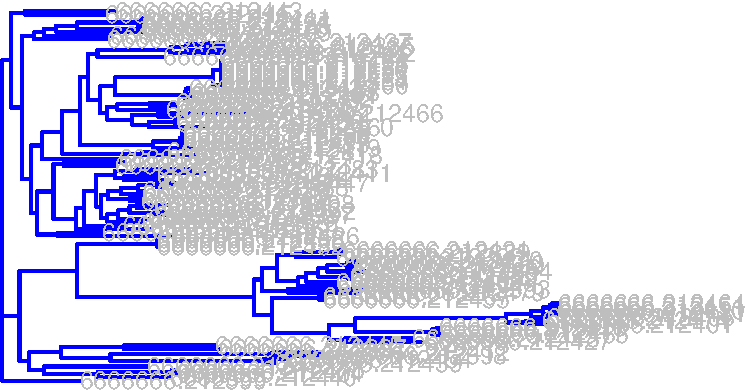
\includegraphics{tesis_files/figure-latex/testingPhylogeny-1} \end{center}
  
  To capture differences on genomes we sort them phylogenetically.
  Phylogenies can be constructed using different paradigms as Parsimony,
  Maximum Likelihood, and Bayesian inference. Short descriptions of the
  main phylogeny methods are included below.
  
  Why is a tree useful \{Book reference\} why trees are useful for?\\
  * Distance methods\\
  * Parsimony * Maximum Likelihood * Mr bayes
  
  General Trees\\
  Actinobacteria Tree, ArchaeaTree, CyanobacteriaTree.
  
  It's easy to create a list. It can be unordered like
  
  To create a sublist, just indent the values a bit (at least four spaces
  or a tab). (Here's one case where indentation is key!)
  
  \begin{enumerate}
  \def\labelenumi{\arabic{enumi}.}
  \tightlist
  \item
    Item 1
  \item
    Item 2
  \item
    Item 3
  
    \begin{itemize}
    \tightlist
    \item
      Item 3a
    \item
      Item 3b
    \end{itemize}
  \end{enumerate}
  
  \subsubsection{Central DB}\label{central-db}
  
  We chose central pathways from
  {[}\protect\hyperlink{ref-barona-gomez_what_2012}{9}{]}\\
  * BBH Best Bidirectional Hits with studied enzymes from Central
  Actinobacterial pathways were selected.
  
  \begin{itemize}
  \item
    By abundance
  \item
    By expansions on genomes
  \end{itemize}
  
  {[}largefiles,\url{https://help.github.com/articles/installing-git-large-file-storage/}{]}
  
  \section{Data Bases}\label{data-bases}
  
  \subsection{Central pathways}\label{central-pathways}
  
  Central database were chosen by BBH from
  
  \begin{Shaded}
  \begin{Highlighting}[]
  \NormalTok{table <-}\StringTok{ }\KeywordTok{read.csv}\NormalTok{(}\StringTok{"chapter1/WC_Central/BBH_Organisms.txt"}\NormalTok{, }\DataTypeTok{row.names =} \DecValTok{1}\NormalTok{,}\DataTypeTok{sep=}\StringTok{"}\CharTok{\textbackslash{}t}\StringTok{"}\NormalTok{)}
  \KeywordTok{kable}\NormalTok{(table,  }\DataTypeTok{caption =} \StringTok{"BBH_Organisms }\CharTok{\textbackslash{}\textbackslash{}}\StringTok{label\{tab:BBH_Organisms\}"}\NormalTok{,}\DataTypeTok{caption.short =} \StringTok{"BBH_Organisms "}\NormalTok{)}
  \end{Highlighting}
  \end{Shaded}
  
  \begin{longtable}[]{@{}lllll@{}}
  \caption{BBH\_Organisms \label{tab:BBH_Organisms}}\tabularnewline
  \toprule
  & RastId & Database & Taxa1 & Taxa2\tabularnewline
  \midrule
  \endfirsthead
  \toprule
  & RastId & Database & Taxa1 & Taxa2\tabularnewline
  \midrule
  \endhead
  Corynebacterium glutamicum & 6666666.112876 & Actinobacteria &
  &\tabularnewline
  Streptomyces coelicolor A3(2) NC\_003888.3 & & Actinobacteria &
  &\tabularnewline
  Mycobacterium tuberculosis H37Rv NC\_000962.3 & 6666666.146923 &
  Actinobacteria & &\tabularnewline
  Methanosarcina acetivorans C2A AE010299.1 & 6666666.211599 & Archaea &
  Euryarchaeota & Methanomicrobia\tabularnewline
  Nanoarchaeum equitans Kin4-M - AE017199.1 & 6666666.211718 & Archaea &
  DPANN group & Nanoarchaeota\tabularnewline
  Natronomonas pharaonis DSM 2160 & CR936257.1 & 6666666.211909 & Archaea
  & Euryarchaeota\tabularnewline
  Halobacteria & & & &\tabularnewline
  Sulfolobus solfataricus P2 AE006641.1 & 6666666.211567 & Archaea & TACK
  group & Crenarchaeota\tabularnewline
  Cyanothece sp. ATCC 51142 CP000806.1 & 6666666.212444 & Cyanobacteria &
  Oscillatoriales &\tabularnewline
  Synechococcus sp. PCC 7002 CP000951.1 & 6666666.212477 & Cyanobacteria &
  Synechococcales &\tabularnewline
  Arthrospira platensis C1 & 6666666.189647 & Cyanobacteria &
  Cyanobacteria &\tabularnewline
  \bottomrule
  \end{longtable}
  
  \subsection{Genome Dynamics}\label{genome-dynamics}
  
  Among BBH central databases, genomic dynamics was included.\\
  Whats change
  site:\href{http://pubseed.theseed.org/wc.cgi?request=show_otus\&base=/homes/nselem/Data/CS}{WC
  Data}
  
  groups were formed with 100Cyanos, 100Archaea , 118 Actinos Closed,
  43StreptosClosed\\
  Selected organims were
  
  \begin{Shaded}
  \begin{Highlighting}[]
  \NormalTok{table <-}\StringTok{ }\KeywordTok{read.csv}\NormalTok{(}\StringTok{"chapter1/WC_Central/WC_Organisms.txt"}\NormalTok{, }\DataTypeTok{row.names =} \DecValTok{1}\NormalTok{,}\DataTypeTok{sep=}\StringTok{"}\CharTok{\textbackslash{}t}\StringTok{"}\NormalTok{)}
  \KeywordTok{kable}\NormalTok{(table,  }\DataTypeTok{caption =} \StringTok{"WC_Organisms }\CharTok{\textbackslash{}\textbackslash{}}\StringTok{label\{tab:WC_Organisms\}"}\NormalTok{,}\DataTypeTok{caption.short =} \StringTok{"WC_Organisms "}\NormalTok{)}
  \end{Highlighting}
  \end{Shaded}
  
  \begin{longtable}[]{@{}lrl@{}}
  \caption{WC\_Organisms \label{tab:WC_Organisms}}\tabularnewline
  \toprule
  & Rast.Id & Database\tabularnewline
  \midrule
  \endfirsthead
  \toprule
  & Rast.Id & Database\tabularnewline
  \midrule
  \endhead
  Arthrospira platensis NIES-39 AP011615.1 & 6666666.21 &
  Cyanos\tabularnewline
  Synechococcus sp. PCC 7002 & 6666666.21 & Cyanos\tabularnewline
  Cyanothece sp. ATCC 51142 & 6666666.21 & Cyanos\tabularnewline
  Methanosarcina acetivorans & 6666666.21 & Archaea\tabularnewline
  Nanoarchaeum equitans Kin4-M & 6666666.21 & Archaea\tabularnewline
  Natronomonas pharaonis DSM 2160 & 6666666.21 & Archaea\tabularnewline
  Sulfolobus solfataricus P2 & 6666666.21 & Archaea\tabularnewline
  Mycobacterium tuberculosis H37Rv & 83332.23 & Actinos\tabularnewline
  Corynebacterium glutamicum ATCC 13032 & 196627.31 &
  Actinos\tabularnewline
  Streptomyces coelicolor A3(2) NC\_003888.3 & 6666666.11 & Actinos and
  Streptomyces\tabularnewline
  Streptomyces sp. Mg1 NZ\_CP011664.1 & 6666666.15 &
  Streptomyces\tabularnewline
  \bottomrule
  \end{longtable}
  
  Those families present on at least as much as genomes on the group\\
  Cyanos 100 647\\
  Abundant.Families.100Cyanos\\
  Actinos 118 132\\
  Abundant.Families.43Strepto\\
  Archaea 100 35\\
  Abundant.Families.Actinos\\
  Streptomyces 43 1263\\
  Abundant.Families.Archaeas
  
  Those families expanded on at least two groups\\
  \texttt{cat\ *Abun*\ \textbar{}\ cut\ -f3\textbar{}\ sort\ \textbar{}\ uniq\ -c\ \textbar{}\ sort\ \textgreater{}Abundance.all}\\
  
  Those Families expanded on Archaea and not expanded on Actino\\
  \texttt{comm\ -23\ f3Archaeas\ f3Actinos\ \textgreater{}ArchaeasNoActinos}\\
  Those Families expanded on Actino and not on Archaea\\
  \texttt{comm\ -13\ f3Archaeas\ f3Actinos\ \textgreater{}ActinosNoArchaea}
  
  Those families expanded on Streptomyces but not in ActinoBacteria\\
  \texttt{comm\ -13\ f343Strepto\ f3Actinos\ \textgreater{}ActinosNoStrepto}\\
  Those Families expanded on Actinobacteria and not in Streptomyces\\
  \texttt{comm\ -23\ f343Strepto\ f3Actinos\ \textgreater{}StreptoNoActinos}
  
  Those Families expanded on Cyano and not in Actino\\
  \texttt{comm\ -23\ f3Cyanos\ f3Actinos\ \textgreater{}CyanosNoActinos}
  
  \subsubsection{Natural Products DB}\label{natural-products-db}
  
  Natural products was improved from previous version
  
  \subsection{AntisMASH optional DB}\label{antismash-optional-db}
  
  AntiSMASH is {[}\protect\hyperlink{ref-weber_antismash_2015}{10}{]}\\
  \#\#\# Archaeas Results Archaea is a kingdom of recent discovery were
  not many natural products has been known. On Actinobacteria, evoMining
  has proved its value to find new kinds of natural products. The clue to
  this discovery was that Actinobacteria has genomic expanssions. Now
  Archaea has genomic expansions, even more has central pathways genomic
  expansions. Are this expansions derived from a genomic duplication?\\
  Has Archaea natural products detected by antismash, and if not, where
  are this NP's or may Archaea doesn't have NP's.
  
  applying EvoMining to Archaea
  
  \subsection{Otras estrategias para los clusters Argon context
  Idea}\label{otras-estrategias-para-los-clusters-argon-context-idea}
  
  \section{Argonne}\label{argonne}
  
  ssh
  \href{mailto:nselem@login.mcs.anl.gov}{\nolinkurl{nselem@login.mcs.anl.gov}}\\
  phrase\\
  ssh \href{mailto:nselem@maple}{\nolinkurl{nselem@maple}}\\
  password
  
  cs close strain\\
  wc whats chain
  
  we source (edit bashrc)\\
  link ln (create a link to ross directory)\\
  run out of power:\\
  screen
  
  in Seqs (not mine)\\
  cat\\
  6666666.103569 6666666.112815 6666666.112823 6666666.112833
  6666666.112841 6666666.112849 6666666.112857 \textgreater{}
  /home/nse/Concat\_Full\\
  to find paralogous sets\\
  svr\_representative\_sequences -b -f Id\_Clust -s 0.5 \textless{}
  Concat\_Full \textgreater{} TempFull\&\\
  perl -p -i -e `s/\r//' readable.tree to clean the tree\\
  To find contexts o pegs of paralogous sets
  
  Context midle point 5000 bp (using text tables)\\
  scp 6666666.112839.txt
  \href{mailto:nselem@maple}{\nolinkurl{nselem@maple}}:/homes/nselem/Strepto\_01/.
  
  fig\textbar{}6666666.112839.peg.26
  
  copy families.all file\\
  on the file we have column1 family name column 5 peg id
  
  cluster\_objects \textless{} elements\_to\_cluster \textgreater{}
  ClusteFile
  
  write a file with pegs\\
  1 peg1 adjacent1, adjacent2 \ldots{}.\\
  1 peg2\\
  2\\
  2
  
  write a file similiar but with the family number
  
  1 peg1 fn1, fn2 \ldots{}.\\
  1 peg2\\
  2\\
  2
  
  compare each peg on this file from the same family
  
  Write the conextions file\\
  peg1 peg2\\
  peg1 peg3\\
  peg2 peg3
  
  cluster this file and score the cluster
  
  Define
  
  \begin{verbatim}
  1.  a "function set" is generated by the what's changed directory  
  \end{verbatim}
  
  as a ``family''
  
  \begin{verbatim}
  2.  a "paralog set" is a set of function sets in which paralogous  
  \end{verbatim}
  
  members span the sets
  
  \begin{verbatim}
  3.  a PEG is in a paralog set if it is in one ofthe function sets  
  \end{verbatim}
  
  that make up the
  
  \begin{verbatim}
  4.  a "context" of a PEG is the set of close pegs  
  4.1 First cluster operation would give us: context sets  (CS)  
  
  5.  a "context set" is a set of PEGs with "similar contexts"  
  5.1 second clustering operation would give us:cluster  (Cl)  
  
  6.  a "cluster" is a set of context sets (each context set is a different   
  \end{verbatim}
  
  compute:\\
  Compute the context sets that are made from PEGs that occur in PS.\\
  Compute the contexts of PEGs in PS.
  
  cluster these context using the ``similar contexts'' relation
  
  This gives a set of clusters, and the members of the clusters are
  context sets\\
  That is, a cluster is a set of context sets
  
  \begin{verbatim}
    a. the number of contexts sets i  
  \end{verbatim}
  
  score the clusters\\
  Take a paralog set PS.\\
  Be the context sets: CS\_1, CS\_2,\ldots{}, CS\_k members of the
  paralogous set\\
  k the number of contexts sets on the paralogous set\\
  n\_i the cardinality of CS\_i
  
  \begin{verbatim}
  PS={CS1,CS2,...,CS3}  
  Cl={[CS_1,n_1],[CS_2,n_2],...,[CS_k,n_k]}  
  
  let be M=max(n_i)   i=1,2,..k (Maximum cardinality of Context sets)  
      m=max(n_i)   i=1,2,..k, i!=M (second greatest cardinality of context sets)  
      (We are intersted that a second copy is distributed)  
  
  We are interested on k,M,n to form a scoring function for the cluster set  
  S=f(k,m,M)=c_1*k+c_2*m+c_3*M  
  \end{verbatim}
  
  history
  
  Para hacer un nuevo set de datos
  
  591 cd Data/CS\\
  592 mkdir Directorio\\
  593 vi Directorio/rep.genomes\\
  594 cd Directorio/\\
  600 nohup svr\_CS -d Directorio\&
  
  Contenido de rep.genomes\\
  rast\textbar{}390693 nselem35 q8Vf6ib\\
  rast\textbar{}390675 nselem35 q8Vf6ib\\
  rast\textbar{}388811 nselem35 q8Vf6ib
  
  When you click the \textbf{Knit} button above a document will be
  generated that includes both content as well as the output of any
  embedded \textbf{R} code chunks within the document. You can embed an
  \textbf{R} code chunk like this (\texttt{cars} is a built-in \textbf{R}
  dataset):
  
  \begin{Shaded}
  \begin{Highlighting}[]
  \KeywordTok{summary}\NormalTok{(cars)}
  \end{Highlighting}
  \end{Shaded}
  
  \begin{verbatim}
       speed           dist       
   Min.   : 4.0   Min.   :  2.00  
   1st Qu.:12.0   1st Qu.: 26.00  
   Median :15.0   Median : 36.00  
   Mean   :15.4   Mean   : 42.98  
   3rd Qu.:19.0   3rd Qu.: 56.00  
   Max.   :25.0   Max.   :120.00  
  \end{verbatim}
  
  \subsection{Inline code}\label{inline-code}
  
  If you'd like to put the results of your analysis directly into your
  discussion, add inline code like this:
  
  \begin{quote}
  The \texttt{cos} of \(2 \pi\) is 1.
  \end{quote}
  
  Another example would be the direct calculation of the standard
  deviation:
  
  \begin{quote}
  The standard deviation of \texttt{speed} in \texttt{cars} is 5.2876444.
  \end{quote}
  
  One last neat feature is the use of the \texttt{ifelse} conditional
  statement which can be used to output text depending on the result of an
  \textbf{R} calculation:
  
  \begin{quote}
  The standard deviation is less than 6.
  \end{quote}
  
  Note the use of \texttt{\textgreater{}} here, which signifies a
  quotation environment that will be indented.
  
  As you see with \texttt{\$2\ \textbackslash{}pi\$} above, mathematics
  can be added by surrounding the mathematical text with dollar signs.
  More examples of this are in {[}Mathematics and Science{]} if you
  uncomment the code in {[}Math{]}.
  
  \section{Recomendaciones de Luis}\label{recomendaciones-de-luis}
  
  Para evoMining\\
  Probar distintos métodos de filogenia y después hacer la coloración.\\
  maximum likelihood, Protest phyml\\
  Atracción de ramas largas.\\
  raxml\\
  trim all vs Gblocs (Tony Galvadon)
  
  Comparar dos árboles\\
  Para ver si la evolución de los genes concatenados ha sido simultánea\\
  Robinson and foulds\\
  Joe Felsestein\\
  Phylip
  
  \begin{enumerate}
  \def\labelenumi{\arabic{enumi}.}
  \setcounter{enumi}{1}
  \tightlist
  \item
    dist tree\\
    quarter descomposition\\
    peter gogarten fendou Mao
  \end{enumerate}
  
  Sets de experimentos.\\
  Para el experimento de los streptomyces con ruta centrales el core,
  analizar el problema de dominios múltiples.\\
  Dominios\\
  Nan Song, Dannie durand\\
  Después del blast
  
  Para obtener\\
  Pablo Vinuesa: Get Homologues
  
  Burkhordelias y su toxina (Preguntar a Beto)\\
  Cianobacterias y la ruta de fijación de nitrógeno.
  
  Servidor Viernes a las 12:00
  
  \section{CORASON: Other genome Mining tools
  context-based}\label{corason-other-genome-mining-tools-context-based}
  
  \section{CORe Analysis of Syntenic Orthologs to prioritize Natural
  Product-Biosynthetic Gene
  Cluster}\label{core-analysis-of-syntenic-orthologs-to-prioritize-natural-product-biosynthetic-gene-cluster}
  
  Bacterial biosynthetic gene clusters (BGCs) known are always increasing,
  almost all bacterial genome sequenced contributes with new genes and
  gene clusters to the known Bacterial Pangenome. In consequence of gene
  diversity and sequence technology advances researchers often have a
  large set of genomes to analize in search of a particular gene cluster
  variation. Answering BGCs analysis needs, CORASON allows users to find
  and visualice variations of a given gene cluster sorting them according
  to the conserved core cluster phylogeny.
  
  The core genome on a taxonomical group is the set of coding sequences
  that are shared between all group members, this definition may be
  adapted to the cluster core by exploring a set of gene clusters instead
  of a set of genomes. The cluster core attempts to identify a set of
  functions conserved on a particular BGC variations. A report about gene
  function using RAST technology will be provided whenever a cluster core
  exists and core sequences will be concatenated to construct a
  phylogenetic tree and sort variation clusters accordingly.
  
  To find cluster variations, given a query protein sequence that belongs
  to a reference cluster, CORASON will search on a Bacterial genome
  database all gene clusters that contains orthologues of the
  query-protein and at least another sequence from the reference cluster.
  Orthologues on variation clusters are coloured within a gradient
  according to its identity percentage with the reference cluster
  sequences.
  
  Finally, in order to provide an easy to install distribution, CORASON
  was packaged on docker containerization platform. Software dependencies
  such as BLAST 2.2.30, muscle3.8.3, GBlocksLinux64\_0.91b, quicktree,
  newick-utils-1.6, and CORASON code were wrapped together on CORASON
  docker container.
  \href{https://github.com/nselem/EvoDivMet/wiki}{Tutorial} and software
  are available at nselem/github.
  
  CORASON inputs are a genomic database, a reference cluster and an enzyme
  inside this cluster, outputs are newick trees, core functional report
  and a cluster variation SVG file. SVG format among being high quality
  scalable graphics, also allow to display metadata such as gene function
  and genome coordinates just by mouse over figures on a browser
  facilitating genomic analysis.
  
  In conclusion CORASON is an easy to install comparative genomic visual
  tool on a customizable genome database that allows users to visualice
  variations of a reference gene cluster identifing its core functions and
  finally sorting variations according to their evolutionary history
  helping to prioritize clusters that may be involved on chemical novelty.
  
  \section{Tree methods (from antiSMASH textual
  quotation)}\label{tree-methods-from-antismash-textual-quotation}
  
  \emph{Multiple methods exist to construct phylogenetic trees based on
  multiple sequence alignments. Depending on the desired output tree
  characteristics, the number of input sequences, and other constraints,
  the most appropriate method should be chosen. A popular algorithm among
  the distance-matrix based methods is the Neighbour-Joining algorithm
  that uses bottom-up clustering to create the tree. Neighbour-Joining is
  comparatively fast method, but the correctness of the tree depends on
  the accuracy and additivity of the underlying distance matrix. Maximum
  parsimony methods try to identify the tree that uses the smallest number
  of evolution events to explain the observed sequence data. While maximum
  parsimony algorithms build very accurate trees, their computation tends
  to be relatively slow compared to distance-matrix based methods. Maximum
  likelihood methods use probability distributions to assess the
  likelihood of a given 5
  \url{http://mc.manuscriptcentral.com/bibManuscripts} submitted to
  Briefings in Bioinformatics phylogenetic tree according to a
  substitution model. This method unfortunately has a high complexity for
  computing the optimal tree. Many current tools use a combination of
  methods}
  
  \chapter*{Background}\label{background}
  \addcontentsline{toc}{chapter}{Background}
  
  Enzymes catalice chemical reactions transforming substrates into
  producs. During 20th century enzymes were percived as highly specific
  catalizer, nevertheless this percepcion changed with the discovery that
  they can . This abilty to catalice several chemical functions its known
  as enzyme promscuity. Escherichia coli contains at least 404 promiscuous
  enzymes. La relevancia de la promiscuidad radica tanto en su papel como
  mecanismo de evolucion de la funcion enzimatica, asi como en la
  necesidad de su deteccion para la correccion de modelos de flujo
  metabolico y la determinacion de efectos secundarios en drogas
  farmacologicas. A pesar de su frecuencia e importancia aun se esta en el
  proceso de entender las causas y las caracteristicas observables de la
  promiscuidad enzimatica.
  
  Para estudiar la promiscuidad esta propuesta discierne entre dos
  problemas. El primero es el de ubicar cuales familias tienen enzimas
  promiscuas, al que llamaremos problema de las familias. El segundo es el
  de los miembros: una vez identificada una familia promiscua, como
  distinguir entre sus miembros enzimas con distinto nivel de
  promiscuidad. Se ha intentado identificar enzimas promiscuas, a nivel de
  secuencia, sin pasar por experimentacion mediante aprendizaje maquina.
  Estos enfoques son incapaces de identificar una familia promiscua si no
  se conoce previamente al menos un miembro promiscuo de ella. Por otra
  parte, en el problema de los miembros se presentan dificultades cuando
  la identidad de secuencia es alta, e.g.~en la familia PriA-HisA se sabe
  que la enzima HisA de E. coli no es promiscua, pero PriA de Streptomyces
  coelicolor si lo es.
  
  Para mejorar nuestro entendimiento del fenomeno, ademas de la
  comparacion de secuencias es necesario integrar otros elementos de
  analisis. Se debe notar que es practicamente imposible decir que una
  enzima no es promiscua ya que para ello se deberian haber descartado
  todos los posibles sustratos. Sin embargo, para el estudio de cambios en
  promiscuidad se han detectado como elementos relevantes a los cambios en
  vecindad genomica, los cambios en flexibilidad durante la dinamica
  molecular, la perdida de genes centrales, y finalmente a las expansiones
  genicas dentro de un grupo taxonomico. Estos elementos tienen en comun
  que reflejan un cambio en alguna propiedad genomica o biofisica, de lo
  que se deriva que el buscar cambios en la promiscuidad de una enzima
  resulta mas factible que la busqueda intrinseca de promiscuidad, a lo
  que aspiran los metodos basados en comparaciones de secuencias.
  
  Evomining es una plataforma bioinformatica pensada para la busqueda de
  expansiones de familias genicas de metabolismo central. Desarrollarla en
  combinacion con algoritmos de busqueda de cambios en la vecindad
  genomica la haran una plataforma ideal para abordar el problema de las
  familias, proporcionando una solucion a la dificultad de no tener
  conocimiento previo de un miembro promiscuo en la familia investigada.
  Respecto al problema de los miembros, se propone explorar variaciones en
  vecindad genomica, flujo genico y dinamica molecular, como candidatos a
  reflejar la variacion en promiscuidad. Finalmente, he detectado que a
  pesar de que pruebas in vivo son mas sensibles a niveles bajos de
  promiscuidad que mediciones in vitro, esta ultima suele ser la unica
  estudiada. In vivo, la metabolomica aplicada en genes biosinteticos de
  productos naturales ha ayudado en la identificacion de sustratos, por lo
  que esta tecnica podria ayudar a revelar el nuevo sustrato de una enzima
  en la que se sospecha ganancia de promiscuidad. En resumen, el objetivo
  de mi trabajo sera abordar los dos problemas de promiscuidad
  considerando la diferenciacion in vitro e in vivo tomando como modelo
  biologico el phylum Actinobacteria, un grupo de bacterias reconocido por
  su diversidad metabolica donde se ha probado la existencia de
  promiscuidad enzimatica.
  
  \section{Introduction}\label{introduction-1}
  
  Para estudiar la promiscuidad es necesario contar con una definicion,
  algunos autores emplean el termino promiscuidad para describir
  actividades enzimaticas distintas a la funcion principal
  {[}\protect\hyperlink{ref-khersonsky_enzyme_2010}{12}{]} otros lo ven
  como una actividad secundaria fortuita
  {[}\protect\hyperlink{ref-copley_enzymes_2003}{13}{]} que pudo aparecer
  de forma accidental o inducida artificialmente
  {[}\protect\hyperlink{ref-hult_enzyme_2007}{14}{]}. Otros mas, cuando
  una enzima puede operar sobre un amplio rango de sustratos, prefieren
  llamarla multiespecifica
  {[}\protect\hyperlink{ref-khersonsky_enzyme_2010}{12}{]}. A la accion de
  realizar distintas funciones cataliticas, ya sea al catalizar varias
  reacciones quimicas o bien una misma reaccion en sustratos diferentes se
  le conoce como promiscuidad enzimatica
  {[}\protect\hyperlink{ref-obrien_catalytic_1999}{15}{]}. Existen varios
  tipos de promiscuidad enzimatica.
  
  Por sustrato cuando la reaccion es la misma pero se lleva a cabo en
  distintos sustratos ejemplo la familia PriA
  {[}\protect\hyperlink{ref-baronagomez_occurrence_2003}{16}{]} y la
  familia de betalactamasas
  {[}\protect\hyperlink{ref-risso_phenotypic_2014}{17}{]}
  
  Catalitica cuando la enzima utiliza diferentes mecanismos de reaccion
  y/o residuos cataliticos, e.g.~la quimotripsina puede catalizar
  reacciones de amidasa y fosfotriesterasa en un mismo sitio activo.
  {[}\protect\hyperlink{ref-obrien_catalytic_1999}{15}{]} Por condiciones
  del entorno, cuando la enzima cambia su conformacion dependiendo de las
  condiciones quimicas y fisicas presentes como pH, temperatura, solventes
  organicos y salinidad e.g.~algunas lipasas pueden actuar como
  sintetizadoras de esteres en lugar de hidrolasas en presencia de
  solventes organicos {[}\protect\hyperlink{ref-hult_enzyme_2007}{14}{]}.
  
  Este trabajo se enfocara a la promiscuidad por sustrato, entendiendo asi
  que la enzima es capaz de catalizar la misma reaccion quimica en al
  menos dos sustratos. La promiscuidad por sustrato es importante en
  terminos evolutivos, por ejemplo la enzyme commission number (EC) separa
  las enzimas en clases, a cada enzima se asignan 4 digitos, los tres
  primeros corresponden a la reaccion y el ultimo al sustrato; el mayor
  numero de sustratos (4306 clases) que de reacciones quimicas (234 en el
  tercer nivel) sugiere que la mayor variacion evolutiva se da a nivel de
  sustrato y no de reaccion
  {[}\protect\hyperlink{ref-li_computational_2004}{19}{]}. Otra evidencia
  de la importancia de la multiespecificidad por sustrato esta en el
  descubrimiento de las superfamilias, enzimas mecanistica y
  estructuralmente relacionadas que divergen en su afinidad por sustrato
  {[}\protect\hyperlink{ref-glasner_evolution_2006}{20}{]}
  
  Si bien existen familias de enzimas con alta especificidad por sustrato,
  otras familias como el citocromo P450
  {[}\protect\hyperlink{ref-bloom_neutral_2007}{22}{]} y las beta
  lactamasas {[}\protect\hyperlink{ref-zou_evolution_2015}{24}{]} son
  promiscuas. Es posible que la vision previa de alta especificidad se
  deba a que las primeras rutas metabolicas estudiadas pertenecen al
  metabolismo central, donde la especificidad puede haber sido favorecida
  por presiones de seleccion
  {[}\protect\hyperlink{ref-firn_darwinian_2009}{25}{]}. Esta vision ha
  cambiado debido al conocimiento de mas enzimas con multifuncionalidad
  {[}\protect\hyperlink{ref-jia_multifunctional_2013}{26}{]}, sin afectar
  la eficiencia catalitica por la funcion primaria
  {[}\protect\hyperlink{ref-aharoni_evolvability_2005}{27}{]}. En 1976 el
  interes por la promiscuidad comenzo por su influencia en la evolucion de
  la funcion
  enzimatica{[}\protect\hyperlink{ref-jensen_enzyme_1976}{28}{]}, las
  aproximaciones variaron desde la aparicion de la sintesis funcional
  {[}\protect\hyperlink{ref-dean_mechanistic_2007}{30}{]}, cuando la
  disponibilidad de genomas permitio la combinacion de analisis
  filogeneticos con tecnicas de biologia molecular, bioquimica y biofisica
  (Fig 1). En 2003 la biofisica de las proteinas entra en escena al
  postularse que la diversidad conformacional durante la dinamica
  molecular debe incidir en la aceptacion de distintos sustratos.
  Recientemente se ha investigado su papel en efectos secundarios en
  drogas farmacologicas
  {[}\protect\hyperlink{ref-nobeli_protein_2009}{31}{]}. Entre 2005 y 2010
  se avanza del estudio de una sola familia enzimatica hacia el interes
  por propiedades globales, por ejemplo dado un genoma se investiga la
  distribucion de familias promiscuas en subsistemas metabolicos. En estos
  años, surge el desarrollo de indices que reflejen las caracteristicas
  bioquimicas de enzimas promiscuas. En 2010, comienzan los intentos por
  desarrollar un metodo computacional de prediccion de promiscuidad. Desde
  2012 a la fecha, a la par que las aproximaciones bioinformaticas se
  multiplican, se desarrollan investigaciones de aspectos biofisicos,
  bioquimicos y evolutivos de enzimas promiscuas reafirmando que todos
  estos aspectos estan relacionados al fenomeno. En las siguientes
  secciones se describiran trabajos importantes sobre la relacion que
  guarda la promiscuidad con expansiones genomicas y flexibilidad
  molecular. Ademas se hablara sobre analisis bioquimicos y metabolicos
  para la descripcion del fenomeno.
  
  \TeX~or \LaTeX~\\
  \#\#\# Funcion biologica de la promiscuidad enzimatica\\
  ¿Por que existe la promiscuidad enzimatica? Se tiene evidencia de dos
  papeles biologicos: el primero proporcionar robustez a la red metabolica
  de un organismo mediante redundancia de reacciones de otras enzimas; el
  segundo permitir plasticidad evolutiva, es decir materia prima para la
  adaptacion a variaciones ambientales
  {[}\protect\hyperlink{ref-aharoni_evolvability_2005}{27}{]} mediante la
  adquisicion de nuevas funciones quimicas. Respecto a la robustez, se
  probo que sobreexpresar enzimas promiscuas puede rescatar perdidas
  genicas {[}\protect\hyperlink{ref-patrick_multicopy_2007}{38}{]}. De 104
  knockout sencillos de genes esenciales para E. coli K-12, 20\% de las
  auxotrofias pudieron ser suprimidas por la sobreexpresion de plasmidos
  que contenian enzimas promiscuas. Otro ejemplo que aporta a la robustez
  es PriA, enzima de la ruta de histidina que realiza en la ruta del
  triptofano la reaccion E.C. 5.3.1.24
  {[}\protect\hyperlink{ref-baronagomez_occurrence_2003}{16}{]}. En cuanto
  a la plasticidad se propone que para que la promiscuidad pueda dar
  origen a la aparicion de nuevas funciones la actividad promiscua debe
  proveer una ventaja fisiologica inmediata para poder ser seleccionada
  positivamente, ademas una vez que una funcion promiscua se vuelva
  relevante se debe poder mejorar mediante pocas mutaciones derivando en
  el intercambio entre la actividad promiscua y la
  principal{[}\protect\hyperlink{ref-khersonsky_enzyme_2010}{12}{]}.
  
  Aun cuando el producto de la promiscuidad genera metabolitos que no se
  integran al metabolismo central de la celula, su efecto es positivo ya
  que estos metabolitos podrian colaborar a la adaptacion al entorno
  participando por ejemplo en una relacion de simbiosis o de competencia
  con otros organismos. Este tipo de metabolitos, por lo general, no son
  dañinos {[}\protect\hyperlink{ref-notebaart_network-level_2014}{39}{]} y
  pueden servir como bloques de construccion para vias metabolicas nuevas
  {[}\protect\hyperlink{ref-ma_unconventional_2013}{42}{]}. La respuesta
  inmediata de adaptacion de un organismo podria ser una consecuencia de
  su grado de promiscuidad.
  
  \subsection{Relacion del pangenoma con la promiscuidad
  enzimatica}\label{relacion-del-pangenoma-con-la-promiscuidad-enzimatica}
  
  El core genome de un grupo taxonomico es el conjunto de secuencias
  codificantes presentes en todos los organismos del grupo. En el Dominio
  Bacteria el core esta estimado entre 200 y 300 secuencias
  {[}\protect\hyperlink{ref-halachev_calculating_2011}{3}{]}. Dada su
  conservacion el core genome puede utilizarse para trazar mejores
  relaciones filogeneticas que las obtenidas con el uso exclusivo de
  marcadores como la subunidad 16s del RNA ribosomal o el gen rpoB. El
  pangenoma es el conjunto complemento del core genome, es decir todas
  aquellas secuencias que estan ausentes de uno o mas organismos del grupo
  y por lo tanto no son necesarias para todos, sino solo posiblemente para
  el organismo que las posee. Como en el pangenoma la presion de seleccion
  esta relajada respecto al core-genome
  {[}\protect\hyperlink{ref-firn_darwinian_2009}{25}{]} es el conjunto
  donde la plasticidad genomica tiene facilidades para desarrollarse.
  
  Esta idea puede restringirse a subsistemas metabolicos para identificar
  genes cuyas enzimas estan en proceso de cambio de funcion quimica, por
  ejemplo, en este trabajo se encontro que el gen trpF esta presente en
  solo 49 de 290 genomas analizados del genero Streptomyces por lo que se
  encuentra en el pangenoma de triptofano de este genero taxonomico,
  posiblemente adquiriendo una nueva funcion
  {[}\protect\hyperlink{ref-ma_unconventional_2013}{42}{]}. Para evitar
  problemas tecnicos del calculo del pangenoma existen otros modelos de
  medicion de variabilidad del genomica entre especies bacterianas
  {[}\protect\hyperlink{ref-kislyuk_genomic_2011}{45}{]}.
  
  \subsection{Expansion y contextos genomicos como herramienta de
  anotacion
  funcional}\label{expansion-y-contextos-genomicos-como-herramienta-de-anotacion-funcional}
  
  La diversidad enzimatica existente es el resultado de un proceso de
  expansion, mutacion y seleccion que se ha desarrollado durante el
  transcurso de la historia evolutiva
  {[}\protect\hyperlink{ref-khersonsky_enzyme_2010}{12}{]}. Existe
  evidencia de que cierto grado de promiscuidad o divergencia funcional
  precede a la duplicacion genica
  {[}\protect\hyperlink{ref-hughes_evolution_1994}{47}{]}. Por este motivo
  detectar expansiones ya sea duplicaciones o transferencias horizontales
  {[}\protect\hyperlink{ref-treangen_horizontal_2011}{48}{]}, puede ser un
  buen punto de partida para determinar divergencia funcional y
  promiscuidad. No todas las expansiones denotan cambio de funcion
  enzimatica, algunas pueden ser meros accidentes, sin embargo dado que la
  funcion de una enzima suele estar relacionada con sus vecinos
  {[}\protect\hyperlink{ref-overbeek_use_1999}{49}{]}, una expansion en
  una vecindad genomica diferente de la tradicional sera un referente de
  adquisicion de una nueva funcion y entonces un indicador de existencia
  previa de promiscuidad.
  
  La funcion de una enzima es un concepto jerarquico, dependiente de la
  filogenia de un organismo
  {[}\protect\hyperlink{ref-szklarczyk_string_2015}{53}{]}. Para
  sistematizar el estudio de contextos y vecindades genomicas se
  desarrollo Search Tool for the Retrieval of Interacting Genes/Proteins
  STRING {[}\protect\hyperlink{ref-snel_string:_2000}{54}{]}, que cuenta
  con una anotacion de ortologia jerarquica y consistente, realizada en
  2000 organismos en cuyo marco interacciones de proteinas con
  implicaciones funcionales son predichas tanto de novo por informacion
  genomica de co-ocurrencia como por mineria de datos en articulos
  publicados. STRING es una base de datos, y como tal no permite agregar
  nuevos genomas para su analisis. Sus 2000 organismos incluyen especies
  tanto bacterianas como eucariotas. Al existir tanta diversidad, los
  genomas disponibles para un genero o clase especificos son escasos,
  p.~g. de los mas de 300 genomas disponibles de Streptomyces solo 24
  estan incluidos.
  
  Para resolver la baja cobertura de STRING hacia ciertos grupos
  taxonomicos se pueden desarrollar scripts de vecindad genomica
  utilizando RAST (Rapid Annotation using Subsystem Technology); un
  servicio interactivo de anotacion automatica de genomas de bacterias y
  arqueas {[}\protect\hyperlink{ref-aziz_rast_2008}{5}{]} donde la funcion
  de cada gen se asigna de acuerdo a conocimiento previo de subsecuencias
  de organismos cercanos filogeneticamente, cuando es posible se incluye
  en un subsistema metabolico. Estamos en una era de explosion de datos
  genomicos, proximamente se espera contar con millones de genomas
  bacterianos incluso provenientes de bacterias no cultivables, por ello
  los algoritmos deben ser constantemente optimizados a los nuevos
  volumenes de datos
  {[}\protect\hyperlink{ref-medema_computational_2015}{55}{]}. Ante esta
  expectativa seria muy util desarrollar algoritmos de analisis genomico
  que sean de codigo libre o al menos interactivos para que cada
  laboratorio pueda personalizarlos para sus propios genomas.
  
  Finalmente, no solo la vecindad genomica inmediata puede ser utilizada
  como distintivo en la busqueda de promiscuidad, diferencias en el
  contexto genomico en genes relacionados con una enzima promiscua, sin
  importar su ubicacion dentro del genoma tambien pueden ser relevantes
  para la perdida o ganancia de funcion quimica
  {[}\protect\hyperlink{ref-noda-garcia_evolution_2013}{56}{]}, (Juarez
  Vazquez et al 2015).
  
  \subsection{Modelos bioinformaticos de
  promiscuidad}\label{modelos-bioinformaticos-de-promiscuidad}
  
  Con el fin de reducir la inversion en el proceso de experimentacion, se
  han implementado en los ultimos años algoritmos computacionales para
  predecir promiscuidad enzimatica
  {[}\protect\hyperlink{ref-carbonell_molecular_2010}{57}{]}. Estos
  procedimientos cuentan con un conjunto de aprendizaje, unos descriptores
  del conjunto, una fase de ajuste de parametros y finalmente una
  prediccion. En 2010, Carbonell propone un algoritmo de soporte vectorial
  basado en subsecuencias de distinto tamaño que llama huellas
  moleculares. En este trabajo aplicado sobre 500,000 proteinas reportadas
  en la enciclopedia de Kyoto de genes y genomas (KEGG) se reporta 85\% de
  exito en deteccion de enzimas promiscuas anotadas en KEGG. En 2012,
  Cheng compara los metodos de random forest y soporte vectorial en 6799
  proteinas provenientes de la base de datos Universal Protein Resource
  (UniProt). Las enzimas son descritas con subsecuencias de aminoacidos
  incorporando ademas caracteristicas biofisicas como polaridad. Se
  utiliza como grupo de control a familias de enzimas donde nunca se ha
  reportado una enzima promiscua.
  
  Un aspecto no considerado en estos metodos es que hay familias de
  enzimas con alta identidad de secuencia entre sus miembros, con cambios
  bruscos en promiscuidad, debidos por ejemplo a la dinamica genomica
  {[}\protect\hyperlink{ref-noda-garcia_evolution_2013}{56}{]}, lo que
  dificulta que considerar solo la secuencia conlleve a buenos predictores
  de promiscuidad. Cuando se obtiene una prediccion positiva utilizando
  los modelos existentes, lo que significa es que dada esa secuencia, en
  su familia se conoce previamente un elemento promiscuo y que ademas sus
  subsecuencias de cierto tamaño son suficientemente similares. Estos
  enfoques no pueden predecir de novo, en familias donde la promiscuidad
  no ha sido previamente detectada experimentalmente, pues no consideran
  aspectos evolutivos ni mecanisticos de las enzimas.
  
  Otra limitante a los enfoques descritos es que mezclan en su conjunto de
  entrenamiento fenomenos distintos de promiscuidad. Cheng p.~g. incluye
  enzimas moonlight que si bien poseen funciones adicionales a la
  catalizacion, son distantes a las enzimas promiscuas
  {[}\protect\hyperlink{ref-copley_enzymes_2003}{13}{]}. Ademas en ambos
  casos mezclan en el mismo conjunto enzimas bacterianas y eucariotas, con
  lo que si existia una huella basada en secuencia entonces esta puede
  diluirse por la gran distancia taxonomica entre estos grupos (Tabla 1).
  
  \subsection{Promiscuidad in vitro y promiscuidad in
  vivo}\label{promiscuidad-in-vitro-y-promiscuidad-in-vivo}
  
  La ganancia de promiscuidad no solo puede entenderse como la capacidad
  de convertir mas sustratos
  {[}\protect\hyperlink{ref-carbonell_molecular_2010}{57}{]}, sino tambien
  como la mejora de la capacidad catalitica respecto a ellos. El I-index
  {[}\protect\hyperlink{ref-nath_quantitative_2008}{23}{]}, esta definido
  como un rango de valores entre 0 y 1 que tiende a 1 entre mas parecida
  sea la actividad de la enzima sobre distintos sustratos, la capacidad
  catalitica es medida en terminos del cociente de Michaelis - Menten
  \(\frac{K_{cat}}{K_m}\). El indice ha sido utilizado para predecir la
  afinidad por sustrato del citocromo P450
  {[}\protect\hyperlink{ref-nath_quantifying_2010}{33}{]}. Una limitante
  del indice \(I\) es que se deben conocer los sustratos a los que la
  enzima es afin; sin embargo se puede sospechar que una enzima ha ganado
  promiscuidad aun sin conocer sus potenciales sustratos. Otro punto a
  señalar es que las variables Kcat,Kmson mediciones realizadas in vitro y
  no se consideran todos los sustratos presentes in vivo. Para solventar
  esta dificultad e investigar variaciones de sustratos nativos se pueden
  buscar productos similares a los ya conocidos por medio de analisis
  metabolicos {[}\protect\hyperlink{ref-nesvizhskii_analysis_2007}{62}{]}
  como los empleados en la deteccion de rutas no conservadas en la
  biosintesis de productos naturales
  {[}\protect\hyperlink{ref-medema_computational_2015}{55}{]}. En
  particular para este fin se ha utilizado espectrometria de masas MS/MS,
  {[}\protect\hyperlink{ref-nesvizhskii_analysis_2007}{62}{]} combinada
  con molecular networking para identificar productos similares
  {[}\protect\hyperlink{ref-yang_molecular_2013}{64}{]}
  
  \subsection{El papel de la dinamica molecular en la
  promiscuidad}\label{el-papel-de-la-dinamica-molecular-en-la-promiscuidad}
  
  La estructura tridimensional de una proteina es obtenida mediante previa
  purificacion y cristalizacion. Aunque mucho se ha hablado de la relacion
  estructura funcion, al cristalizar se obtienen estados conformacionales
  homogeneos, que bien pueden no ser la unica conformacion que adopta la
  proteina en solucion.
  {[}\protect\hyperlink{ref-james_conformational_2003}{66}{]}. En
  particular en el problema de promiscuidad, se ha observado que la
  variacion funcional no queda obviamente reflejada en la variacion
  estructural, lo que sugiere un rol significativo para la dinamica
  molecular {[}\protect\hyperlink{ref-parisi_conformational_2015}{67}{]}.
  Se postula que un aspecto de la dinamica molecular relevante para la
  diversificacion de especificidad por sustrato es el numero de
  conformeros {[}\protect\hyperlink{ref-javier_zea_protein_2013}{68}{]}.
  Por ejemplo, en la actinobacteria Corynebacterium diphtheriae parece que
  el contexto genomico correlaciona con perdida de promiscuidad de PriA ya
  que al poseer el genoma una copia de trpF, la enzima perdio esta funcion
  quimica conservando solo la funcion EC 5.3.1.16 correspondiente a la
  ruta de histidina. Esta sub-funcionalizacion se refleja en la perdida de
  estados conformacionales cambiando desde 1 estado en C. diphtheriae
  hasta 4 presentes en la dinamica de PriA de M. tuberculosis
  {[}\protect\hyperlink{ref-noda-garcia_evolution_2013}{56}{]}.
  
  Las regiones rigidas de una enzima proporcionan orientacion adecuada con
  respecto a los grupos cataliticos, mientras que las regiones flexibles
  permiten al sitio activo adaptarse a los sustratos con diferentes formas
  y tamaños {[}\protect\hyperlink{ref-copley_enzymes_2003}{13}{]}. Esta
  consideracion sugiere que la flexibilidad del sitio activo es otra
  caracteristica de la dinamica molecular a considerar para obtener
  informacion de la capacidad de ligacion de una enzima a distintos
  sustratos
  {[}\protect\hyperlink{ref-gatti-lafranconi_flexibility_2013}{69}{]}.
  Recientemente el indice de flexibilidad dinamica (dfi) se utilizo como
  una medida cuantitativa basado en la respuesta a perturbaciones de
  aminoacidos (PRS). Este indice se incremento en regiones cercanas al
  sitio activo de beta lactamasas promiscuas respecto al correspondiente
  dfi de \(\noindent\beta\) -lactamasas especialistas existentes
  {[}\protect\hyperlink{ref-zou_evolution_2015}{24}{]}.
  
  \subsection{Modelo biologico diversidad de
  Actinobacteria}\label{modelo-biologico-diversidad-de-actinobacteria}
  
  Al escoger un conjunto acotado para investigar familias de enzimas
  promiscuas se debe recordar que la funcionalidad es jerarquica por lo
  que para mejorar la anotacion, es deseable reflejar el proceso evolutivo
  y restringirse a un grupo de organismos taxonomicamente relacionados
  {[}\protect\hyperlink{ref-cruz-morales_phylogenomic_2016}{1}{]}.
  Actinobacteria es un phylum que posee promiscuidad tanto en el
  metabolismo periferico como en el core metabolico. Entre datos publicos
  (NCBI) y privados estan disponibles alrededor de 1200 genomas no
  redundantes de especies de Actinobacteria. Como punto de partida, se han
  estudiado las relaciones filogeneticas y grupos de ortologia
  {[}\protect\hyperlink{ref-li_orthomcl_2003}{70}{]}, en particular en
  Actinobacteria para identificar relaciones entre las familias del
  phylum, se obtuvieron arboles multilocus de entre 100 y 157 genomas
  {[}\protect\hyperlink{ref-gao_phylogenetic_2012}{72}{]}. Estos estudios
  sugieren como separar los genomas disponibles para hacer el calculo de
  grupos de ortologia. Finalmente, se han realizado estudios de
  plasticidad genomica en Streptomyces considerando 5 y 17 organismos de
  los 300 genomas disponibles en la actualidad
  {[}\protect\hyperlink{ref-zhou_genome_2012}{74}{]} donde reportan 2,018
  familias en el core genome y 32,574 en el pangenoma.
  
  \subsection{Modelo metabolico biosintesis de
  aminoacidos.}\label{modelo-metabolico-biosintesis-de-aminoacidos.}
  
  Al hacer el calculo vemos que Streptomyces, un genero del phylum
  Actinobacteria cuenta en su genoma con un promedio de 8316 secuencias
  codificantes segun la especie. Gran parte de estas secuencias pueden ser
  agrupadas en subsistemas metabolicos como metabolismo de carbohidratos o
  de lipidos; de estos subsistemas uno de los mas amplios es el
  metabolismo de aminoacidos con entre 429 y 910 secuencias segun el
  organismo. La sintesis de aminoacidos es un subsistema presente en todas
  las especies pero con suficientes variaciones que permiten hacer
  observaciones evolutivas. En un gran numero de Actinobacterias las rutas
  de histidina y triptofano de 7 y 11 pasos respectivamente convergen en
  una enzima bifuncional llamada PriA, que realiza tanto la funcion de
  HisA como la de TrpF
  {[}\protect\hyperlink{ref-baronagomez_occurrence_2003}{16}{]}. La
  cantidad de familias en el subsistema de metabolismo de aminoacidos, su
  variabilidad, su conservacion entre distintos grupos taxonomicos y la
  existencia de estos ejemplos en Actinobacteria lo posicionan como un
  buen punto de partida para la busqueda de promiscuidad tanto de familias
  promiscuas como de miembros promiscuos de las mismas.
  
  \section{Antecedentes}\label{antecedentes}
  
  En las cuatro decadas de estudio de la promiscuidad enzimatica, hemos
  aprendido que es un fenomeno distribuido en distintos subsistemas
  metabolicos {[}\protect\hyperlink{ref-nam_network_2012}{76}{]} y que su
  existencia puede deberse tanto al desarrollo de nuevas funciones para
  fines adaptativos {[}\protect\hyperlink{ref-jensen_enzyme_1976}{28}{]},
  como al rescate de una funcion perdida
  {[}\protect\hyperlink{ref-patrick_multicopy_2007}{38}{]}. Por ello la
  dinamica de perdida y ganancia de genes asociada al contexto genomico en
  bacterias se relaciona con cambio en la funcion enzimatica
  {[}\protect\hyperlink{ref-zhao_discovery_2013}{51}{]}. Precisando,
  respecto a la ganancia de genes, se postula que la bifuncionalidad
  precede la duplicacion
  {[}\protect\hyperlink{ref-hughes_evolution_1994}{47}{]}. Lo que implica
  que dada una duplicacion muy posiblemente previamente la promiscuidad
  estuvo presente {[}\protect\hyperlink{ref-gerlt_divergent_2001}{78}{]}.
  
  Se han desarrollado tecnicas bioquimicas y metabolicas de medicion
  {[}\protect\hyperlink{ref-nath_quantitative_2008}{23}{]}, asi como
  algoritmos computacionales de prediccion de promiscuidad
  {[}\protect\hyperlink{ref-carbonell_molecular_2010}{57}{]}. Un aspecto a
  mejorar dentro del modelado es la restriccion del conjunto de estudio a
  un grupo taxonomico tan reducido que exista congruencia en las familias
  de ortologia y a la vez tan amplio que permita observar efectos
  evolutivos; el phylum Actinobacteria ha probado tener ejemplos de
  promiscuidad. Si bien la secuencia no ha sido suficiente para la
  correcta prediccion de promiscuidad
  {[}\protect\hyperlink{ref-verdel-aranda_molecular_2015}{52}{]}, es
  posible que dentro de las tecnicas computacionales la flexibilidad
  durante la dinamica molecular este correlacionada con la promiscuidad de
  los miembros de una familia
  {[}\protect\hyperlink{ref-james_conformational_2003}{66}{]}.
  
  \subsection{Modelo biologico}\label{modelo-biologico}
  
  De los mas de mil genomas actualmente disponibles de Actinobacterias, se
  seleccionaron 888 (correspondientes a 49 familias), que no estan
  excesivamente fragmentados; es decir con un estimado de al menos 5 genes
  por contig (Tabla 2). Estos genomas fueron divididos en tres grupos
  (\url{http://pubseed.theseed.org/wc.cgi?request=show_otus\&base=/homes/nselem/Data/CS}),
  uno de ellos correspondiente a Streptomycetaceae, la familia con la
  mayor cantidad de genomas disponibles; los otros dos grupos siguieron la
  taxonomia propuesta por Gao \& Gupta en 2012. En el grupo de 290 genomas
  de Streptomycetaceae 2,126,832 ORFS fueron clasificados en 288,390
  familias; de las 919,292 ORF del grupo I de Actinobacteria resultaron
  269,406 familias. Las relaciones taxonomicas fueron corroboradas con
  algoritmos propios basados en best bidirectional hits (BBH).
  
  \subsection{Subsistemas metabolicos}\label{subsistemas-metabolicos}
  
  Los operones his y trp de histidina
  {[}\protect\hyperlink{ref-fondi_evolution_2009}{80}{]} y triptofano
  {[}\protect\hyperlink{ref-merino_evolution_2008}{81}{]} respectivamente,
  participantes del metabolismo de aminoacidos estan ampliamente
  distribuidos en los organismos bacterianos. En Actinobacteria la familia
  promiscua PriA participa en ambas rutas biosinteticas, para su estudio
  se han generado datos bioquimicos, genomicos y estructurales(Tabla 3).
  En bacterias gram negativas estan presentes los operones his y trp y en
  lugar de PriA su familia homologa HisA. PriA comprende un conjunto de
  subfamilias en Actinobacteria. En Streptomyces, el gen trpF se desplaza
  de la vecindad genomica de trp, con lo que el homologo de hisA gana
  promiscuidad aunque con baja actividad de TrpF, a esta subfamilia se le
  llama PriB
  {[}\protect\hyperlink{ref-verduzco-castro_co-occurrence_2016}{82}{]}. En
  otras Actinobacterias trpF se pierde totalmente y la familia homologa de
  HisA, se vuelve promiscua
  {[}\protect\hyperlink{ref-baronagomez_occurrence_2003}{16}{]} realizando
  tanto la funcion quimica correspondiente a HisA como la de TrpF.
  Finalmente en la familia subHisA se pierde la funcion TrpF debido
  posiblemente a la ganancia del operon trp completo
  {[}\protect\hyperlink{ref-noda-garcia_evolution_2013}{56}{]} y en la
  familia subtrpF se conserva solo a la funcion TrpF debido a la perdida
  del operon his {[}Juarez vazquez et al 2015 in prep{]}. Existen al menos
  43 familias de Actinobacteria sin explorar respecto a la funcionalidad
  de PriA.
  
  \subsection{Contexto y vecindades
  genomicas}\label{contexto-y-vecindades-genomicas}
  
  En 2012 fueron analizados 102 genomas de 29 familias de Actinobacteria
  {[}\protect\hyperlink{ref-noda_estudio_2012}{83}{]}. sugiriendo que al
  menos en Corynebacteria el contexto y la vecindad genomica incidian en
  la sub-funcionalizacion de PriA en subHisA
  {[}\protect\hyperlink{ref-noda-garcia_evolution_2013}{56}{]}. Respecto a
  IlvC, otra familia involucrada en la sintesis de aminoacidos fue
  estudiada y caracterizada bioquimicamente en 1 Corynebacterium y 8
  Streptomyces
  {[}\protect\hyperlink{ref-verdel-aranda_molecular_2015}{52}{]}. Para
  ampliar estos resultados, utilizando la anotacion de RAST y una
  generalizacion de la definicion de vecindad de STRING, se diseño un
  algoritmo para identificar vecindades similares asi como uno de
  visualizacion de contexto, ambos disponibles como software libre en
  github \href{https://github.com/nselem/perlas}{nselem/perlas} .
  
  El algoritmo de clasificacion de vecindades permite agruparlas en
  clusters y calificar estos clusters segun su conservacion dado un grupo
  de bacterias. La definicion de vecindad y similitud de vecindad esta
  descrita posteriormente en los metodos. El algoritmo fue aplicado a la
  familia IlvC en 290 Streptomyces resultando 9 clusters
  \href{http://148.247.230.43/nselem/CONTEXTS/REL_St275/ilvC/Contextos.php}{Datos}
  entre los mas poblados el primero cuenta con 279 elementos, otro con 9
  elemento y dos mas con 7 miembros (Fig 3), resultados experimentals son
  congruentes con que existe divergencia funcional entre miembros de
  clusters distintos
  {[}\protect\hyperlink{ref-verdel-aranda_molecular_2015}{52}{]}
  
  \subsection{Metodos bioinformaticos}\label{metodos-bioinformaticos}
  
  Al evaluar PROMISE
  {[}\protect\hyperlink{ref-carbonell_molecular_2010}{57}{]} en un set de
  datos de la familia HisA/PriA
  {[}\protect\hyperlink{ref-noda-garcia_insights_2015}{60}{]} obtuve que
  su mejor desempeño es con huella molecular de tamaño 6, donde clasifica
  correctamente casi todas las no promiscuas, (HisA) pero no sucede lo
  mismo con la familia PriA donde tiene exito en 16 de 45 casos. Al
  aplicar el mismo tamaño de huella a 9 miembros promiscuos de la familia
  IlvC no consigue predecir correctamente ninguno de ellos. Por lo menos
  para estas familias el conjunto de entrenamiento o los descriptores no
  son suficientes para la anotacion de promiscuidad.
  
  \subsection{Evomining}\label{evomining-1}
  
  Evomining es una plataforma bioinformatica pensada para la
  identificacion de productos naturales que tiene entre sus exitos la
  identificacion de la biosintesis de arsenolipidos
  {[}\protect\hyperlink{ref-cruz-morales_phylogenomic_2016}{1}{]}. La
  busqueda de productos naturales cuenta entre sus premisas que estos se
  producen en vecindades genomicas llamadas clusters y que ademas clusters
  cercanos (ya sea en contenido genico o en la secuencia de sus
  componentes), exploran variaciones metabolicas, es decir sus enzimas
  catalizan reacciones sobre sustratos parecidos aunque no identicos
  {[}\protect\hyperlink{ref-cruz-morales_phylogenomic_2016}{1}{]}. La base
  de evomining es que las enzimas de metabolismo secundario son
  expansiones distantes de enzimas de rutas centrales, lo que da idea de
  la quimica que realizan dichas expansiones dejando por identificar el
  sustrato sobre el que trabajan. La primera version de evomining cuenta
  con 200 genomas de Actinobacteria, una base de datos de secuencias de
  enzimas de productos naturales y otra base de datos de secuencias de
  enzimas de rutas centrales curada a mano. Evomining esta ligada con el
  problema de la promiscuidad porque en estas familias expandidas ya sea
  por duplicacion o por transferencia horizontal, las expansiones pueden
  retener la funcion quimica de las rutas centrales y viceversa, la
  funcion quimica expandida suele estar presente antes de la duplicacion.
  
  Si se combinara evomining con la premisa de que vecindades distintas son
  marcadoras de funciones quimicas distintas, al encontrar una familia
  expandida con vecindades genomicas diferentes se podria solventar la
  deficiencia de otros metodos bioinformaticos consistente en que para
  identificar familias promiscuas se debe conocer previamente un miembro
  promiscuo de la misma. (Fig 4) Asi pues al combinar evomining con
  herramientas de vecindad genomica tanto de comparacion como de
  visualizacion estaremos mejorando su funcionalidad en la identificacion
  de familias promiscuas.
  
  \subsection{Caracterizacion in vivo}\label{caracterizacion-in-vivo}
  
  Algunas enzimas PriA no han mostrado promiscuidad in vitro pero si in
  vivo ya que sobreviven en un medio sin triptofano, es decir in vivo
  complementan la funcion trpF. Para la construccion de cepas de
  Streptomyces con variantes no nativas de priA minimizando la
  modificacion genomica y el efecto de sobreexpresion, se planea utilizar
  E. coli como intermediario para realizar seleccion por auxotrofia. Se
  cuenta con un conjunto de plasmidos para transformar a E. coli asi como
  con las mutantes sencillas de E. coli para trpF y hisA que permiten
  realizar seleccion por auxotrofias. Ademas tenemos una coleccion de
  cepas nativas de Streptomyces asi como un mutante de PriA de S.
  coelicolor. Se optimizo una reaccion de PCR para la amplificacion de un
  segmento de DNA de S. coelicolor que contiene a priA.
  
  \subsection{Caracterizacion bioquimica in
  vitro.}\label{caracterizacion-bioquimica-in-vitro.}
  
  De la familia PriA y sus subfamilias se han caracterizado
  bioquimicamente miembros selectos de Actinomycetaceae,
  Bifidobacteriaceae, Micrococcaceae, Acidimicrobiaceae, Corynebacterium,
  Mycobacteriaceae, Streptomycetaceae, Camera (provenientes de
  metagenoma), reconstrucciones ancestrales, 80 mutantes de
  Corynebacterium, y 2 mutantes de Camera mediante cineticas enzimaticas
  para calcular las constantes Kcat,Km. El genero Streptomyces, el que
  cuenta con mayor cantidad de genomas disponibles representa una
  oportunidad muy poco explotada de explorar la influencia del contexto y
  la vecindad genomicas en secuencias de PriA (Tabla 3, Figura 5).
  
  \subsection{Modelado de dinamica
  molecular}\label{modelado-de-dinamica-molecular}
  
  La dinamica es un metodo que permite hacer simulaciones de particulas
  que sirve para obtener informacion de propiedades macroscopicas de un
  conjunto de atomos
  {[}\protect\hyperlink{ref-petrenko_molecular_2001}{84}{]}. Es util en el
  marco de mi proyecto porque permite la exploracion del espacio
  conformacional, y se ha visto que este esta relacionado con la actividad
  de la enzima {[}\protect\hyperlink{ref-sikosek_biophysics_2014}{86}{]},
  ademas dado un conformero permite verificar su estabilidad. Resuelve la
  ecuacion de movimiento de Newton con base a una configuracion inicial,
  las fuerzas interatomicas como los enlaces covalentes, las fuerzas de
  Van der Waals y la carga de las
  particulas{[}\protect\hyperlink{ref-campbell_biophysical_2012}{63}{]}.
  Entonces para generar una simulacion de dinamica molecular, debe
  contarse con una estructura como punto de partida, ya sea esta
  cristalografica o modelada de novo o por homologia. El laboratorio de
  bioinformatica y biofisica computacional ha desarrollado un protocolo de
  generacion de modelos homologos estructurales y dinamicas moleculares
  (Carrillo-Tripp et al 2015 in prep); con este pipeline se han generado
  dos estructuras de Camera
  {[}\protect\hyperlink{ref-noda-garcia_insights_2015}{60}{]}, 30
  estructuras y dinamicas de miembros de Actinobacteriaceae y
  Bifidobacteriaceae (Vazquez-Juarez et al in prep.) y finalmente una
  estructura de subHisA de Corynebacterium diphteriae. En la familia
  Streptomyces, interesante debido a su variacion en contexto genomico y
  en mediciones in vitro aun no se modelan dinamicas moleculares aunque 40
  estructuras por homologia estan en proceso.
  
  En un estudio de subHisA
  {[}\protect\hyperlink{ref-noda_estudio_2012}{83}{]} se utilizo el metodo
  de dinamica molecular y se comparo el numero de conformeros entre
  miembros de subHisA y PriA, resultando mayor el de PriA como corresponde
  a una enzima promiscua. El estudio sobre la relacion
  dinamica-flexibilidad de \(\noindent\beta\)-lactamasas utiliza replica
  exchange, una variacion de dinamica molecular que corre replicas en
  paralelo a distintas temperaturas
  {[}\protect\hyperlink{ref-bai_replica_2006}{87}{]}. Una desventaja de
  este metodo es que por el costo computacional de las replicas agregar
  explicitamente otras moleculas a la simulacion como el solvente no es
  posible en tiempo razonable. Una vez generadas las dinamicas moleculares
  se procedera a calcular tanto el numero de conformeros como el indice de
  flexibilidad dsi {[}\protect\hyperlink{ref-zou_evolution_2015}{24}{]}.
  Se esta desarrollando PEDB, promiscuous enzyme database, una base datos
  genomicos, evolutivos, bioquimicos y estructurales y de metabolismo de
  PriA en Actinobacteria donde se procedera al analisis de los mismos
  (\url{http://148.247.230.43/nselem/PHP/queries.html}).
  
  En conclusion la promiscuidad enzimatica es un fenomeno complejo debido
  a multiples causas. Existe una gran variedad de estudios con enfoques
  puntuales sobre aspectos estructurales, dinamicos y evolutivos de
  familias de enzimas promiscuas, sin embargo hasta ahora no se han
  reportado trabajos multidisciplinarios que involucren a todas las partes
  involucradas (Fig 6)
  
  \section{Objetivo General}\label{objetivo-general}
  
  Estudiar el fenomeno de promiscuidad enzimatica tanto desarrollando
  estrategias para identificar familias promiscuas dentro de un grupo
  taxonomico, como comparando variaciones de promiscuidad in vitro e in
  vivo con variaciones en contexto genomico y flexibilidad en miembros de
  una familia. (Figura 7)
  
  \section{Objetivos particulares}\label{objetivos-particulares}
  
  Mejorar evomining como metodo de identificacion de familias enzimaticas
  promiscuas aprovechando los cambios en vecindades genomicas como
  caracteristicas informativas provenientes de datos filogenomicos.
  Estudiar la relacion entre historias filogenomicas y procesos biofisicos
  con la promiscuidad in vitro, a traves de mediciones de ciertas
  caracteristicas de la familia PriA. Caracterizar cambios de promiscuidad
  enzimatica in vivo mediante perfiles metabolomicos de actividades de
  PriA y enzimas asociadas.
  
  \section{Estrategias}\label{estrategias}
  
  \subsection{La promiscuidad en familias
  enzimaticas.}\label{la-promiscuidad-en-familias-enzimaticas.}
  
  Mejorar Evomining mediante la identificacion de cambios de vecindad
  genomica en familias selectas de metabolismo central convirtiendola en
  una plataforma de codigo libre disponible para otros investigadores.
  
  \subsubsection{Obtener informacion genomica del phylum
  Actinobacteria.}\label{obtener-informacion-genomica-del-phylum-actinobacteria.}
  
  Colectar genomas de Actinobacteria de NCBI y de colecciones privadas.
  
  \subsection{Anotar consistentemente las secuencias codificantes de estos
  genomas.}\label{anotar-consistentemente-las-secuencias-codificantes-de-estos-genomas.}
  
  Utilizar un anotador automatizado y desarrollar los scripts necesarios
  para anotar los genomas.
  
  \subsubsection{Establecer las relaciones filogeneticas de los genomas
  colectados.}\label{establecer-las-relaciones-filogeneticas-de-los-genomas-colectados.}
  
  Mediante el uso del core genome construir un arbol filogenomico que
  permita establecer un marco sobre el cual hablar de cambio y que
  facilite reclasificar los genomas mal nombrados.
  
  \paragraph{Identificar cambios en la vecindad genomica en familias
  selectas de enzimas de metabolismo
  central.}\label{identificar-cambios-en-la-vecindad-genomica-en-familias-selectas-de-enzimas-de-metabolismo-central.}
  
  Clasificar sistematicamente las secuencias de familias codificantes
  segun su similitud en familias enzimaticas.\\
  Desarrollar las herramientas bioinformaticas necesarias para separar
  clusters de vecindades genomicas.
  
  \subsubsection{Sistematizar Evomining para convertirla una plataforma
  descargable y utilizable en cualquier set de datos bacterianos
  relacionados taxonomicamente proporcionados por el
  usuario.}\label{sistematizar-evomining-para-convertirla-una-plataforma-descargable-y-utilizable-en-cualquier-set-de-datos-bacterianos-relacionados-taxonomicamente-proporcionados-por-el-usuario.}
  
  Ampliar el contenido de Evomining al integrar los genomas colectados de
  Actinobacteria. Sistematizar la base de datos de metabolismo central.\\
  Desarrollar la visualizacion e integrar la clasificacion de vecindades
  genomicas como una herramienta adicional en la busqueda de promiscuidad.
  
  \subsubsection{Promiscuidad in vitro dentro de miembros de una familia
  promiscua de
  enzimas.}\label{promiscuidad-in-vitro-dentro-de-miembros-de-una-familia-promiscua-de-enzimas.}
  
  Dados los sustratos conocidos de PriA investigar las posibles
  correlaciones entre mediciones de constantes cataliticas, contexto
  genomico, vecindad genomica, numero de conformeros e indice de
  flexibilidad.
  
  \subsubsection{Seleccionar miembros homologos de la familia de
  enzimas.}\label{seleccionar-miembros-homologos-de-la-familia-de-enzimas.}
  
  Se escogieron 41 Streptomyces repartidos en un arbol de rpoB de 400
  Streptomyces con genoma disponible. Esta seleccion incluye los seis
  Streptomyces de los que se cuenta con cinetica enzimatica de PriA, tres
  de ellos con estructura cristalografica.\\
  \#\#\#\# Medir cineticas enzimaticas, contexto genomico, vecindad
  genomica, flexibilidad y numero de conformeros.\\
  Determinar la pertenencia a uno de cuatro posibles contextos genomicos
  respecto al gen trpF. Estudiar la existencia de distintas vecindades
  genomicas. Determinar la cinetica enzimatica de 9 enzimas mas buscando
  variabilidad en contexto genomico (sugeridas en la tabla 4). Obtener
  mediante una colaboracion 37 modelos estructurales por homologia y
  modelar dinamica molecular.
  
  La siguiente tabla contiene la diversidad de contextos y vecindades
  genomicas de 41 Streptomyces respecto al gen trpF.
  
  \subsubsection{Determinar posibles correlaciones entre los datos
  producidos.}\label{determinar-posibles-correlaciones-entre-los-datos-producidos.}
  
  Numero de conformeros e indice de promiscuidad.\\
  indice de flexibilidad y numero de conformeros.\\
  Numero de conformeros y contexto genomico.\\
  indice de flexibilidad y contexto genomico.\\
  Contexto genomico e indice de promiscuidad I.\\
  Analizar las vecindades genomicas e indice de promiscuidad I.
  
  \subsection{Desarrollar una metodologia para la deteccion in vivo de
  promiscuidad
  enzimatica.}\label{desarrollar-una-metodologia-para-la-deteccion-in-vivo-de-promiscuidad-enzimatica.}
  
  Debido a cambios en flexibilidad o cambios de contexto genomico, se
  puede sospechar de diferencias en la funcion quimica de dos miembros de
  una familia de enzimas, sin conocer las diferencias a nivel de
  sustratos. Para investigar estos cambio in vivo se propone estudiar
  diferencias en perfiles metabolomicos de una coleccion de cepas en
  condiciones diversas.
  
  \subsubsection{Crear cepas geneticamente modificadas con variantes
  funcionales no nativas de PriA y enzimas
  asociadas.}\label{crear-cepas-geneticamente-modificadas-con-variantes-funcionales-no-nativas-de-pria-y-enzimas-asociadas.}
  
  Dado un organismo modelo sustituir su homologo nativo de priA por una
  variante no nativa ya sea de priA o trpF de Actinobacterias selectas de
  las que se sospecha cambio en promiscuidad.\\
  \#\#\#\#Separar posibles productos y minimizar los falsos positivos
  debidos a perturbaciones metabolicas no relacionadas a PriA.\\
  Separar los metabolitos mediante cromatografia dirigida por tamaño.
  Obtener un espectro de masas antes y despues de la sustitucion de la
  variante y sobre las diferencias en el espectro realizar espectrometria
  de masas en tandem (MS/MS) es decir refragmentar y analizar que los
  fragmentos contengan partes parecidas a los sustratos conocidos.
  
  \section{Metodologia}\label{metodologia}
  
  A continuacion describire la metodologia para cada una de las
  estrategias expuestas previamente. Todos los scripts desarrollados
  fueron escritos en perl y estan disponibles en github
  \url{https://github.com/nselem/perlas}.
  
  \subsection{La promiscuidad en familias
  enzimaticas.}\label{la-promiscuidad-en-familias-enzimaticas.-1}
  
  \subsubsection{Actinobacteria genomic}\label{actinobacteria-genomic}
  
  Para obtener informacion genomica del phylum Actinobacteria mediante la
  coleccion de genomas de NCBI se revisaron todas las familias de
  Actinobacteria de la base genoma de NCBI y se seleccionaron los genomas
  con minimo 5 genes por contig. Se crearon scripts para utilizar la
  interfaz e-utils de NCBI y descargar estos genomas desde la terminal a
  partir de una lista de identificadores.
  
  \subsubsection{Annotation}\label{annotation}
  
  Para anotar consistentemente las secuencias codificantes de estos
  genomas se utilizo el anotador automatizado RAST y se desarrollaron los
  scripts necesarios para anotar los genomas desde la terminal, conectado
  asi NCBI y RAST.
  
  \subsubsection{Genomic DB phylogeny}\label{genomic-db-phylogeny}
  
  Establecer las relaciones filogeneticas de los genomas colectados.
  Mediante el uso del core genome para construir un arbol filogenomico,
  para reclasificar los genomas mal nombrados.\\
  Para obtener el core genome y en base a el reclasificar los genomas se
  diseño el algoritmo estrellas basado en Best Bidirectional Hits (blast
  all vs all).
  
  Estrellas. Se realiza un blast all vs all de genomas deseados. Para cada
  secuencia, centrado en cada genoma se realiza una lista (estrella) de
  sus mejores hits bidireccionales. Si las listas de todos los genomas
  coinciden es un BBH multiple y se agrega la lista al core genome. (Fig
  9) Una vez con el core genome completo se puede reconstruir la
  filogenia. Este metodo fue exitoso en la deteccion de una familia
  marcadora de Clavibacter michiganensis (2014 Rodriguez-Orduña in prep).
  
  \subsection{Identificar cambios en la vecindad genomica en familias
  selectas de enzimas de metabolismo
  central.}\label{identificar-cambios-en-la-vecindad-genomica-en-familias-selectas-de-enzimas-de-metabolismo-central.-1}
  
  Clasificar sistematicamente las secuencias de familias codificantes
  segun su similitud en familias enzimaticas.
  
  Como se menciono en los antecedentes, se han separado 888 genomas de
  Actinobacteria en 3 grupos taxonomicos utilizando para la anotacion la
  tecnologia de subsistemas de RAST. Para la separacion en familias iso
  funcionales (ortologos, paralogos y expansiones) n se utilizo RAST,
  especificamente el script What Changed (WC) que asigna un numero a cada
  familia, esta herramienta esta basada en k-mers, su codigo esta
  disponible en github:
  (\url{https://github.com/kbase/kbseed/blob/master/service-scripts/svr_CS.pl}).
  Ademas de en los tres grupos ya mencionados, tambien se realizara una
  clasificacion para trescientos genomas de Actinobacteria distribuidos en
  todas sus familias taxonomicas.
  
  Para desarrollar las herramientas bioinformaticas necesarias para
  separar clusters de vecindades genomicas a continuacion se describe
  detalladamente como se definicio vecindad genomica y la relacion
  implementada de similitud.
  
  \begin{enumerate}
  \def\labelenumi{\arabic{enumi}.}
  \item
    Un conjunto expandido es un conjunto que contiene secuencias homologas
    asi como sus expansiones: paralogos y transferencias horizontales.
    Dado un conjunto de genomas, se pueden calcular y enumerar todos sus
    contextos extendidos utilizando WC.
  \item
    Un PEG es un elemento de un conjunto expandido. Dado un PEG p, se
    define CE(p) el numero del conjunto expandido de p, como el numero
    asignado por WC al conjunto expandido a que p pertenece.
  \item
    La vecindad de un PEG es el conjunto de PEGs cercanos a el. Dado un
    umbral en terminos de distancia de pares de bases entre puntos medios
    para precisar la definicion de cercano, se pueden calcular todos los
    contextos de un genoma.
  \item
    Una vecindad Aes n-similar a otra vecindad B si C=\{aA \textbar{} b B
    ,CE(b)=CE(a)\} tiene al menos cardinalidad n. Es decir si existen al
    menos n elementos de A que pertenecen al mismo conjunto expandido que
    algun elemento de B.
  \item
    Un conjunto de vecindades es un conjunto de PEGs clusterizado segun la
    relacion n-similaridad. Si A es n-similar a B y B esn-similar a C
    entonces, aun si A no fuese n-similar a C, los PEGs generadores de
    A,B,C son agrupados dentro del mismoconjunto de vecindades.
  \item
    Un cluster es un conjunto de conjunto de vecindades.
  \item
    Los clusters son evaluados segun el numero y la cardinalidad de sus
    conjuntos de vecindades.
  \end{enumerate}
  
  Sea Cl un cluster, donde CCi es un conjunto de contextos y ni es la
  cardinalidad de CCi Cl=\{CC1,CC2,\ldots{},CCk\}
  
  Sean M la cardinalidad maxima de un conjunto de contextos y m la
  cardinalidad maxima sin considerar M.
  
  \begin{Shaded}
  \begin{Highlighting}[]
  \CommentTok{#$$   M\textbackslash{}eq\textbackslash{}max_\{ni\} i\textbackslash{}eq\{1,2,..,k\}         m\textbackslash{}eq\textbackslash{}max_ni i\textbackslash{}eq \{1,2,...,k\}  ni\textbackslash{}ne\{M\}  $$}
  \end{Highlighting}
  \end{Shaded}
  
  \[\sum_{j=1}^n (\delta\theta_j)^2 \leq {{\beta_i^2}\over{\delta_i^2 + \rho_i^2}}
  \left[ 2\rho_i^2 + {\delta_i^2\beta_i^2\over{\delta_i^2 + \rho_i^2}} \right] \equiv \omega_i^2
  \]
  
  M representa el contexto mas difundido de la enzima, dentro del grupo
  taxonomico considerado; mes relevante porque si m es grande significa
  que hay un segundo contexto genomico conservado en dicho grupo
  taxonomico, y entonces posiblemente una ganancia de funcion.
  
  La evaluacion de Cl esta dada por una combinacion lineal de k,m y M\\
  S(Cl)=f(k,m,M)=c1k+c2m+c3M
  
  Este algoritmo se puede mejorar considerando la orientacion de los genes
  del cluster asi como clusters de los vecinos.
  
  \subsubsection{Organizar y presentar los datos en una
  plataforma.}\label{organizar-y-presentar-los-datos-en-una-plataforma.}
  
  Para contribuir al desarrollo de la plataforma Evomining se
  desarrollaran scripts de visualizacion de arboles filogeneticos y
  contextos genomicos.
  
  Para facilitar el analisis visual de una vecindad genomica ya la vez
  generar imagenes de alta calidad facilmente exportables para su uso en
  publicaciones, se desarrollaran scripts de visualizacion que utilizaran
  el formato Scalable Vector Graphics (SVG), dicho formato es basicamente
  un archivo de texto XML que contiene instrucciones para que el navegador
  realice un dibujo (W3school/SVG 2015). Al ser vectores, las imagenes
  generadas en SVG no pierden resolucion al ser escaladas y justamente por
  ser escalables permiten explorar con detalle grandes cantidades de datos
  organizados por ejemplo en arboles filogeneticos. Los scripts a
  desarrollar extraeran para cada gen informacion necesaria como
  coordenadas, direccion, funcion quimica, etc, proveniente de la
  anotacion de RAST y de los scripts de comparacion de vecindades
  genomicas. La primera version de evomining fue desarrollada en el
  lenguaje perl; este lenguaje cuenta con un modulo para facilitar la
  elaboracion de SVG (perlmaven/SVG 2015) por lo que al utilizar SVG no se
  agregan nuevos requerimientos a su desarrollo y se facilita su
  portabilidad.
  
  Se amplificara Evomining de los 200 genomas con que contaba su version
  inicial a los 880 colectados mudando la curacion manual de su base de
  datos de rutas centrales a la anotacion por subsistemas de RAST.
  Finalmente se presentara la variacion en vecindades genomicos como una
  herramienta adicional que ayude en la busqueda de promiscuidad en
  familias de enzimas pertenecientes al metabolismo central.
  
  \subsection{Promiscuidad in vitro}\label{promiscuidad-in-vitro}
  
  \subsubsection{Datos cineticos:}\label{datos-cineticos}
  
  En todos los ensayos enzimaticos se busca medir una señal que permita
  una distincion clara entre sustrato y producto
  {[}\protect\hyperlink{ref-bisswanger_general_2011}{88}{]}. La cinetica
  enzimatica de PriA proveniente del genero Streptomyces sera determinada
  como ya se ha reportado previamente, mediante el monitoreo de cambios en
  fluorescencia (isomerizacion del sustrato PRA) o en absorbancia
  (isomerizacion del sustrato PROFAR). En el caso de la isomerizacion de
  PRA, debido a que contiene un anillo de antranilato, la fluorescencia
  del sustrato PRA es 50 veces mayor que la del producto
  1-(2-carboxyphenylamino)-1-deoxy-D-ribulose 5-phosphate (CdRP) por lo
  que se utiliza la disminucion en fluorescencia como medida de la
  conversion del sustrato en producto
  {[}\protect\hyperlink{ref-hommel_phosphoribosyl_1995}{89}{]}. Se
  mandaran sintetizar estas variantes para posteriormente sobre
  expresarlas en E. coli. Se creceran cepas modificadas de E. coli (W-,
  H-) en medio minimo M9 enriquecido con una mezcla de aminoacidos excepto
  L-histidina y L-triptofano y se seleccionaran por rescate de auxotrofia.
  Para obtener la enzima necesaria para los ensayos enzimaticos se
  utilizaran plasmidos disponibles para construcciones de sobreexpresion
  de proteina, despues de la produccion la enzima se purificara utilizando
  cromatografia por afinidad a niquel
  {[}\protect\hyperlink{ref-verduzco-castro_co-occurrence_2016}{82}{]}.
  
  Finalmente se recopilaran datos cineticos de PriA tanto privados como
  los publicos reportados a la fecha en la BRaunschweig ENzyme DAtabase
  BRENDA {[}\protect\hyperlink{ref-scheer_brenda_2011}{90}{]}. Una vez
  colectados los datos se anotaran en PEDB, nuestra base de datos ad hoc,
  y se tomara como medida de promiscuidad el I-index
  {[}\protect\hyperlink{ref-nath_quantitative_2008}{23}{]} que se define
  como: I=1ln Ni=1Npi( pi) donde pi=Kicat Kim / i=1NKicatKim
  
  \subsubsection{Dinamica molecular}\label{dinamica-molecular}
  
  Para generar dinamicas moleculares primer lugar se recolectaran las
  estructuras tridimensionales de miembros de PriA de Actinobacteria.
  Despues se procedera a modelar por homologia las estructuras
  tridimensionales faltantes utilizando el pipeline del laboratorio de
  bioinformatica y biofisica computacional. Este pipeline utiliza el
  software Rosetta para el modelado para las estructuras y GROMACS
  Groningen Machine for Chemical Simulation,
  {[}\protect\hyperlink{ref-van_der_spoel_gromacs_2005}{91}{]} para el
  modelado de la dinamica molecular. Esta parte del trabajo se realizara
  en colaboracion con el laboratorio de bioinformatica y biofisica
  computacional.
  
  \subsection{Promiscuidad in vivo}\label{promiscuidad-in-vivo}
  
  Se realizaran construcciones con variantes no nativas de priA y/o trpF
  en Streptomyces coelicolor. Para las construcciones se amplificara
  mediante PCR un fragmento alrededor de PriA que se insertara en un
  vector. Este vector recombinara en E. coli con un casete provisto de un
  gen marcador de resistencia a antibiotico y este gen recombinado se
  pasara por conjugacion a S. coelicolor donde se espera que realice una
  doble recombinacion. El paso por E. coli es llevado a cabo porque
  Streptomyces no se puede transformar por electroporacion. Se
  seleccionaran las cepas de Streptomyces resistentes al antibiotico como
  prueba de que ya no poseen su priA nativa. Posteriormente, mediante un
  procedimiento analogo se sustituira el gen marcador, por variantes no
  nativas de priA/trpF.
  
  La cromatografia se refiere a un conjunto de metodos que separan y
  analizan mezclas de moleculas. Basicamente estos metodos se basan en
  diferencias en el tamaño, intercambio de iones y afinidad.
  {[}\protect\hyperlink{ref-campbell_biophysical_2012}{63}{]}
  Posteriormente se combinan con espectrometria de masas que es una
  tecnica que mide el radio masa-carga de las particulas fragmentadas en
  iones. {[}\protect\hyperlink{ref-campbell_biophysical_2012}{63}{]}. Los
  datos obtenidos de espectrometria de masas se procesaran utilizando
  redes moleculares, que consiste en agrupar los productos segun la
  similitud de sus partes. Plan: 3 replicas tecnicas, 2 replicas
  biologicas de 5 cepas.
  
  \subsection{Consideraciones}\label{consideraciones}
  
  Falsos negativos respecto a promiscuidad estan muy extendidos en la
  literatura y en las bases de datos, en parte porque la mayoria de las
  funciones son asignadas por similitud de secuencia y dado un falso
  negativo el error se propaga en secuencias similares. Por otro lado es
  muy dificil demostrar un verdadero negativo a menos que se prueben todas
  las posibilidades de sustrato para la enzima. Sin embargo el espacio de
  sustratos puede acotarse gracias a tecnicas como el docking que esta
  intimamente relacionado con la dinamica molecular
  {[}\protect\hyperlink{ref-campbell_biophysical_2012}{63}{]}. Limitar el
  espacio de sustratos puede retroalimentarse con el estudio de la
  promiscuidad in vivo y viceversa.
  
  Con los metodos propuestos en este trabajo solo se podra detectar
  perdida o ganancia de promiscuidad entre enzimas de organismos respecto
  a otros miembros dentro un grupo taxonomico, no asi el estado de
  promiscuidad intrinseco a la enzima. Si dada una enzima no se detectan
  variaciones en contexto, vecindad genomica o flexibilidad dentro de un
  grupo taxonomico cercano, entonces no podemos decir en principio nada
  acerca de la promiscuidad de la variante, posiblemente es promiscua pero
  al mantenerse constante en todos los parametros descritos, con estos
  metodos no se puede sugerir promiscuidad. Es posible que al mirar en un
  grupo taxonomico mas amplio se detecte una neofuncionalizacion de la
  familia aunque tambien es posible que exista una variable z como la
  flexibilidad de sustrato
  {[}\protect\hyperlink{ref-nobeli_protein_2009}{31}{]} que no se este
  considerando y que explique o sea el mejor indicador para esta familia
  de promiscuidad enzimatica.
  
  Se debe considerar que si existe una correlacion vecindad
  genomica-promiscuidad, esta no indica causa efecto, mas bien, es
  plausible que la vecindad sea un amplificacion de diferencias en
  secuencia, a un numero igual de variaciones en secuencia la existencia
  de un cambio de vecindad indica un proceso mas largo y mas cambios, es
  una amplificacion de las marcas dejadas por transformaciones
  funcionales.
  
  Si bien no se resuelve el problema de anotar promiscuidad
  automaticamente, este trabajo pretende aprovechar que los contextos
  genomicos ayudan a la identificacion de familias promiscuas para mejorar
  una plataforma de productos naturales, pretende tambien una confirmacion
  de que los cambios en la dinamica molecular ayudan a identificar los
  miembros mas promiscuos hacia actividades recien adquiridas, asi como
  tambien ser pionero en la investigacion de promiscuidad in vivo.
  
  Gene cluster plants{[}\protect\hyperlink{ref-osbourn_gene_2010}{93}{]}\\
  Archaeal core
  {[}\protect\hyperlink{ref-makarova_comparative_1999}{94}{]}\\
  Natural products genomic
  era{[}\protect\hyperlink{ref-harvey_re-emergence_2015}{95}{]}\\
  Methanosarcina reconstruction
  {[}\protect\hyperlink{ref-benedict_genome-scale_2012}{96}{]}\\
  Archaea phylum{[}\protect\hyperlink{ref-seitz_genomic_2016}{97}{]}\\
  Prediction for possible products of promiscuous
  enzymes{[}{\textbf{???}}{]}\\
  Saxitoxin {[}\protect\hyperlink{ref-moustafa_origin_2009}{98}{]}\\
  Plants clusters
  {[}\protect\hyperlink{ref-medema_computational_2016}{99}{]}\\
  MiBIG {[}\protect\hyperlink{ref-medema_minimum_2015}{100}{]}\\
  Metagenomics on Streptomyces
  {[}\protect\hyperlink{ref-iqbal_natural_2016}{101}{]}\\
  Sulfolobus reconsruction
  {[}\protect\hyperlink{ref-ulas_genome-scale_2012}{102}{]}\\
  Archaeal Natural
  products{[}\protect\hyperlink{ref-charlesworth_untapped_2015}{103}{]}\\
  Computational Pangenomics
  {[}\protect\hyperlink{ref-computational_pan-genomics_consortium_computational_2016}{104}{]}\\
  Cuántos genes ``obtenidos por EvoMining'' son core/ cloud/stand alone\\
  Qué porcentaje de genes únicos recupera EvoMining\\
  Eucarya paralogs reshape gene clusters
  {[}\protect\hyperlink{ref-chan_remodelling_2015}{105}{]}\\
  Microbial dark mater
  {[}\protect\hyperlink{ref-rinke_insights_2013}{106}{]}\\
  Archaea anaerobica carbon
  {[}\protect\hyperlink{ref-castelle_genomic_2015}{107}{]} Archaea Eucarya
  gap loki{[}\protect\hyperlink{ref-spang_complex_2015}{108}{]}\\
  Archaea and
  eucarya{[}\protect\hyperlink{ref-koonin_archaeal_2015}{109}{]}\\
  BPGA {[}\protect\hyperlink{ref-chaudhari_bpga-_2016}{110}{]} genes
  esenciales bacteria
  minima{[}\protect\hyperlink{ref-glass_essential_2006}{111}{]}\\
  Radical {[}\protect\hyperlink{ref-narechania_random_2012}{4}{]}\\
  RaxML large philogenies
  {[}\protect\hyperlink{ref-stamatakis_raxml_2014}{112}{]}\\
  R phylogenies
  {[}\protect\hyperlink{ref-phyloseq_powerful_2016}{113}{]}\\
  Streptomyces exploradores
  {[}\protect\hyperlink{ref-zacharia_exploring_2017}{114}{]}\\
  LUCA {[}\protect\hyperlink{ref-woese_universal_1998}{115}{]} Luchando
  por el reconocimiento de
  Archaea{[}\protect\hyperlink{ref-woese_are_1981}{116}{]},{[}\protect\hyperlink{ref-woese_towards_1990}{117}{]}
  The primary kingdoms
  {[}\protect\hyperlink{ref-woese_phylogenetic_1977}{118}{]}\\
  Predicccion aRchaeas
  {[}\protect\hyperlink{ref-woese_there_1994}{119}{]}\\
  RASt archaea {[}\protect\hyperlink{ref-graham_archaeal_2000}{120}{]}
  Book Archaea
  {[}\protect\hyperlink{ref-howland_surprising_2000}{121}{]}\\
  Computational methods for bacterial and archaeal genomes
  {[}\protect\hyperlink{ref-xu_computational_2008}{122}{]}\\
  Archaeas boook {[}\protect\hyperlink{ref-garrett_archaea_2008}{123}{]}\\
  Bacterial /archaeal genome
  {[}\protect\hyperlink{ref-koonin_comparison_1997}{124}{]}\\
  Bacteria Archaea genome
  {[}\protect\hyperlink{ref-koonin_genomics_2008}{125}{]}\\
  Tree of life and HGC
  {[}\protect\hyperlink{ref-koonin_turbulent_2015}{2}{]}\\
  Genomas retrospectiva 20 años
  {[}\protect\hyperlink{ref-land_insights_2015}{126}{]}\\
  GC content plasmido genoma
  {[}\protect\hyperlink{ref-nishida_evolution_2012}{127}{]} Genoma
  minimo{[}\protect\hyperlink{ref-coyle_mysteries_2016}{128}{]}\\
  Phylogeny R {[}\protect\hyperlink{ref-omeara_cran_2016}{129}{]}\\
  Cyanobacteria fluctuacion genomica y adaptacion
  {[}\protect\hyperlink{ref-larsson_genome_2011}{130}{]}\\
  Ecology of cyanobacterua
  {[}\protect\hyperlink{ref-whitton_ecology_2012}{131}{]}\\
  Histdine
  biosynthesis{[}\protect\hyperlink{ref-cohen_biosynthesis_2004}{132}{]}\\
  PriA reconstruction
  {[}\protect\hyperlink{ref-plach_long-term_2016}{133}{]}\\
  Escala temporl bacterias
  {[}\protect\hyperlink{ref-battistuzzi_genomic_2004}{134}{]}\\
  Pangenome size
  {[}\protect\hyperlink{ref-lapierre_estimating_2009}{135}{]}\\
  variabilidad del 16s
  {[}\protect\hyperlink{ref-vetrovsky_variability_2013}{136}{]}
  
  \texttt{\{r\ chapter2,\ child\ =\ \textquotesingle{}chap2.Rmd\textquotesingle{}\}}
  
  \hypertarget{ref_labels}{\chapter{CORASON}\label{ref_labels}}
  
  \hypertarget{ref_labels}{\chapter{PriA Family}\label{ref_labels}}
  
  Actinobacterial PriA is a promiscuous homologue of enterobacteria HisA
  enzymatic family. HisA converts ProFAR into PRFAR on histidine pathway,
  most actinobacteria has lost trpF gene on triptophane pathway, PriA
  among isomerizing PROFAR also converts PRA into CdRP acting as TrpF on
  triptophane pathway.
  
  PriA has shown a functional gradient on Actinobacteria that split this
  family into several enzymatic subfamilies. Among PriA subfamilies there
  is PriB on Streptomyces that shows little trpF activity and an out of
  context TrpF gene, there is subHisA on Corynebacteria and Actinomyces
  that has lost trpF activity, and finally there is subTrpF on Actinomyces
  that has lost HisA activity.
  
  Some of this enzymes were selected on search of new promiscuous
  functions, candidate catalized reactions where investigating by
  exploring substrates chemically similar to native ones.
  
  EvoMining has detected one PriA paralogue on Actinobacteria and an
  expanssion conserved on a saxitoxin cluster on Cyanobacteria
  {[}\protect\hyperlink{ref-moustafa_origin_2009}{98}{]}.\\
  PriA\\
  PriB\\
  SubHisA\\
  subTrpF\\
  \clearpage   
  
  \section{CORASON}\label{corason}
  
  PriA All streptomyces have a partially conserved PriA cluster. CT34 has
  a secondary copy whose best hit on NCBI is Lentzea's PriA with 50\%
  identity 98\% coverage
  
  TrpF1 TrpF1 queries gave hits with TrpC enzyme present on every
  Streptomyces, additionally S rimosus, S coelicolor, S venezuelae and S.
  NRRL S-1813 had an extra copy. S rimosus TrpC vicinity has PKS and
  siderophore genes.
  
  TrpF2 Conserved cluster with NRPS sequences flanking TrpF2
  
  TrpF3 Non conserved cluster
  
  TrpF4 purpeofuscus and S bikiniensis \clearpage  
  
  \section{Selected enzymes to investigate affinity of substrates similar
  to PRA and
  PROFAR}\label{selected-enzymes-to-investigate-affinity-of-substrates-similar-to-pra-and-profar}
  
  Since on \emph{Streptomyces} has been found representatives from PriA
  and PriB families, 39 homologue sequences were selected to perform
  docking enzyme-substrate analysis. This PriA/Prib selected sequences
  belong to \emph{Streptomyces} evenly ditributed on an RpoB species tree
  wiht different conditions about TrpF presence/absence. Other chemically
  characterized PriA Actinobacterial homologues were included on this
  studio, and finally HisA from \emph{Escherichia coli},
  \emph{Arthrobacter Aurescens}, \emph{Salmonella enterica} and
  \emph{Acidimicrobium ferrooxidans} and Actinobacterial TrpF were added
  as controls.
  
  When exists cristal structures were used otherwise homologues structures
  were generated using as template the closest enzyme with cristal
  structure available.
  
  Controls\\
  HisA Enterobacteria enzymes from \emph{Salmonella enterica} (PDB:5AHE),
  \emph{Escherichia coli K12} \emph{Acidimicrobium ferrooxydans}
  (PDB:4WD0)
  
  TrpF Actinobacteria Jonesia denitrificans and Streptomyces sp Mg1
  sequences.
  
  Chemically characterized Actinobacterial enzymes\\
  PriA\\
  \emph{Mycobacterium tuberculosis} (Mtub PDB:2Y88,2Y89,2Y85,3ZS4)
  \emph{Streptomyces coelicolor} (Scoe
  PDB:2VEP,2X30,1VZW),\emph{Streptomyces globisporus}, \emph{Actynomyces
  urogenitalis} 4X2R \emph{Corynebacterium jeikeum}
  
  subHisA\\
  \emph{Corynebacterium diphteriae} \emph{Actinomyces car} (PDB:4X2R)
  
  subTrpF\\
  \emph{Arthrobacter aurescens} (PDB:4WD0)
  
  PriB\\
  \emph{Streptomyces ipomoeae}, \emph{Streptomyces sviceus}
  (PDB:4U28,4TX9)\\
  TrpF controls \emph{Jonesia denitrificans} (PDB:4WUI) \emph{Chlamidya
  thrachomatis}, \emph{Streptomyces sp. Mg1} TrpF and \emph{Actinomyces
  odontolyticus} were included
  
  \clearpage  
  
  \section{PriA cristal structures on
  PDB}\label{pria-cristal-structures-on-pdb}
  
  \begin{Shaded}
  \begin{Highlighting}[]
  \NormalTok{table <-}\StringTok{ }\KeywordTok{read.csv}\NormalTok{(}\StringTok{"chapter4/EstructurasPDB"}\NormalTok{, }\DataTypeTok{row.names =} \DecValTok{1}\NormalTok{,}\DataTypeTok{sep=}\StringTok{"}\CharTok{\textbackslash{}t}\StringTok{"}\NormalTok{)}
  \KeywordTok{kable}\NormalTok{(table,  }\DataTypeTok{caption =} \StringTok{"Enzyme PDB }\CharTok{\textbackslash{}\textbackslash{}}\StringTok{label\{tab:Enzyme PDB\}"}\NormalTok{,}\DataTypeTok{caption.short =} \StringTok{"Enzyme PDB "}\NormalTok{)}
  \end{Highlighting}
  \end{Shaded}
  
  \begin{longtable}[]{@{}llllrr@{}}
  \caption{Enzyme PDB \label{tab:Enzyme PDB}}\tabularnewline
  \toprule
  & Organismo & Family & Observations & Resolution & Year\tabularnewline
  \midrule
  \endfirsthead
  \toprule
  & Organismo & Family & Observations & Resolution & Year\tabularnewline
  \midrule
  \endhead
  4WUI & Jonesia denitrificans & TrpF & & 1.09 & 2014\tabularnewline
  4X9S & Streptomyces sp. MG1 & PriB & & 1.60 & 2014\tabularnewline
  5DN1 & Streptomyces coelicolor & PriA & & 1.95 & 2015\tabularnewline
  1DL3 & Thermotoga maritima & TrpF & & 2.70 & 1999\tabularnewline
  1LBM & Thermotoga maritima & TrpF & RCDRP & 2.80 & 2002\tabularnewline
  1NSJ & Thermotoga maritima & TrpF & & 2.00 & 1996\tabularnewline
  1V5X & Thermus thermophilus & TrpF & & 2.00 & 2003\tabularnewline
  1VZW & Streptomyces coelicolor & PriA & & 1.80 & 2004\tabularnewline
  2VEP & Streptomyces coelicolor & PriA & & 1.80 & 2007\tabularnewline
  2X30 & Streptomyces coelicolor & PriA & R139N & 1.95 &
  2010\tabularnewline
  2Y85 & Mycobacterium tuberculosis & PriA & RCDRP & 2.40 &
  2011\tabularnewline
  2Y88 & Mycobacterium tuberculosis & PriA & D11N PRFAR & 1.33 &
  2011\tabularnewline
  2Y89 & Mycobacterium tuberculosis & PriA & D11N & 2.50 &
  2011\tabularnewline
  3ZS4 & Mycobacterium tuberculosis & PriA & PRFAR & 1.90 &
  2012\tabularnewline
  4AAJ & Pyrococcus furiosus & TrpF & & 1.75 & 2012\tabularnewline
  4TX9 & Streptomyces sviceus & PriB & ProFAR & 1.60 & 2014\tabularnewline
  4U28 & Streptomyces sviceus & PriB & & 1.33 & 2014\tabularnewline
  4W9T & Streptomyces sp. Mg1 & PriB & & 1.57 & 2014\tabularnewline
  4WD0 & Arthrobacter aurescens & PriB & & 1.50 & 2014\tabularnewline
  4X2R & Actinomyces urogenitalis & & & 1.05 & 2014\tabularnewline
  4AXK & Corynebacterium efficiens & SubHisA & & 2.25 &
  2013\tabularnewline
  5AHE & Salmonella enterica & HisA & & 1.70 & 2015\tabularnewline
  5AB3 & Salmonella enterica & HisA & D7N, D10G, dup13-15, Q24L, G102A &
  1.80 & 2016\tabularnewline
  5ABT & Salmonella enterica & HisA & D7N, G102A, V106M, D176A & 1.65 &
  2016\tabularnewline
  5AC7 & Salmonella enterica & HisA & D7N, D10G, dup13-15 & 1.90 &
  2016\tabularnewline
  5AC8 & Salmonella enterica & HisA & D10G, dup13-15, G102A & 1.70 &
  2016\tabularnewline
  5AC6 & Salmonella enterica & HisA & D7N, D10G, dup13-15, Q24L, G102A &
  1.99 & 2016\tabularnewline
  5A5W & Salmonella enterica & HisA & HisA D7N D176A with ProFAR & NA &
  2015\tabularnewline
  5AHF & Salmonella enterica & HisA & HisA D7N with ProFAR & NA &
  NA\tabularnewline
  4GJ1 & Campylobacter jejuni & HisA & & 2.15 & 2012\tabularnewline
  2W79 & Thermotoga maritima & HisA & & 1.85 & 2008\tabularnewline
  1QO2 & Thermotoga maritima & HisA & & 1.85 & 2000\tabularnewline
  5LHE & Thermococcus kodakaraensis & TrpF & & 1.85 & 2016\tabularnewline
  5LHF & Thermococcus kodakaraensis & TrpF & & 1.75 & 2016\tabularnewline
  \bottomrule
  \end{longtable}
  
  \clearpage  
  
  \section{Similar substrates to PRA and PROFAR suggested by Tanimoto
  distance or previously
  tested}\label{similar-substrates-to-pra-and-profar-suggested-by-tanimoto-distance-or-previously-tested}
  
  S1,S2,\ldots{}S20 substrates were collected from literature and
  chemioinformatics predictions. S3 PRA and S7 PROFAR are native
  substrates, S13-S16 are light activated substrates, S17 PRAP, S18
  Compound V, were found on literature, S6 GMP, S11 GTP and other were
  suggested by chemioinformatics.
  
  \begin{Shaded}
  \begin{Highlighting}[]
  \NormalTok{ztable <-}\StringTok{ }\KeywordTok{read.csv}\NormalTok{(}\StringTok{"chapter4/Substrate.data"}\NormalTok{, }\DataTypeTok{row.names =} \DecValTok{1}\NormalTok{,}\DataTypeTok{sep=}\StringTok{"}\CharTok{\textbackslash{}t}\StringTok{"}\NormalTok{)}
  \KeywordTok{kable}\NormalTok{(table,  }\DataTypeTok{caption =} \StringTok{"Substrates }\CharTok{\textbackslash{}\textbackslash{}}\StringTok{label\{tab:substrates\}"}\NormalTok{,}\DataTypeTok{caption.short =} \StringTok{"Substrates "}\NormalTok{)}
  \end{Highlighting}
  \end{Shaded}
  
  \begin{longtable}[]{@{}llllrr@{}}
  \caption{Substrates \label{tab:substrates}}\tabularnewline
  \toprule
  & Organismo & Family & Observations & Resolution & Year\tabularnewline
  \midrule
  \endfirsthead
  \toprule
  & Organismo & Family & Observations & Resolution & Year\tabularnewline
  \midrule
  \endhead
  4WUI & Jonesia denitrificans & TrpF & & 1.09 & 2014\tabularnewline
  4X9S & Streptomyces sp. MG1 & PriB & & 1.60 & 2014\tabularnewline
  5DN1 & Streptomyces coelicolor & PriA & & 1.95 & 2015\tabularnewline
  1DL3 & Thermotoga maritima & TrpF & & 2.70 & 1999\tabularnewline
  1LBM & Thermotoga maritima & TrpF & RCDRP & 2.80 & 2002\tabularnewline
  1NSJ & Thermotoga maritima & TrpF & & 2.00 & 1996\tabularnewline
  1V5X & Thermus thermophilus & TrpF & & 2.00 & 2003\tabularnewline
  1VZW & Streptomyces coelicolor & PriA & & 1.80 & 2004\tabularnewline
  2VEP & Streptomyces coelicolor & PriA & & 1.80 & 2007\tabularnewline
  2X30 & Streptomyces coelicolor & PriA & R139N & 1.95 &
  2010\tabularnewline
  2Y85 & Mycobacterium tuberculosis & PriA & RCDRP & 2.40 &
  2011\tabularnewline
  2Y88 & Mycobacterium tuberculosis & PriA & D11N PRFAR & 1.33 &
  2011\tabularnewline
  2Y89 & Mycobacterium tuberculosis & PriA & D11N & 2.50 &
  2011\tabularnewline
  3ZS4 & Mycobacterium tuberculosis & PriA & PRFAR & 1.90 &
  2012\tabularnewline
  4AAJ & Pyrococcus furiosus & TrpF & & 1.75 & 2012\tabularnewline
  4TX9 & Streptomyces sviceus & PriB & ProFAR & 1.60 & 2014\tabularnewline
  4U28 & Streptomyces sviceus & PriB & & 1.33 & 2014\tabularnewline
  4W9T & Streptomyces sp. Mg1 & PriB & & 1.57 & 2014\tabularnewline
  4WD0 & Arthrobacter aurescens & PriB & & 1.50 & 2014\tabularnewline
  4X2R & Actinomyces urogenitalis & & & 1.05 & 2014\tabularnewline
  4AXK & Corynebacterium efficiens & SubHisA & & 2.25 &
  2013\tabularnewline
  5AHE & Salmonella enterica & HisA & & 1.70 & 2015\tabularnewline
  5AB3 & Salmonella enterica & HisA & D7N, D10G, dup13-15, Q24L, G102A &
  1.80 & 2016\tabularnewline
  5ABT & Salmonella enterica & HisA & D7N, G102A, V106M, D176A & 1.65 &
  2016\tabularnewline
  5AC7 & Salmonella enterica & HisA & D7N, D10G, dup13-15 & 1.90 &
  2016\tabularnewline
  5AC8 & Salmonella enterica & HisA & D10G, dup13-15, G102A & 1.70 &
  2016\tabularnewline
  5AC6 & Salmonella enterica & HisA & D7N, D10G, dup13-15, Q24L, G102A &
  1.99 & 2016\tabularnewline
  5A5W & Salmonella enterica & HisA & HisA D7N D176A with ProFAR & NA &
  2015\tabularnewline
  5AHF & Salmonella enterica & HisA & HisA D7N with ProFAR & NA &
  NA\tabularnewline
  4GJ1 & Campylobacter jejuni & HisA & & 2.15 & 2012\tabularnewline
  2W79 & Thermotoga maritima & HisA & & 1.85 & 2008\tabularnewline
  1QO2 & Thermotoga maritima & HisA & & 1.85 & 2000\tabularnewline
  5LHE & Thermococcus kodakaraensis & TrpF & & 1.85 & 2016\tabularnewline
  5LHF & Thermococcus kodakaraensis & TrpF & & 1.75 & 2016\tabularnewline
  \bottomrule
  \end{longtable}
  
  \begin{figure}[h!tbp]
  \centering
  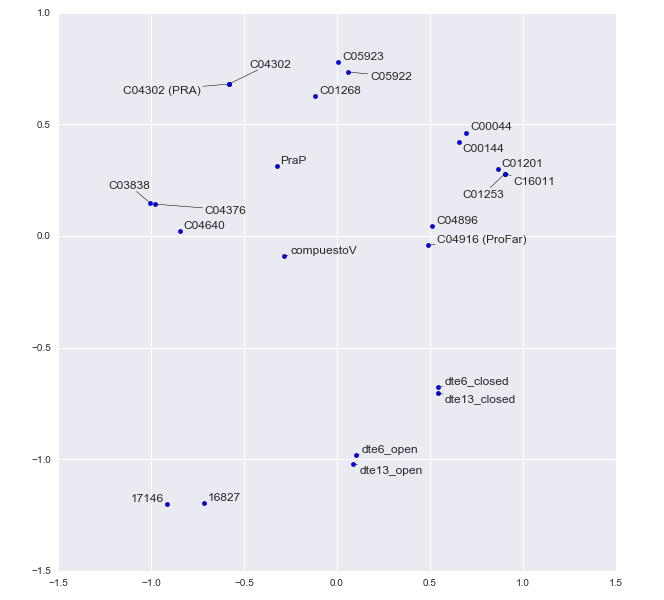
\includegraphics[angle = 0,scale = 0.6]{chapter4/SubstratesClustering.png}
  \caption[Substrates clustering according to Tanimoto distance]{\normalsize{Substrates clustering according to Tanimoto distance}}
  \label{fig:Substrates Tanimoto distance}
  \end{figure}
  
  On next figure we can see their chemical structures.
  
  \clearpage   
  
  \begin{figure}[h!tbp]
   \centering
   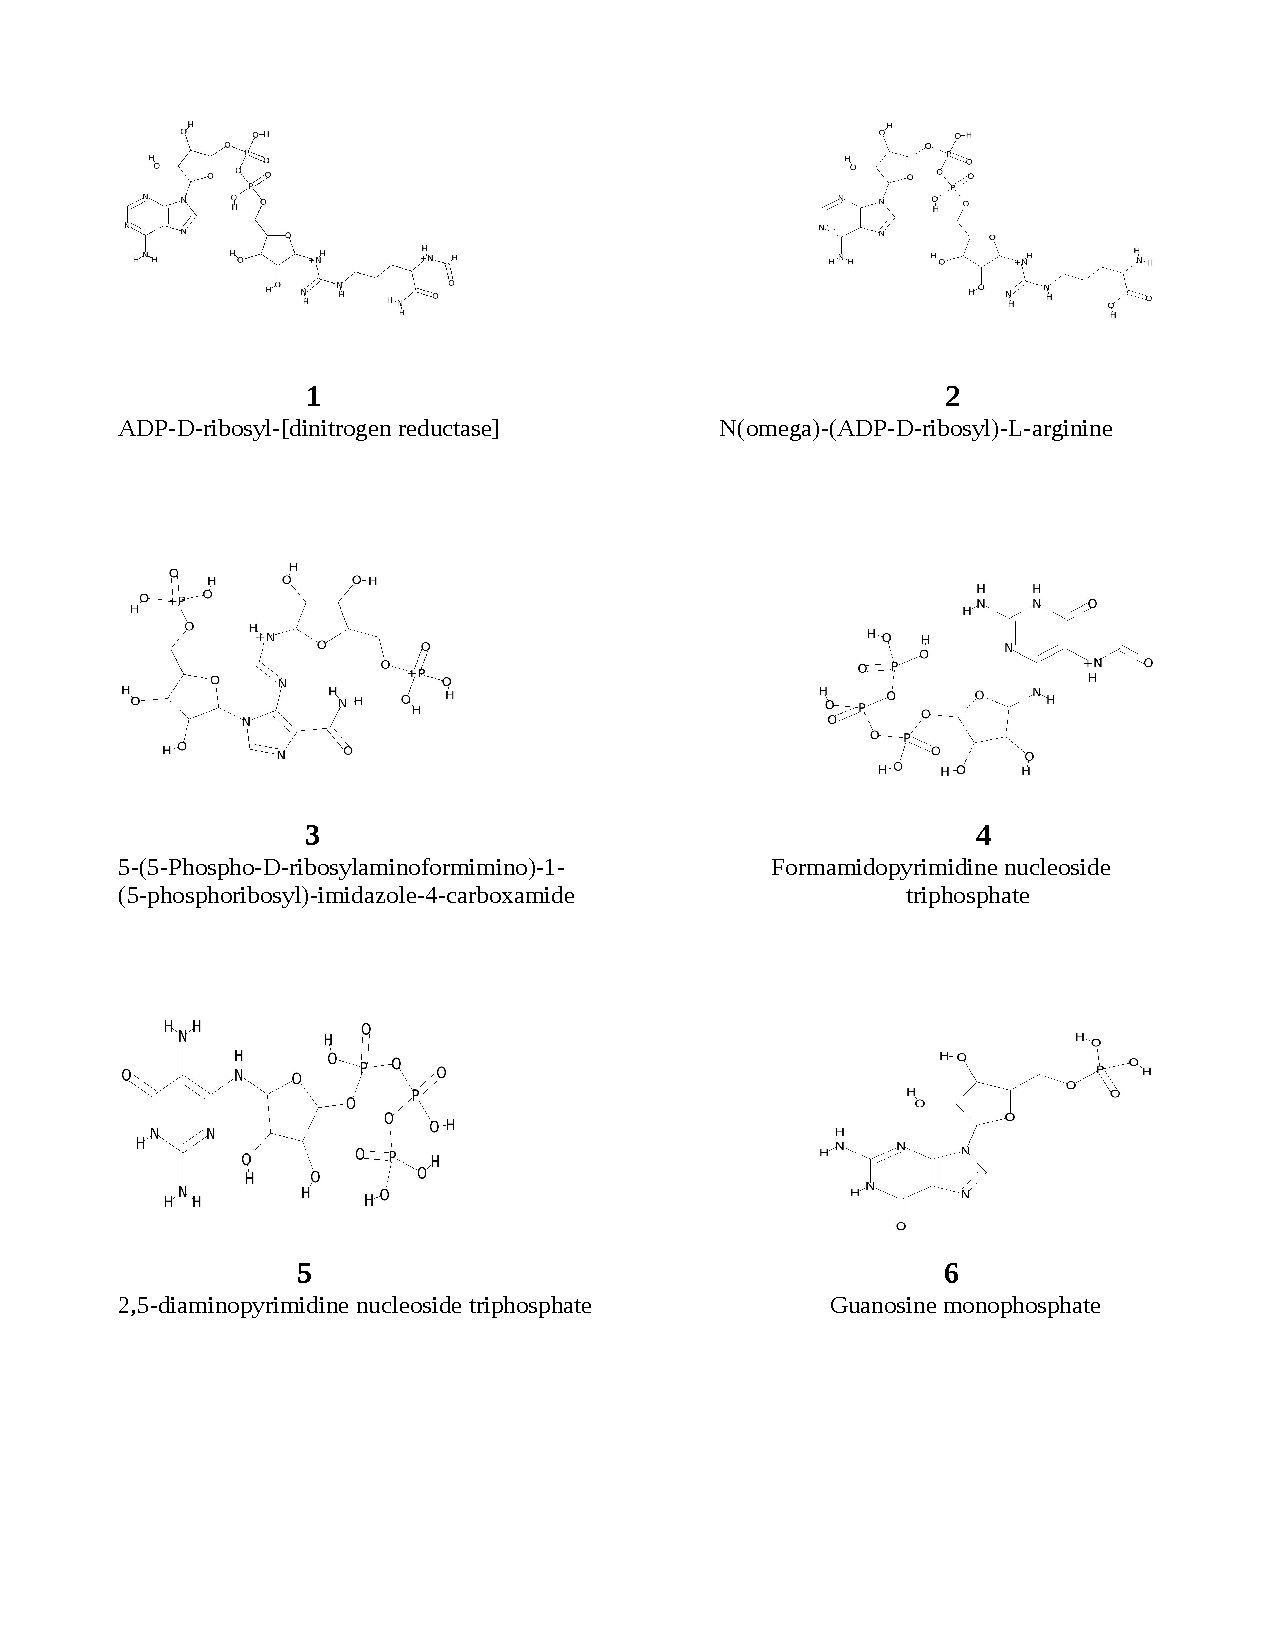
\includegraphics[angle = 0,scale = 1]{chapter4/esquema_quimico-1-1.pdf}
   \caption[Substrates 1]{\normalsize{Substrates 1}}
   \label{fig:Substrates chemical 1}
   \end{figure}
  
  \begin{figure}[h!tbp]
   \centering
   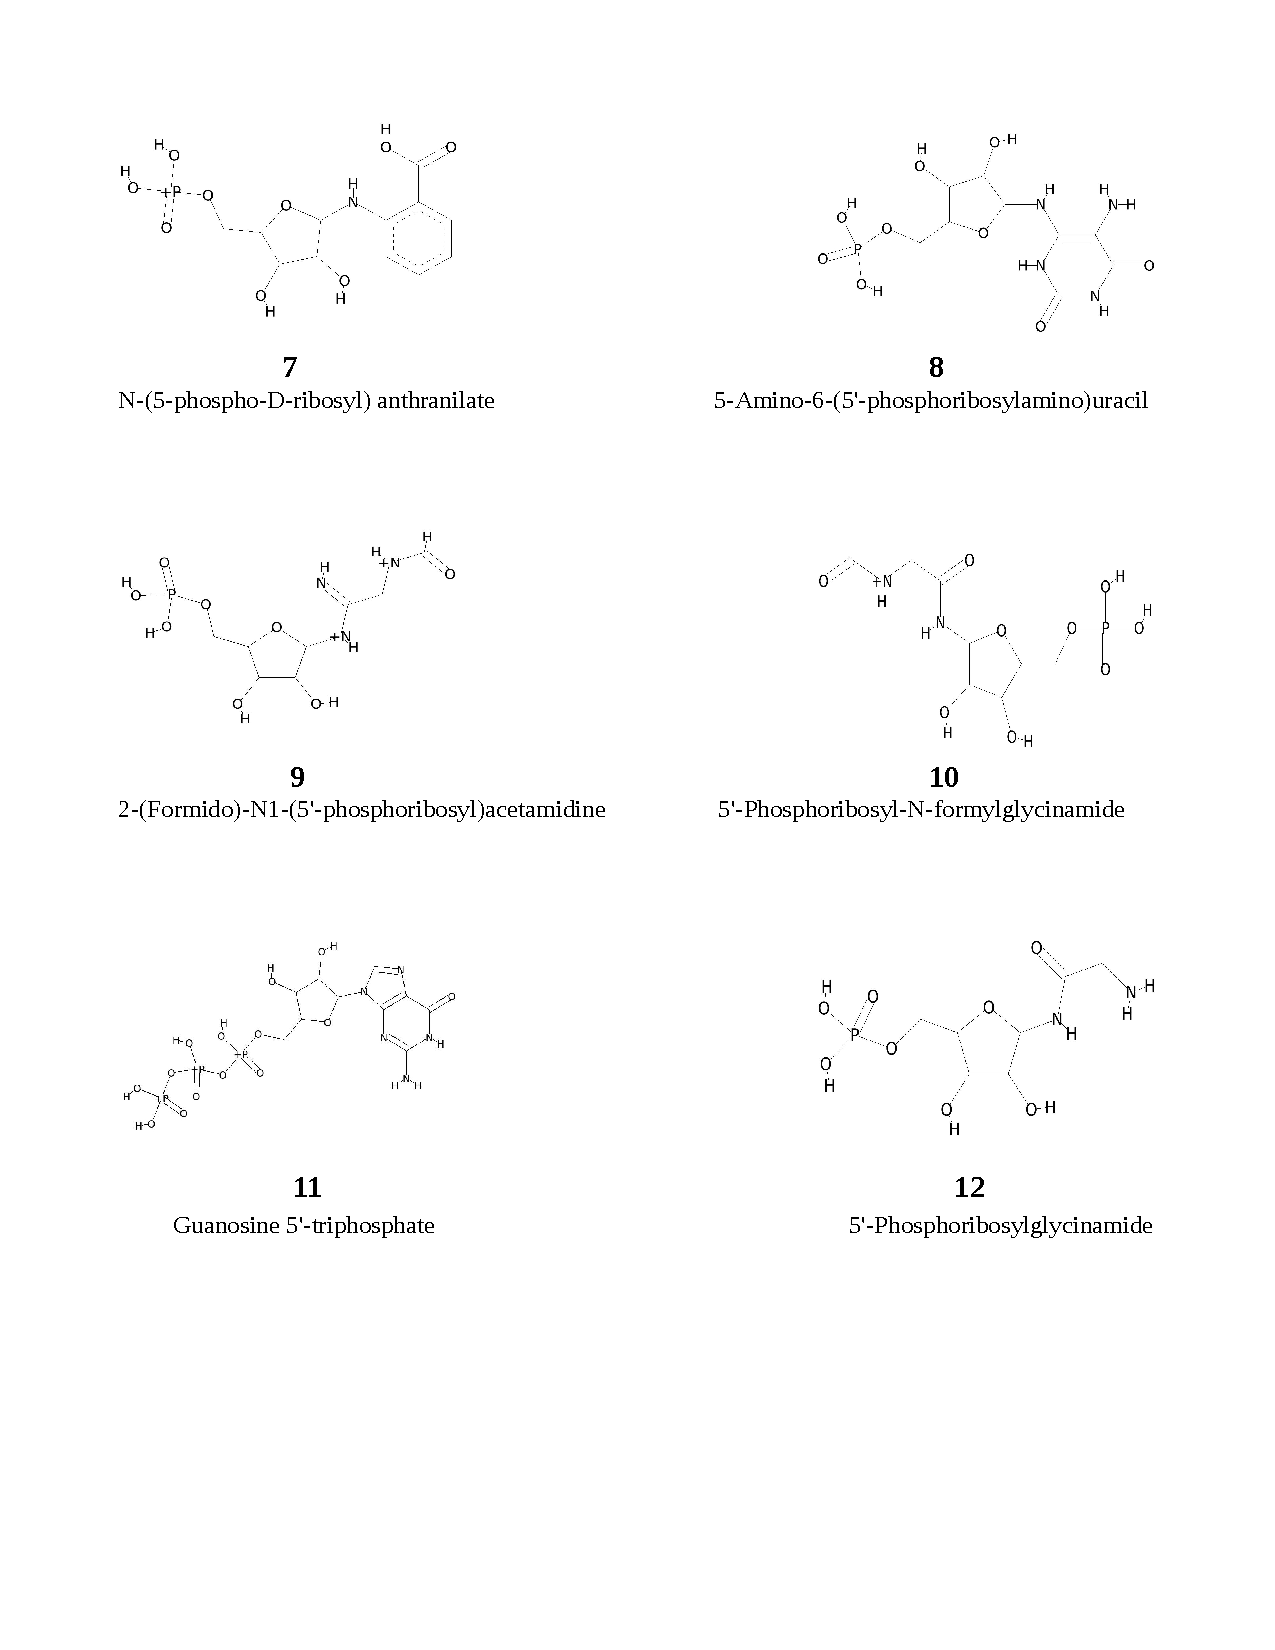
\includegraphics[angle = 0,scale = 1]{chapter4/esquema_quimico-2-2.pdf}
   \caption[Substrates 2]{\normalsize{Substrates 2}}
   \label{fig:Substrates chemical 2}
   \end{figure}
  
  \begin{figure}[h!tbp]
   \centering
   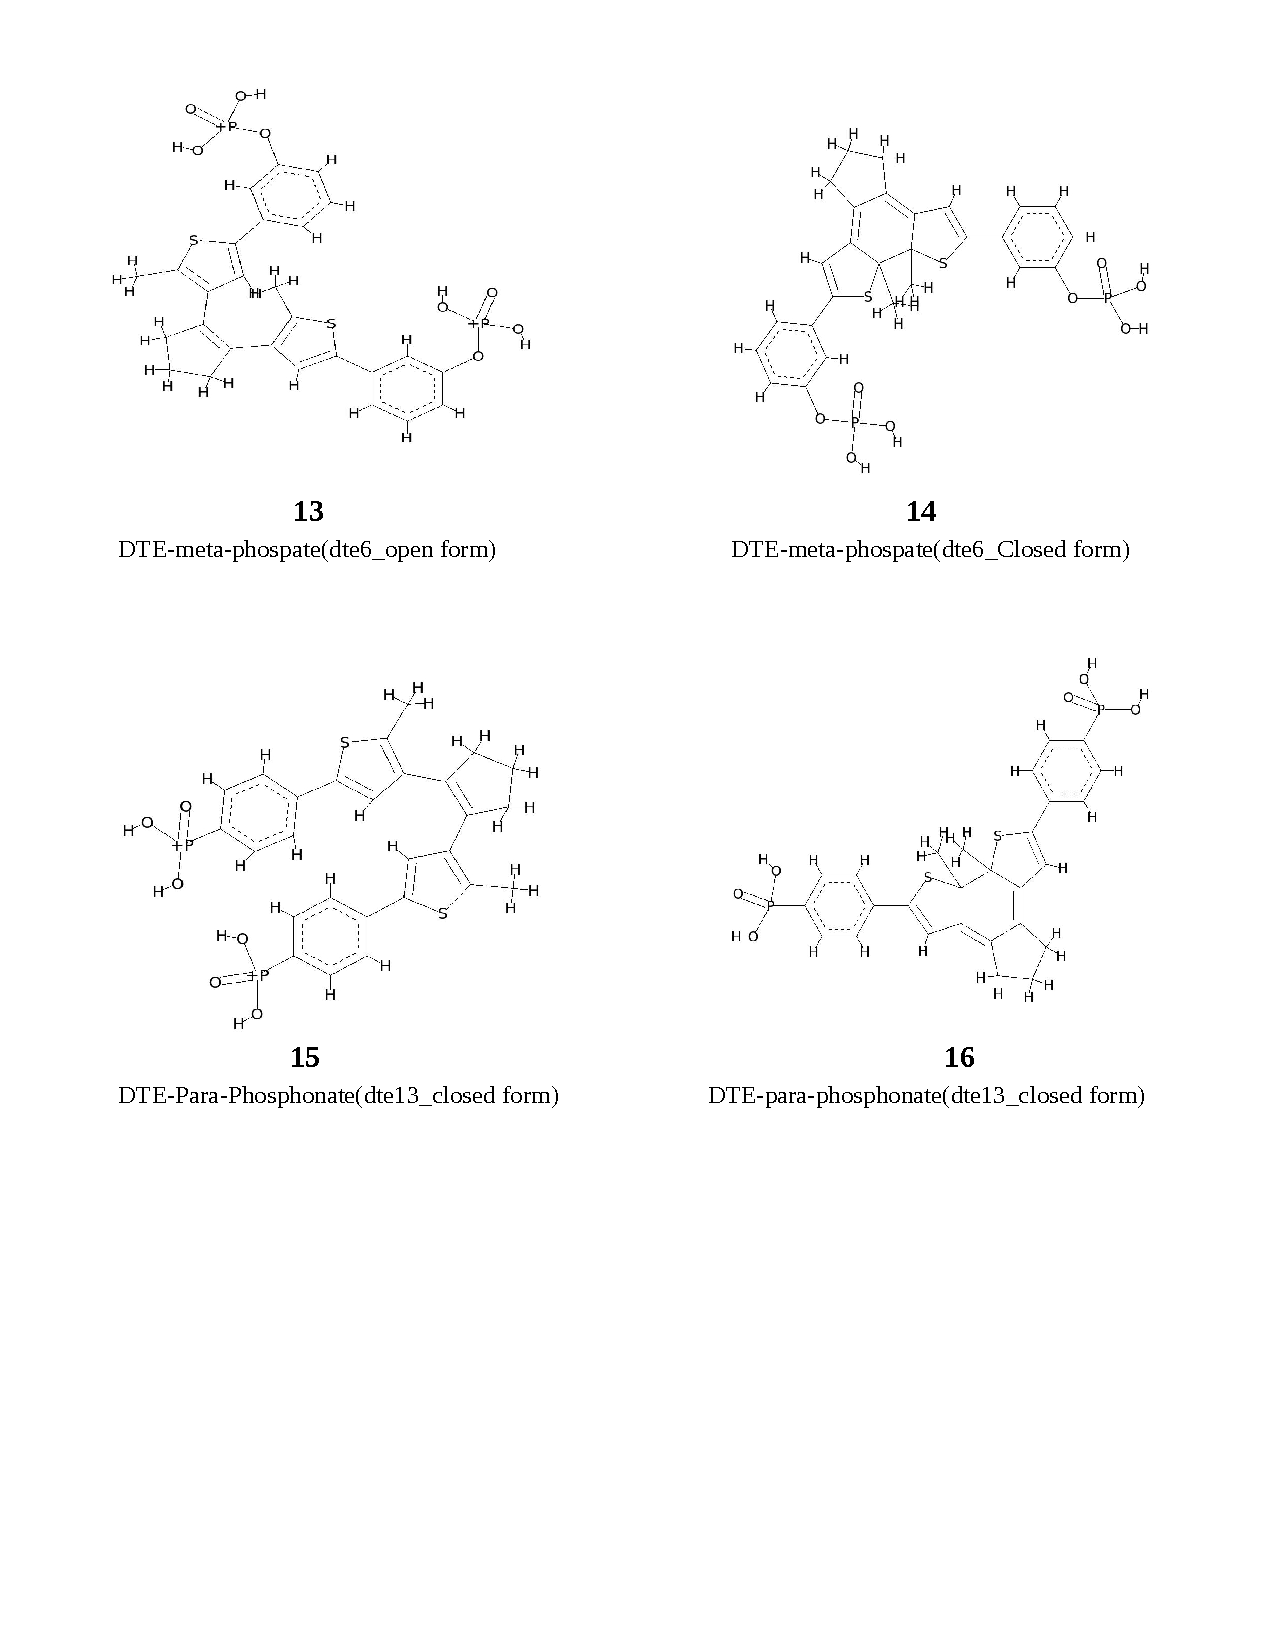
\includegraphics[angle = 0,scale = 1]{chapter4/esquema_quimico-3-3.pdf}
   \caption[Substrates 3]{\normalsize{Substrates 3}}
   \label{fig:Substrates chemical 3}
   \end{figure}
  
  \begin{figure}[h!tbp]
   \centering
   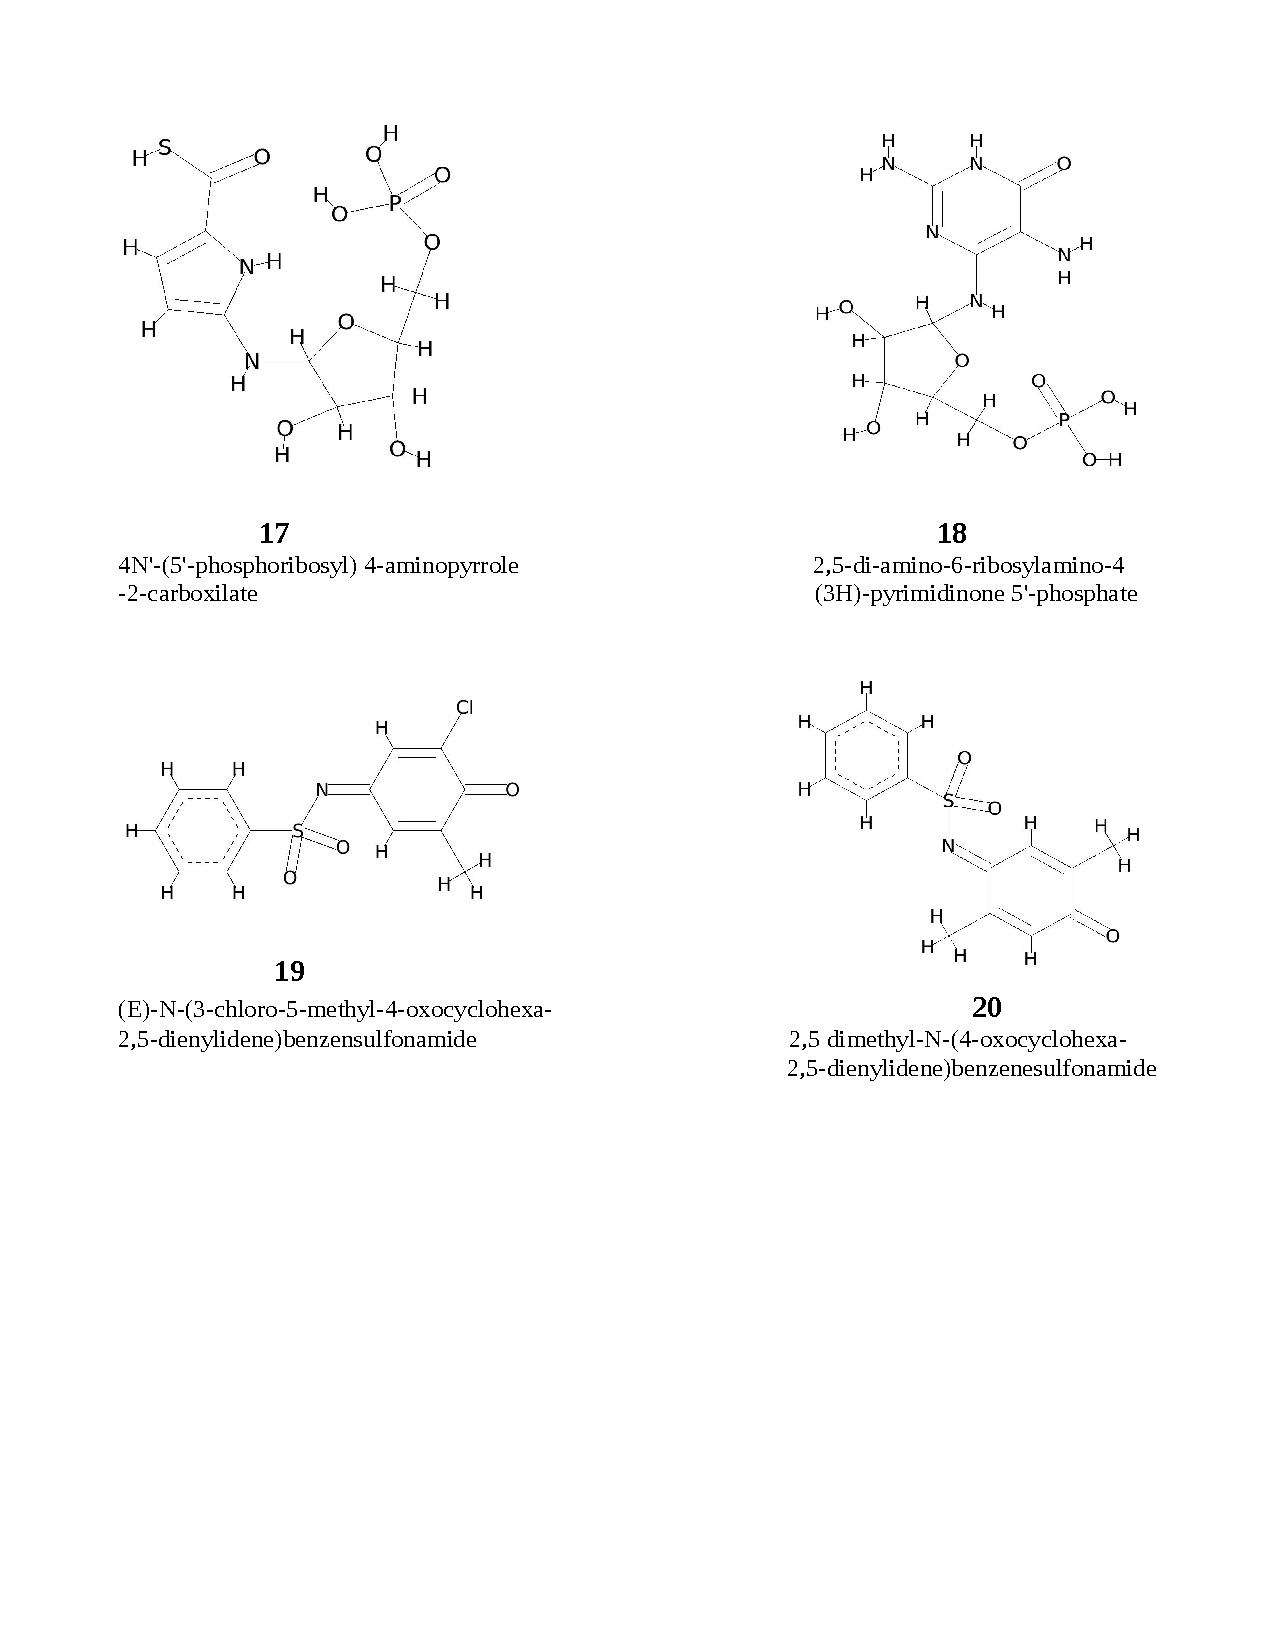
\includegraphics[angle = 0,scale = 1]{chapter4/esquema_quimico-4-4.pdf}
   \caption[Substrates 4]{\normalsize{Substrates 4}}
   \label{fig:Substrates chemical 4}
   \end{figure}
  
  \section{Docking between PriA enzymes and selected
  substrates}\label{docking-between-pria-enzymes-and-selected-substrates}
  
  Docking simulation were calculated for PriA \emph{Streptomyces} enzymes.
  TrpF enzymes from \emph{Streptomyces Mg1, Jonesia denitrificans, were
  added as controls}
  
  Procedures can be found at
  \href{https://github.com/tripplab/Docking/wiki}{Docking Protocols}
  
  \begin{Shaded}
  \begin{Highlighting}[]
  \NormalTok{docking <-}\StringTok{ }\KeywordTok{read.csv}\NormalTok{(}\StringTok{"chapter4/SmallHeat.data"}\NormalTok{, }\DataTypeTok{header=}\OtherTok{TRUE}\NormalTok{, }\DataTypeTok{sep=}\StringTok{"}\CharTok{\textbackslash{}t}\StringTok{"}\NormalTok{)}
  
  \ControlFlowTok{for}\NormalTok{ (i }\ControlFlowTok{in} \DecValTok{2}\OperatorTok{:}\DecValTok{21}\NormalTok{)}
  \NormalTok{\{}\KeywordTok{plot}\NormalTok{(}\KeywordTok{density}\NormalTok{(docking[,i],}\DataTypeTok{na.rm=}\NormalTok{T)); }\KeywordTok{rug}\NormalTok{(docking[,i]);}\KeywordTok{browser}\NormalTok{()\}}
  \end{Highlighting}
  \end{Shaded}
  
  \begin{center}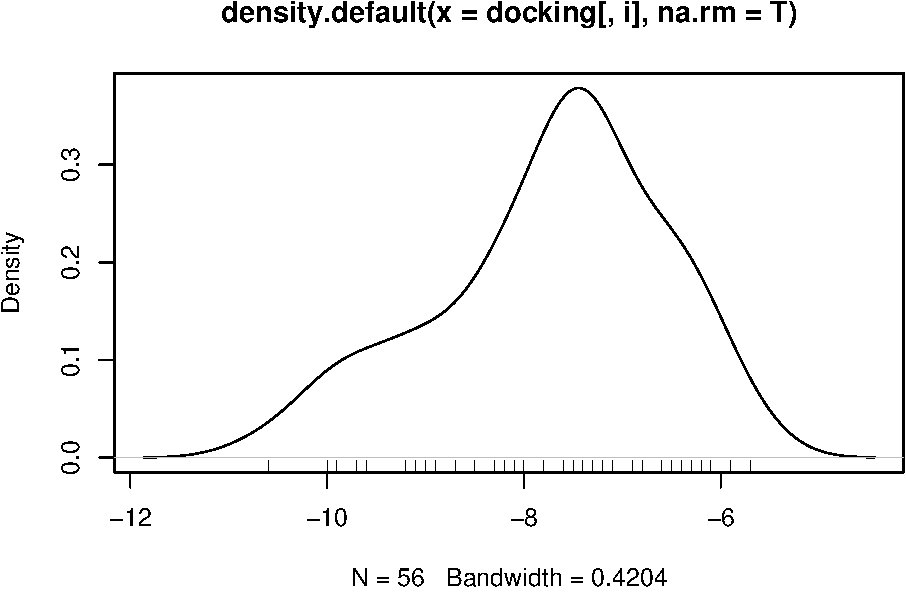
\includegraphics{tesis_files/figure-latex/johan-1} \end{center}
  
  \begin{verbatim}
  Called from: eval(expr, envir, enclos)
  debug en <text>#4: plot(density(docking[, i], na.rm = T))
  \end{verbatim}
  
  \begin{center}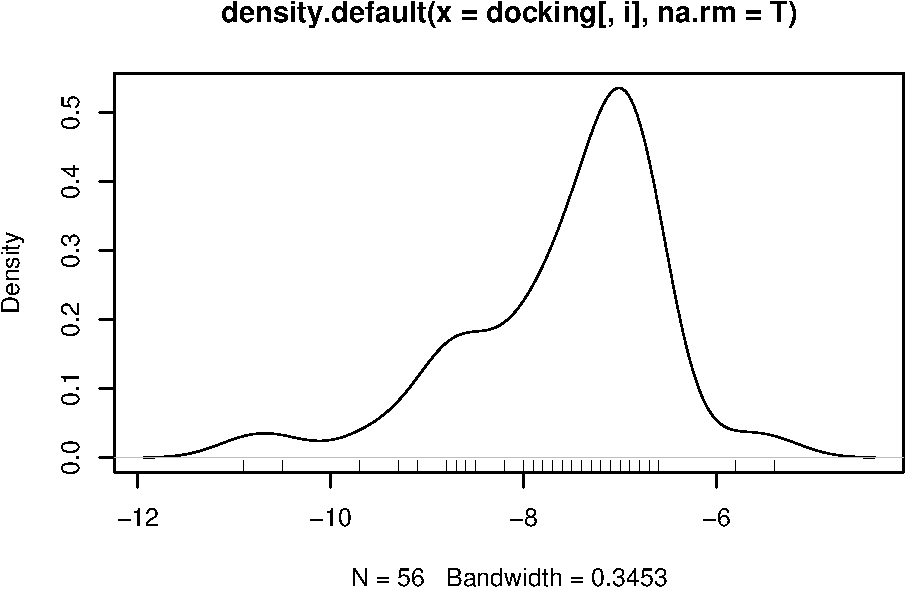
\includegraphics{tesis_files/figure-latex/johan-2} \end{center}
  
  \begin{verbatim}
  debug en <text>#4: rug(docking[, i])
  debug en <text>#4: browser()
  debug en <text>#4: plot(density(docking[, i], na.rm = T))
  \end{verbatim}
  
  \begin{center}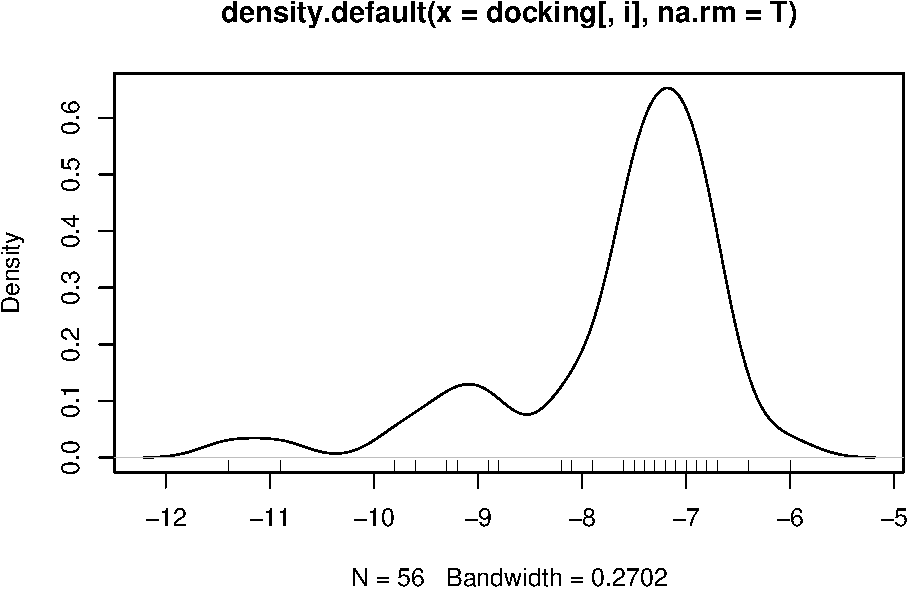
\includegraphics{tesis_files/figure-latex/johan-3} \end{center}
  
  \begin{verbatim}
  debug en <text>#4: rug(docking[, i])
  debug en <text>#4: browser()
  debug en <text>#4: plot(density(docking[, i], na.rm = T))
  \end{verbatim}
  
  \begin{center}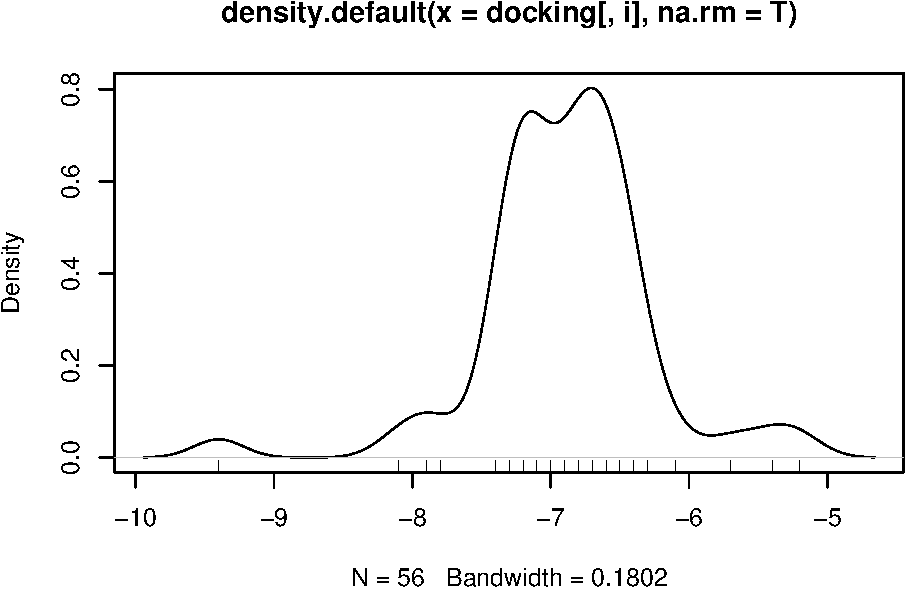
\includegraphics{tesis_files/figure-latex/johan-4} \end{center}
  
  \begin{verbatim}
  debug en <text>#4: rug(docking[, i])
  debug en <text>#4: browser()
  debug en <text>#4: plot(density(docking[, i], na.rm = T))
  \end{verbatim}
  
  \begin{center}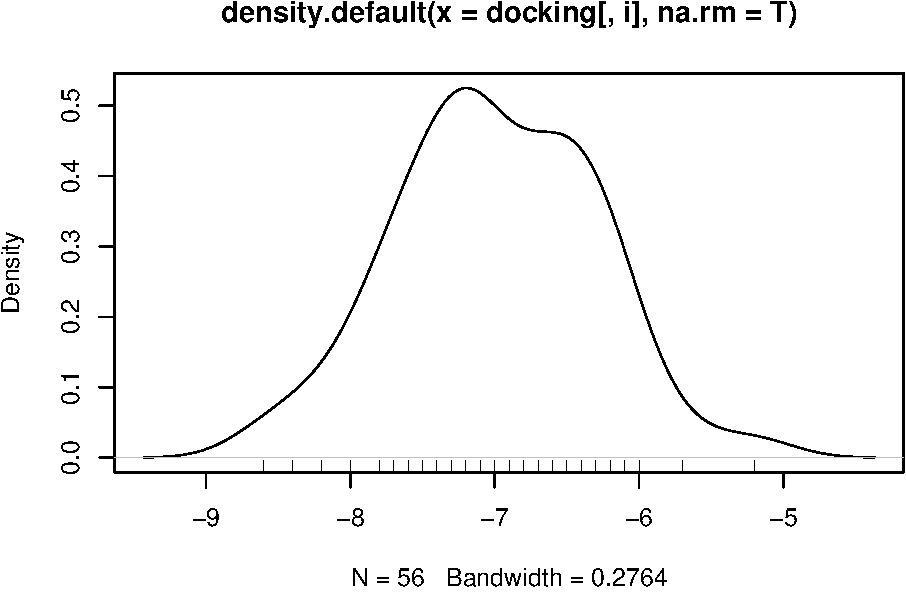
\includegraphics{tesis_files/figure-latex/johan-5} \end{center}
  
  \begin{verbatim}
  debug en <text>#4: rug(docking[, i])
  debug en <text>#4: browser()
  debug en <text>#4: plot(density(docking[, i], na.rm = T))
  \end{verbatim}
  
  \begin{center}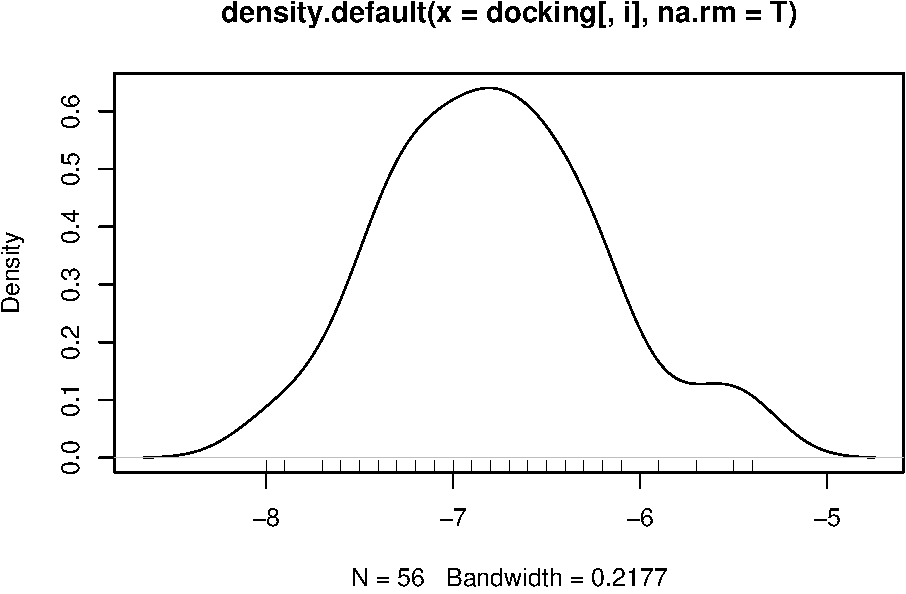
\includegraphics{tesis_files/figure-latex/johan-6} \end{center}
  
  \begin{verbatim}
  debug en <text>#4: rug(docking[, i])
  debug en <text>#4: browser()
  debug en <text>#4: plot(density(docking[, i], na.rm = T))
  \end{verbatim}
  
  \begin{center}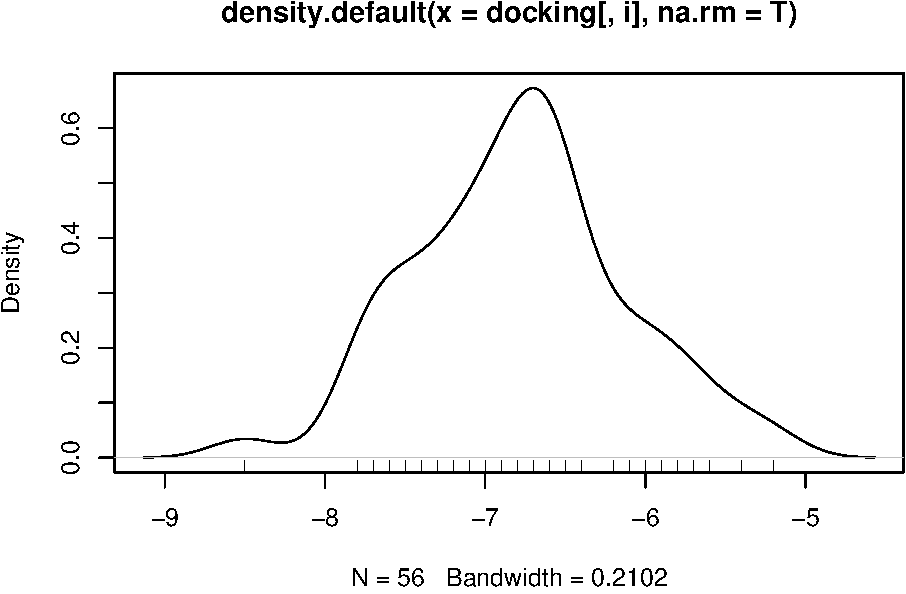
\includegraphics{tesis_files/figure-latex/johan-7} \end{center}
  
  \begin{verbatim}
  debug en <text>#4: rug(docking[, i])
  debug en <text>#4: browser()
  debug en <text>#4: plot(density(docking[, i], na.rm = T))
  \end{verbatim}
  
  \begin{center}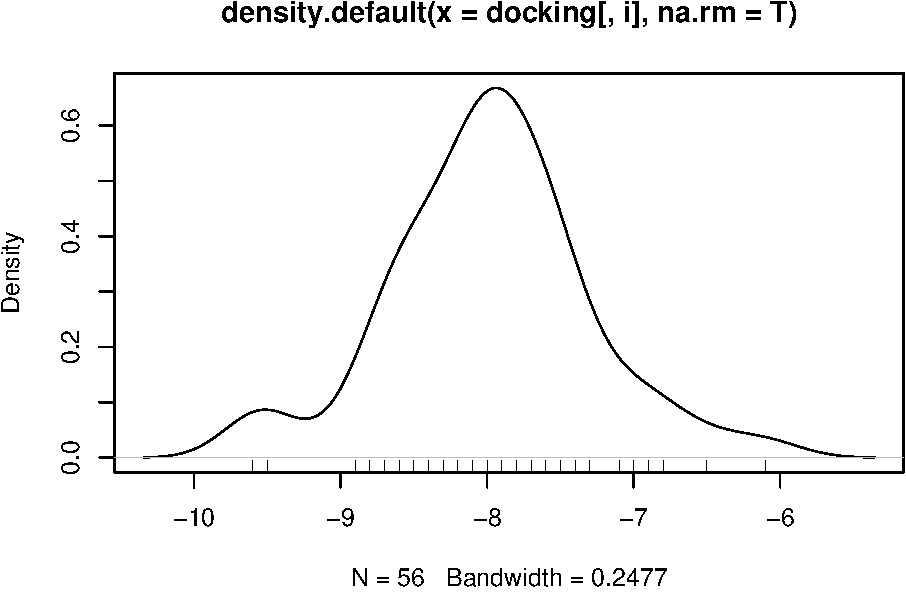
\includegraphics{tesis_files/figure-latex/johan-8} \end{center}
  
  \begin{verbatim}
  debug en <text>#4: rug(docking[, i])
  debug en <text>#4: browser()
  debug en <text>#4: plot(density(docking[, i], na.rm = T))
  \end{verbatim}
  
  \begin{center}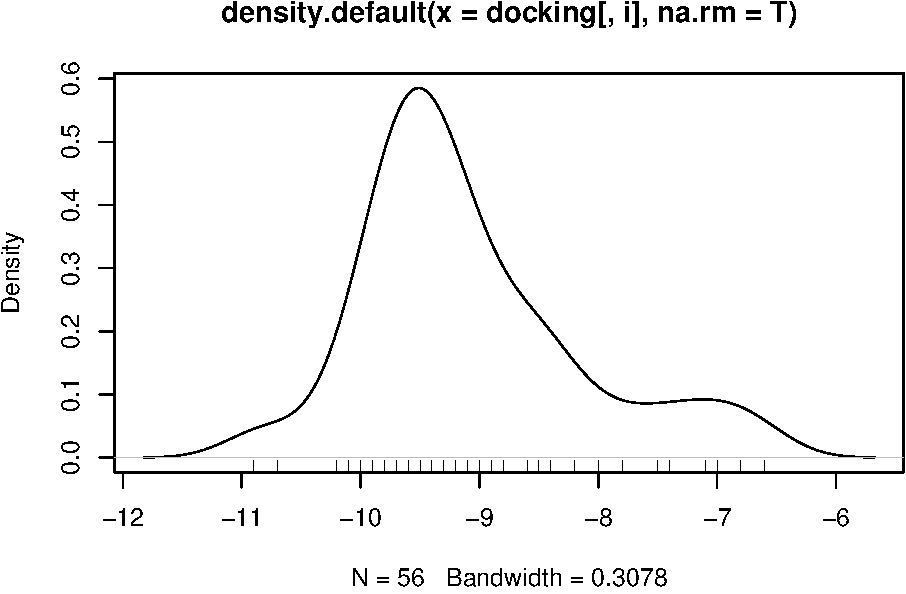
\includegraphics{tesis_files/figure-latex/johan-9} \end{center}
  
  \begin{verbatim}
  debug en <text>#4: rug(docking[, i])
  debug en <text>#4: browser()
  debug en <text>#4: plot(density(docking[, i], na.rm = T))
  \end{verbatim}
  
  \begin{center}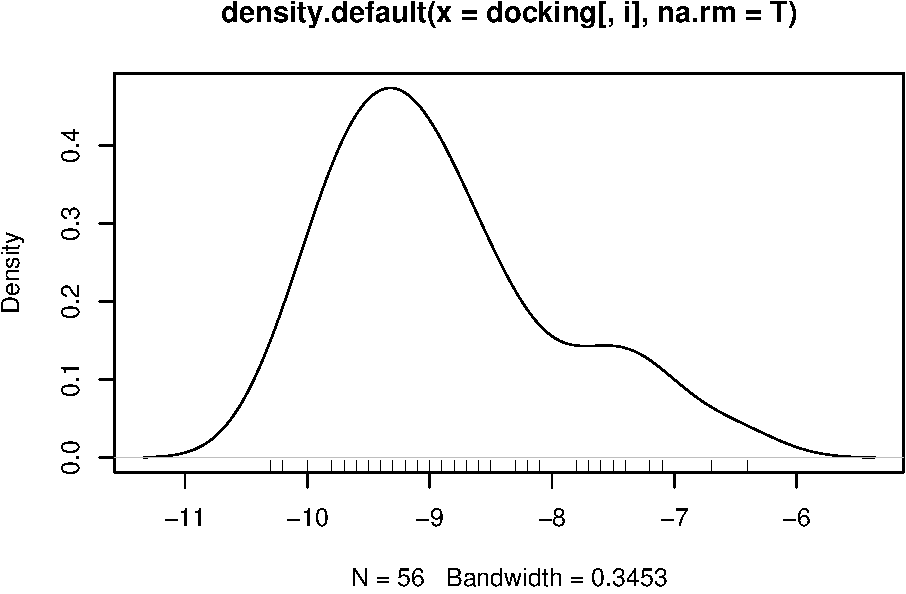
\includegraphics{tesis_files/figure-latex/johan-10} \end{center}
  
  \begin{verbatim}
  debug en <text>#4: rug(docking[, i])
  debug en <text>#4: browser()
  debug en <text>#4: plot(density(docking[, i], na.rm = T))
  \end{verbatim}
  
  \begin{center}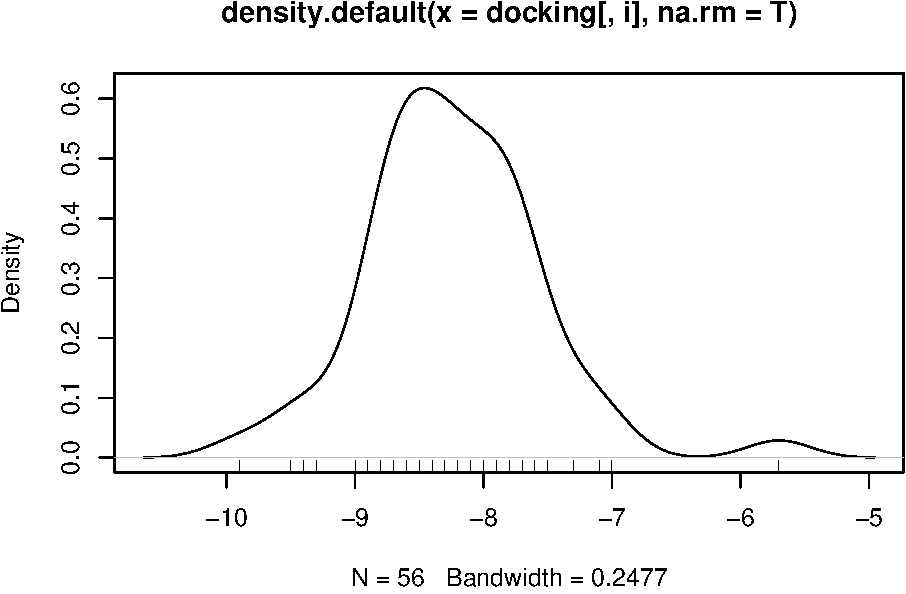
\includegraphics{tesis_files/figure-latex/johan-11} \end{center}
  
  \begin{verbatim}
  debug en <text>#4: rug(docking[, i])
  debug en <text>#4: browser()
  debug en <text>#4: plot(density(docking[, i], na.rm = T))
  \end{verbatim}
  
  \begin{center}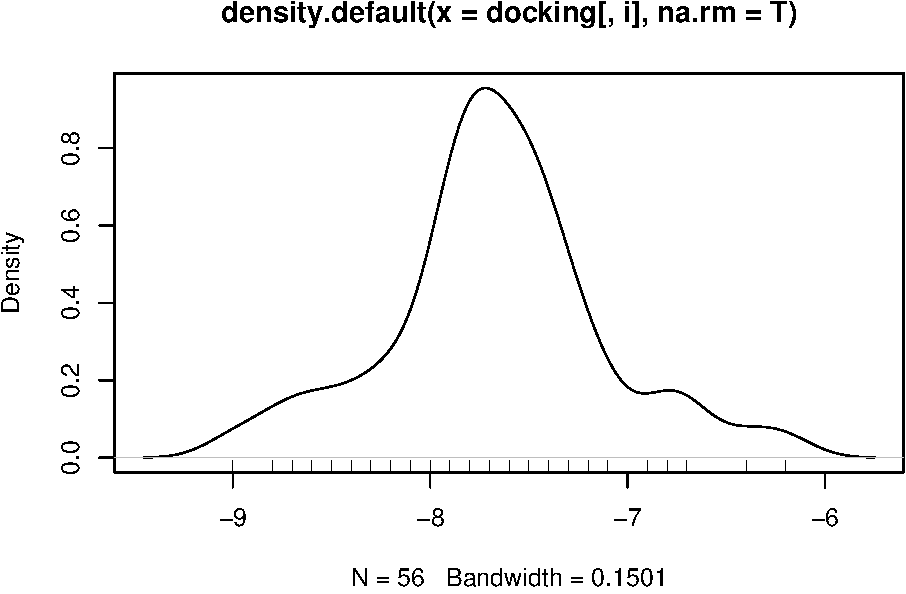
\includegraphics{tesis_files/figure-latex/johan-12} \end{center}
  
  \begin{verbatim}
  debug en <text>#4: rug(docking[, i])
  debug en <text>#4: browser()
  debug en <text>#4: plot(density(docking[, i], na.rm = T))
  \end{verbatim}
  
  \begin{center}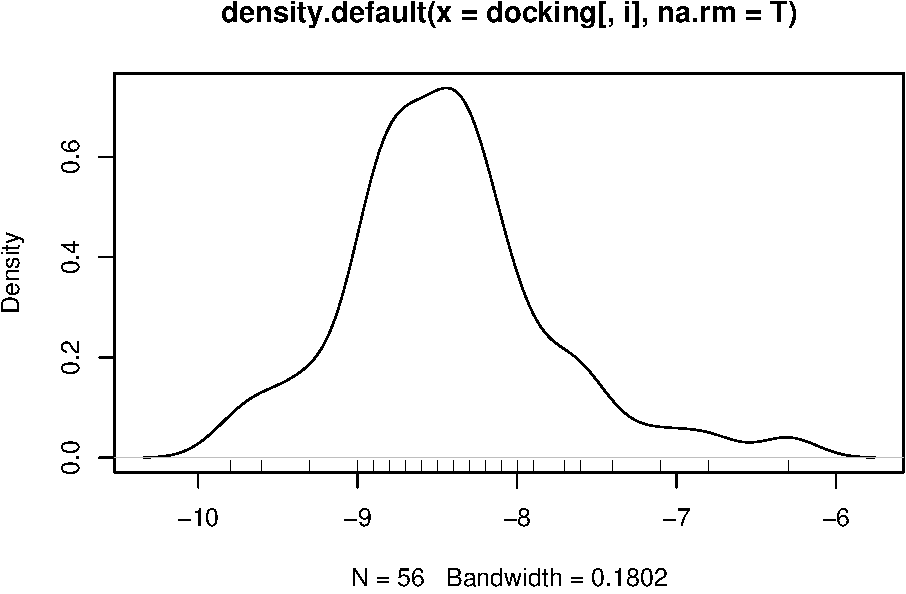
\includegraphics{tesis_files/figure-latex/johan-13} \end{center}
  
  \begin{verbatim}
  debug en <text>#4: rug(docking[, i])
  debug en <text>#4: browser()
  debug en <text>#4: plot(density(docking[, i], na.rm = T))
  \end{verbatim}
  
  \begin{center}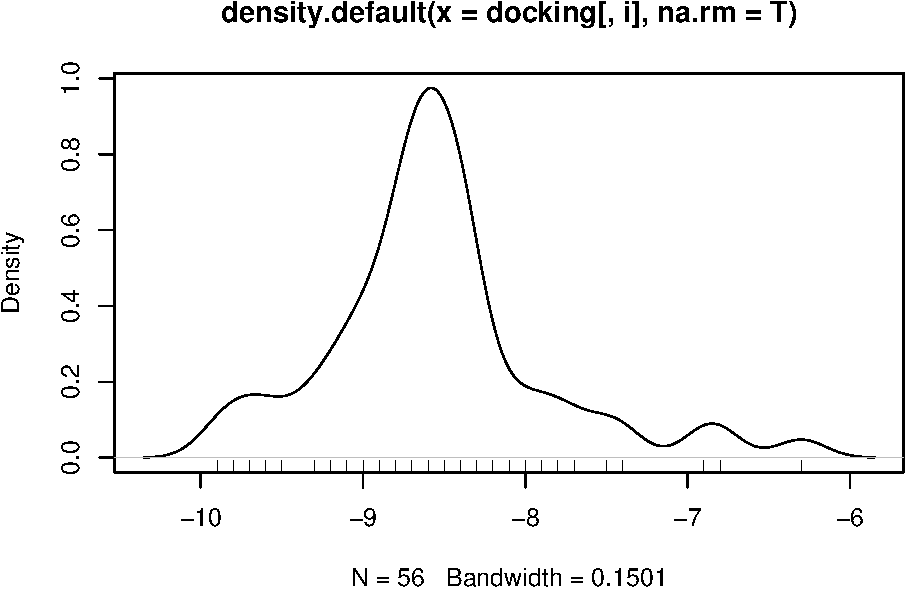
\includegraphics{tesis_files/figure-latex/johan-14} \end{center}
  
  \begin{verbatim}
  debug en <text>#4: rug(docking[, i])
  debug en <text>#4: browser()
  debug en <text>#4: plot(density(docking[, i], na.rm = T))
  \end{verbatim}
  
  \begin{center}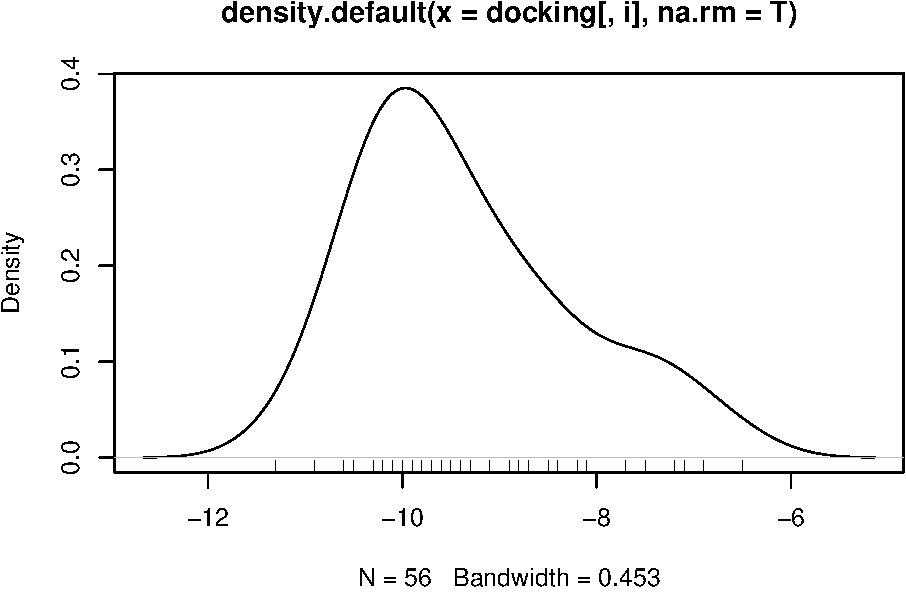
\includegraphics{tesis_files/figure-latex/johan-15} \end{center}
  
  \begin{verbatim}
  debug en <text>#4: rug(docking[, i])
  debug en <text>#4: browser()
  debug en <text>#4: plot(density(docking[, i], na.rm = T))
  \end{verbatim}
  
  \begin{center}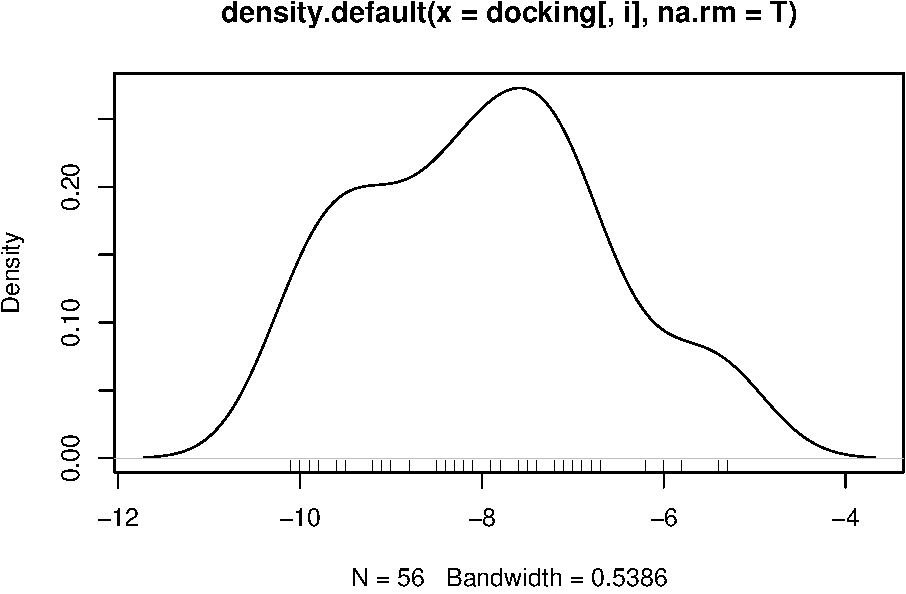
\includegraphics{tesis_files/figure-latex/johan-16} \end{center}
  
  \begin{verbatim}
  debug en <text>#4: rug(docking[, i])
  debug en <text>#4: browser()
  debug en <text>#4: plot(density(docking[, i], na.rm = T))
  \end{verbatim}
  
  \begin{center}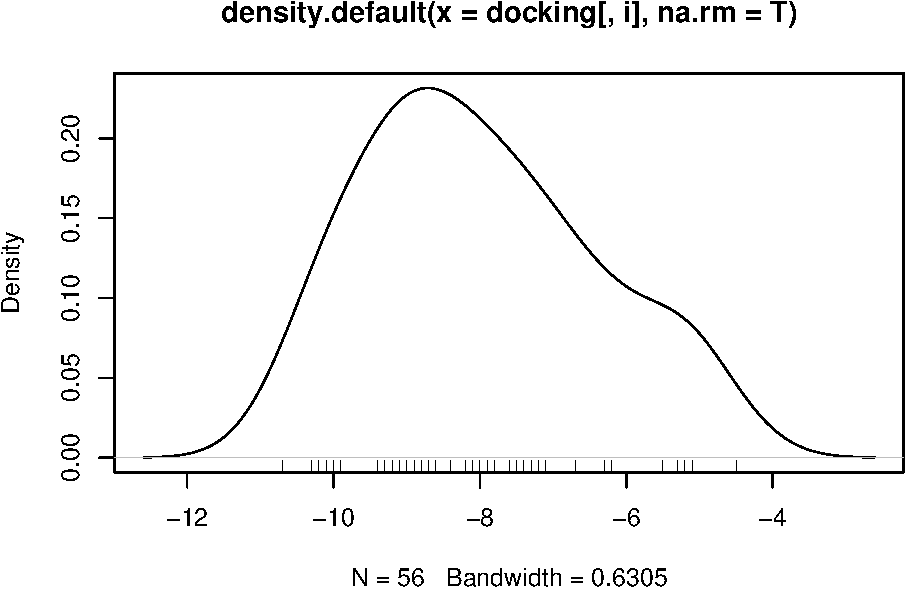
\includegraphics{tesis_files/figure-latex/johan-17} \end{center}
  
  \begin{verbatim}
  debug en <text>#4: rug(docking[, i])
  debug en <text>#4: browser()
  debug en <text>#4: plot(density(docking[, i], na.rm = T))
  \end{verbatim}
  
  \begin{center}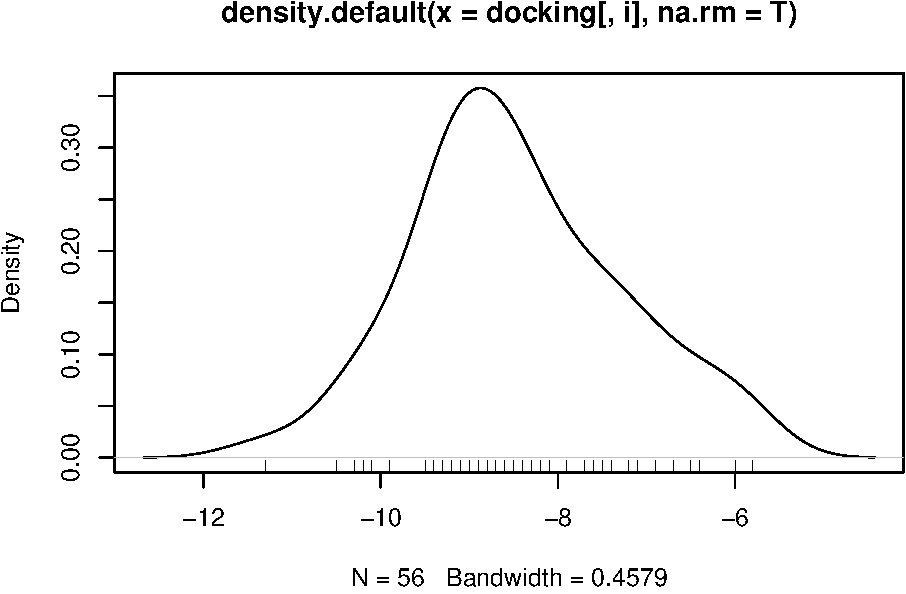
\includegraphics{tesis_files/figure-latex/johan-18} \end{center}
  
  \begin{verbatim}
  debug en <text>#4: rug(docking[, i])
  debug en <text>#4: browser()
  debug en <text>#4: plot(density(docking[, i], na.rm = T))
  \end{verbatim}
  
  \begin{center}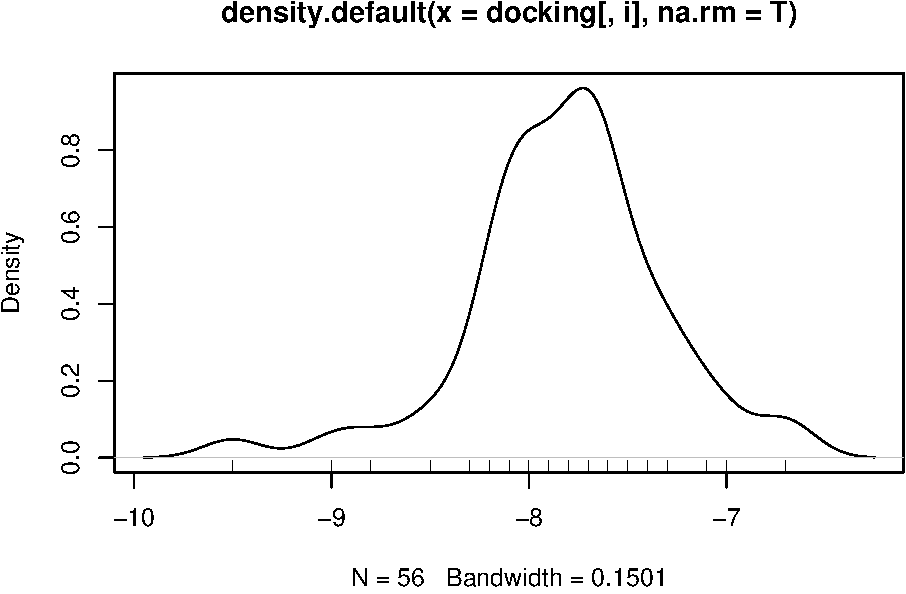
\includegraphics{tesis_files/figure-latex/johan-19} \end{center}
  
  \begin{verbatim}
  debug en <text>#4: rug(docking[, i])
  debug en <text>#4: browser()
  debug en <text>#4: plot(density(docking[, i], na.rm = T))
  \end{verbatim}
  
  \begin{center}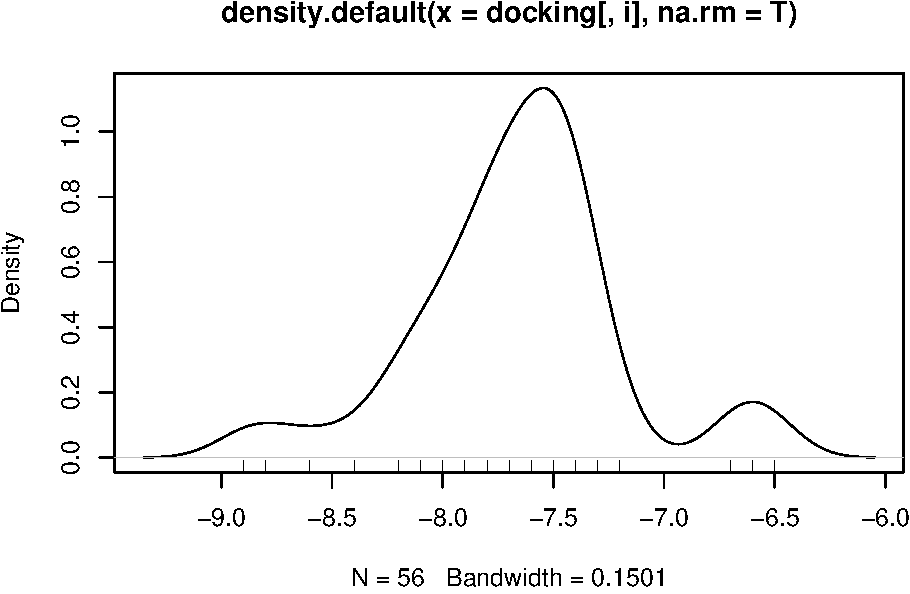
\includegraphics{tesis_files/figure-latex/johan-20} \end{center}
  
  \begin{verbatim}
  debug en <text>#4: rug(docking[, i])
  debug en <text>#4: browser()
  \end{verbatim}
  
  \begin{Shaded}
  \begin{Highlighting}[]
  \KeywordTok{plot}\NormalTok{(}\KeywordTok{cor}\NormalTok{(docking[}\OperatorTok{-}\KeywordTok{c}\NormalTok{(}\DecValTok{5}\NormalTok{,}\DecValTok{12}\NormalTok{,}\DecValTok{13}\NormalTok{,}\DecValTok{38}\NormalTok{,}\DecValTok{51}\NormalTok{),}\OperatorTok{-}\DecValTok{1}\NormalTok{]))}
  \end{Highlighting}
  \end{Shaded}
  
  \begin{center}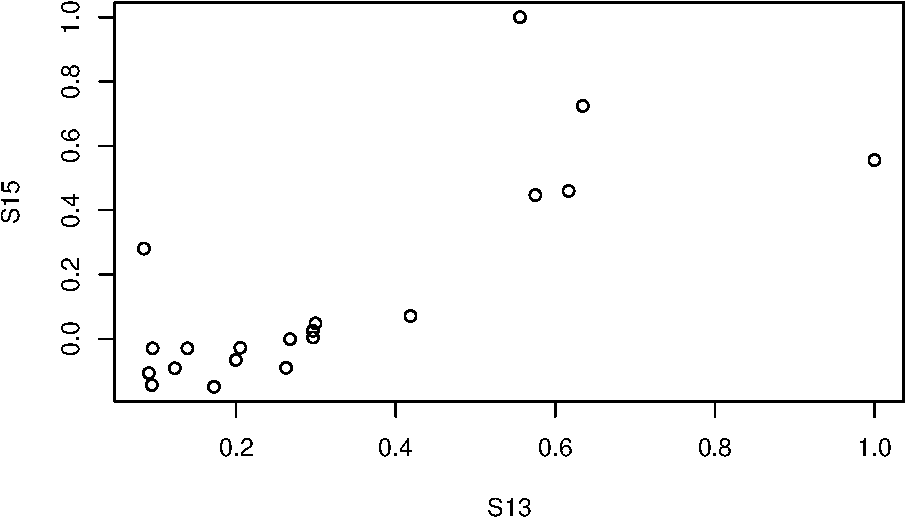
\includegraphics{tesis_files/figure-latex/johan-21} \end{center}
  
  \begin{Shaded}
  \begin{Highlighting}[]
  \NormalTok{## Leer sobre la incertidumbre del 2 y explicarla  }
  \NormalTok{## Y leer el paper de Julian y el de mauricio sobre reportes de docking}
  \end{Highlighting}
  \end{Shaded}
  
  \begin{Shaded}
  \begin{Highlighting}[]
  \KeywordTok{ggplot}\NormalTok{(docking.m, }\KeywordTok{aes}\NormalTok{(}\DataTypeTok{x=}\NormalTok{variable, }\DataTypeTok{y=}\NormalTok{Enzima)) }\OperatorTok{+}\StringTok{ }\KeywordTok{labs}\NormalTok{(}\DataTypeTok{x =} \StringTok{"Substrates"}\NormalTok{, }\DataTypeTok{y =} \StringTok{"Enzymes"}\NormalTok{,}\DataTypeTok{text =} \KeywordTok{element_text}\NormalTok{(}\DataTypeTok{size=}\DecValTok{12}\NormalTok{))}\OperatorTok{+}\StringTok{ }\KeywordTok{scale_fill_gradientn}\NormalTok{(}\DataTypeTok{colours =} \KeywordTok{hm.palette}\NormalTok{(}\DecValTok{100}\NormalTok{),}\DataTypeTok{na.value =} \StringTok{"gray"}\NormalTok{)}\OperatorTok{+}\KeywordTok{theme_bw}\NormalTok{()}\OperatorTok{+}\KeywordTok{theme}\NormalTok{(}\DataTypeTok{plot.title =} \KeywordTok{element_text}\NormalTok{(}\DataTypeTok{size =} \DecValTok{14}\NormalTok{, }\DataTypeTok{face =} \StringTok{"bold"}\NormalTok{), }\DataTypeTok{text =} \KeywordTok{element_text}\NormalTok{(}\DataTypeTok{size =} \DecValTok{12}\NormalTok{), }\DataTypeTok{axis.title =} \KeywordTok{element_text}\NormalTok{(}\DataTypeTok{face=}\StringTok{"bold"}\NormalTok{), }\DataTypeTok{axis.text.x=}\KeywordTok{element_text}\NormalTok{(}\DataTypeTok{angle =} \DecValTok{90}\NormalTok{,}\DataTypeTok{size =} \DecValTok{6}\NormalTok{))}
  \end{Highlighting}
  \end{Shaded}
  
  \begin{center}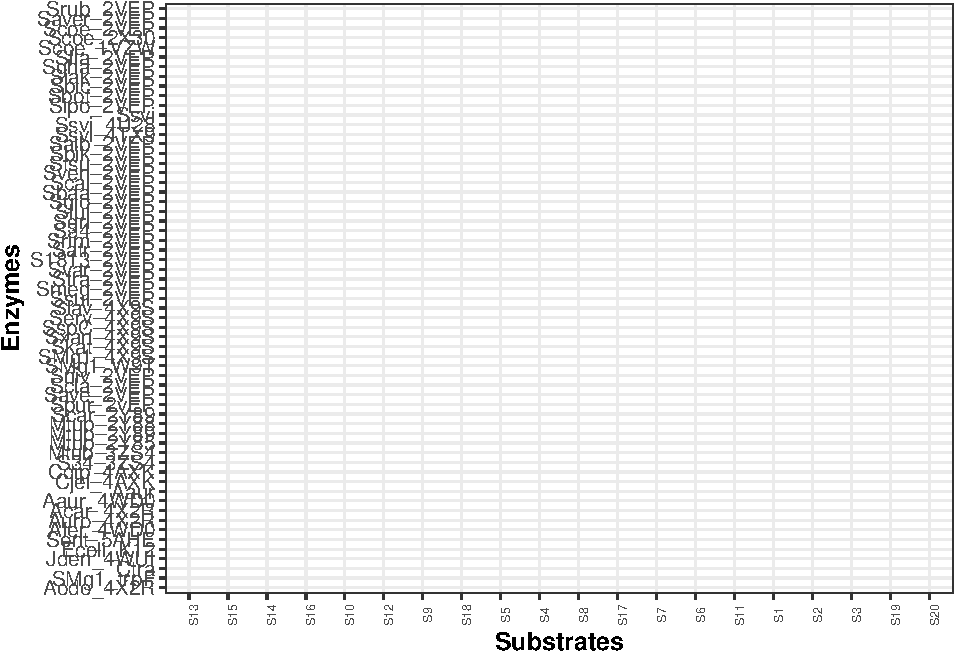
\includegraphics{tesis_files/figure-latex/heatonPDF-1} \end{center}
  
  \begin{figure}[h!tbp]
  \centering
  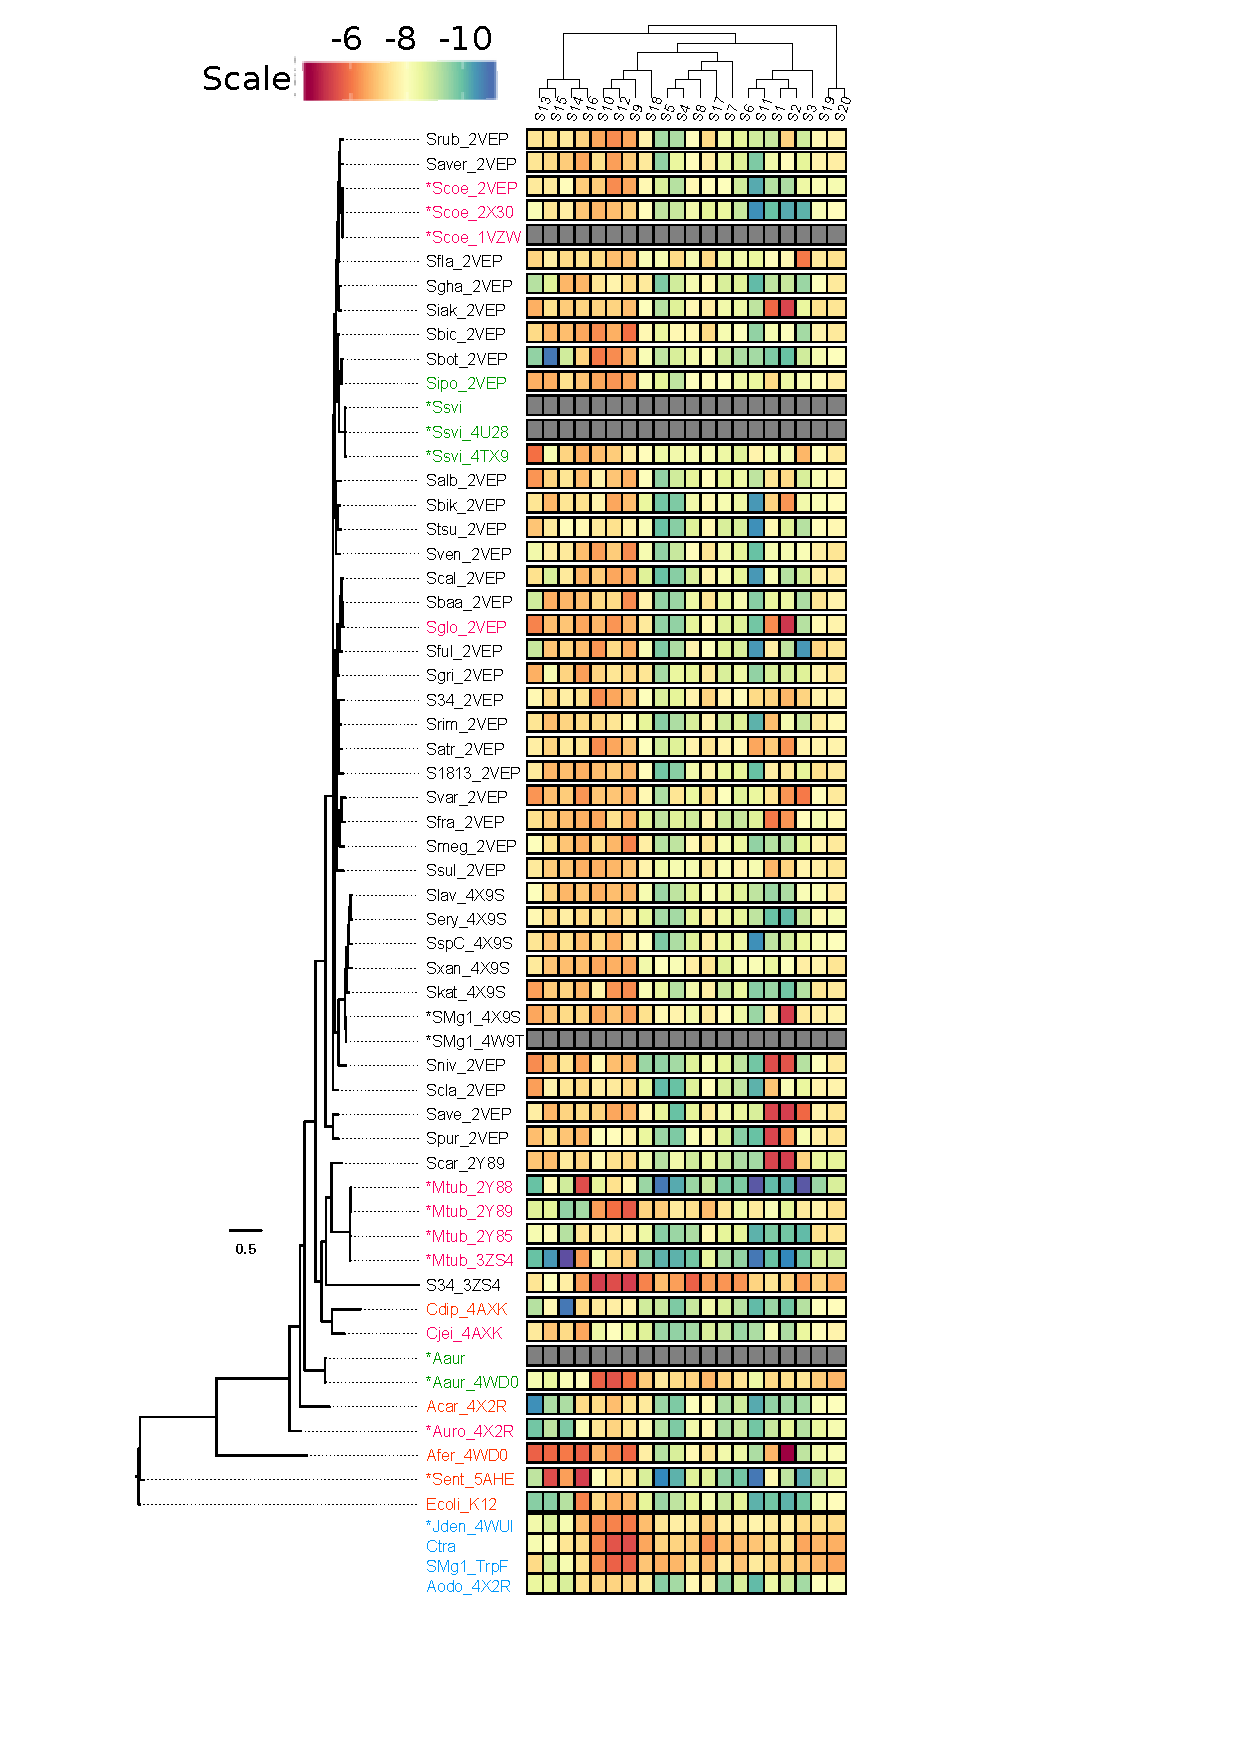
\includegraphics[angle = 0,scale = 1]{chapter4/Figura1_4.pdf}
  \caption[Heatplot docking PriA enzyme Family vs substrates]{\normalsize{Heatplot docking PriA enzyme Family vs substrates}}
  \label{fig:Heatplod PriA docking}
  \end{figure}
  
  \begin{figure}[h!tbp]
  \centering
  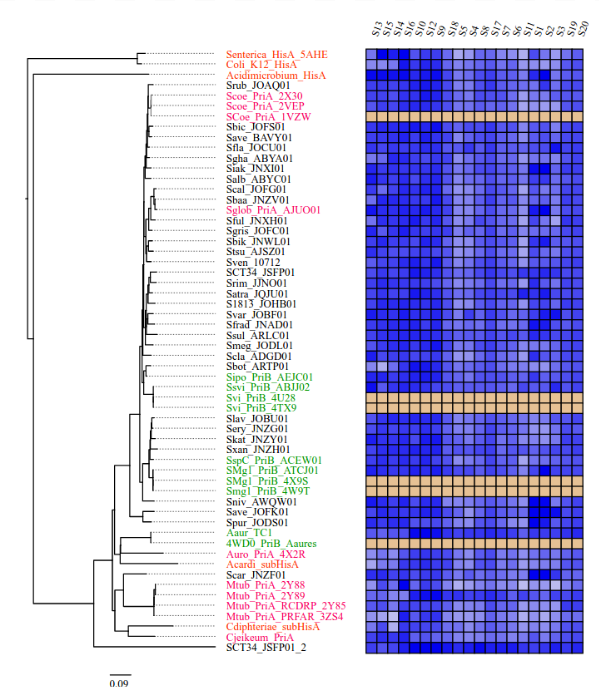
\includegraphics[angle = 0,scale = 0.6]{chapter4/PriAHeatPot.png}
  \caption[Heat Plot PriA Streptomyces vs other subtrates]{\normalsize{Heat Plot PriA Streptomyces vs other subtrates}}
  \label{fig:PriADocking}
  \end{figure}
  
  \section{GTP is the substrate with best PriA
  affinity}\label{gtp-is-the-substrate-with-best-pria-affinity}
  
  \begin{Shaded}
  \begin{Highlighting}[]
  \NormalTok{## boxplot de los sustratos}
  \KeywordTok{ggplot}\NormalTok{(docking.m, }\KeywordTok{aes}\NormalTok{(}\DataTypeTok{x=}\NormalTok{variable, }\DataTypeTok{y=}\NormalTok{value)) }\OperatorTok{+}\StringTok{ }\KeywordTok{labs}\NormalTok{(}\DataTypeTok{x =} \StringTok{"Substrates"}\NormalTok{, }\DataTypeTok{y =} \StringTok{"Affinity"}\NormalTok{,}\DataTypeTok{text =} \KeywordTok{element_text}\NormalTok{(}\DataTypeTok{size=}\DecValTok{12}\NormalTok{)) }\OperatorTok{+}\StringTok{ }\KeywordTok{geom_boxplot}\NormalTok{()}\OperatorTok{+}\KeywordTok{theme_bw}\NormalTok{()}\OperatorTok{+}\KeywordTok{theme}\NormalTok{(}\DataTypeTok{plot.title =} \KeywordTok{element_text}\NormalTok{(}\DataTypeTok{size =} \DecValTok{14}\NormalTok{, }\DataTypeTok{face =} \StringTok{"bold"}\NormalTok{), }\DataTypeTok{text =} \KeywordTok{element_text}\NormalTok{(}\DataTypeTok{size =} \DecValTok{12}\NormalTok{), }\DataTypeTok{axis.title =} \KeywordTok{element_text}\NormalTok{(}\DataTypeTok{face=}\StringTok{"bold"}\NormalTok{), }\DataTypeTok{axis.text.x=}\KeywordTok{element_text}\NormalTok{(}\DataTypeTok{angle =} \DecValTok{90}\NormalTok{,}\DataTypeTok{size =} \DecValTok{6}\NormalTok{), }\DataTypeTok{legend.position =} \StringTok{"bottom"}\NormalTok{)}
  \end{Highlighting}
  \end{Shaded}
  
  \begin{verbatim}
  Warning: Removed 100 rows containing non-finite values (stat_boxplot).
  \end{verbatim}
  
  \begin{center}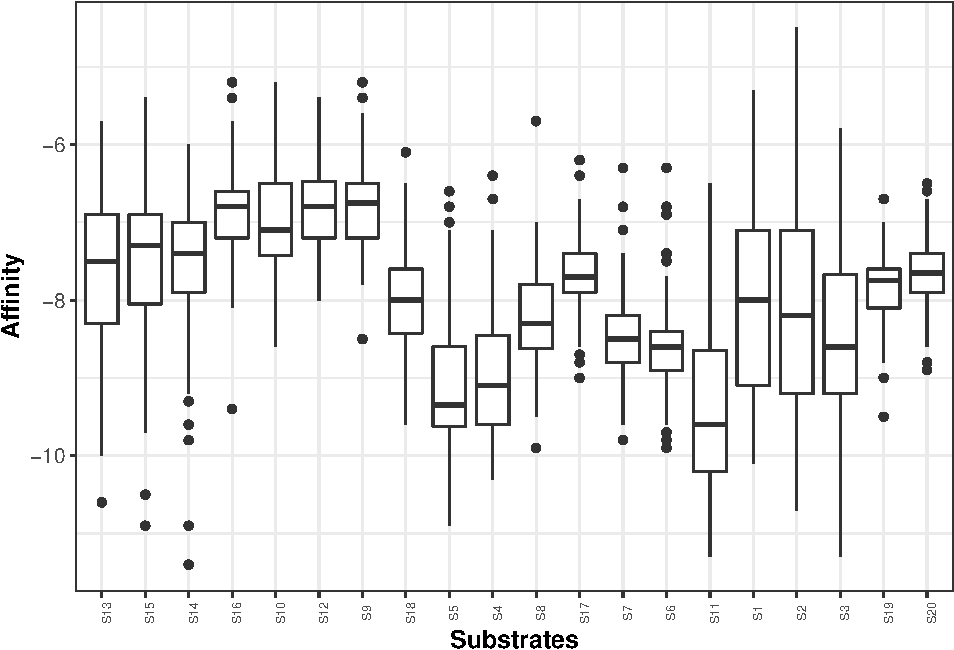
\includegraphics{tesis_files/figure-latex/substrateBox-1} \end{center}
  
  \clearpage  
  
  \section{PriA Activity on GTP}\label{pria-activity-on-gtp}
  
  Activity was measured fluorometrically in 96-well plates (Nuc 96-Well
  Optical Botto Plates) in a TECAN infinite M1000 plate reader (excitation
  at 286 nm and emission at 386 nm)
  
  Preliminar activity essays were performed on an active PriA from
  \emph{Streptomyces coelicolor} and an inactive mutant D11A.
  
  Enzymes were cloned on coli V68 strains, overexpression were induced and
  protein were purified.
  
  \begin{figure}[h!tbp]
  \centering
  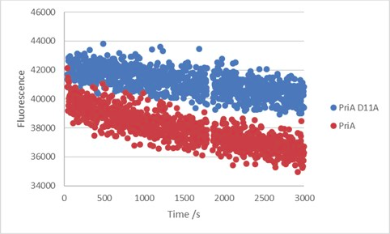
\includegraphics[angle = 0,scale = 0.6]{chapter4/MutantControl.png}
  \caption[Scoe and non functional Scoe PriA acting on dGTP]{\normalsize{Scoe and non functional Scoe PriA acting on dGTP}}
  \label{fig:PriARutas}
  \end{figure}
  
  \clearpage  
  
  \begin{Shaded}
  \begin{Highlighting}[]
  \NormalTok{GTP <-}\StringTok{ }\KeywordTok{read.table}\NormalTok{(}\StringTok{"chapter4/GTP.activity"}\NormalTok{, }\DataTypeTok{header=}\OtherTok{TRUE}\NormalTok{, }\DataTypeTok{sep=}\StringTok{"}\CharTok{\textbackslash{}t}\StringTok{"}\NormalTok{)}
  \NormalTok{dGTP <-}\StringTok{ }\KeywordTok{read.table}\NormalTok{(}\StringTok{"chapter4/dGTP.activity"}\NormalTok{, }\DataTypeTok{header=}\OtherTok{TRUE}\NormalTok{, }\DataTypeTok{sep=}\StringTok{"}\CharTok{\textbackslash{}t}\StringTok{"}\NormalTok{)}
  \NormalTok{GTP.m <-}\StringTok{ }\KeywordTok{melt}\NormalTok{(GTP,}\DataTypeTok{id=}\StringTok{"Time"}\NormalTok{)}
  
  \KeywordTok{plot}\NormalTok{(GTP.m}\OperatorTok{$}\NormalTok{Time, GTP.m}\OperatorTok{$}\NormalTok{value, }\DataTypeTok{col=}\NormalTok{GTP.m}\OperatorTok{$}\NormalTok{variable, }\DataTypeTok{pch=}\DecValTok{19}\NormalTok{)}
  \end{Highlighting}
  \end{Shaded}
  
  \begin{verbatim}
  Warning in xy.coords(x, y, xlabel, ylabel, log): NAs introducidos por
  coerción
  \end{verbatim}
  
  \begin{center}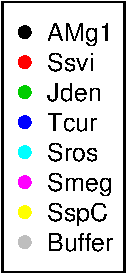
\includegraphics{tesis_files/figure-latex/activity-1} \end{center}
  
  \begin{Shaded}
  \begin{Highlighting}[]
  \KeywordTok{plot.new}\NormalTok{()}
  \KeywordTok{legend}\NormalTok{(}\StringTok{"center"}\NormalTok{, }\DataTypeTok{legend =} \KeywordTok{unique}\NormalTok{(GTP.m}\OperatorTok{$}\NormalTok{variable), }\DataTypeTok{col =} \KeywordTok{unique}\NormalTok{(GTP.m}\OperatorTok{$}\NormalTok{variable), }\DataTypeTok{pch=}\DecValTok{19}\NormalTok{)}
  \end{Highlighting}
  \end{Shaded}
  
  \begin{center}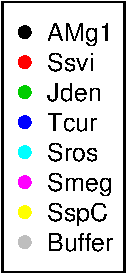
\includegraphics{tesis_files/figure-latex/activity-2} \end{center}
  
  \begin{Shaded}
  \begin{Highlighting}[]
  \KeywordTok{ggplot}\NormalTok{(GTP.m, }\KeywordTok{aes}\NormalTok{(}\DataTypeTok{x=}\NormalTok{Time, }\DataTypeTok{y=}\NormalTok{value,}\DataTypeTok{color=}\NormalTok{variable)) }\OperatorTok{+}\StringTok{ }\KeywordTok{geom_point}\NormalTok{()}\OperatorTok{+}\StringTok{ }\KeywordTok{facet_wrap}\NormalTok{(}\OperatorTok{~}\StringTok{ }\NormalTok{variable)}\OperatorTok{+}\StringTok{ }\KeywordTok{geom_smooth}\NormalTok{()}\OperatorTok{+}\KeywordTok{theme_bw}\NormalTok{()}\OperatorTok{+}\KeywordTok{theme}\NormalTok{(}\DataTypeTok{plot.title =} \KeywordTok{element_text}\NormalTok{(}\DataTypeTok{size =} \DecValTok{8}\NormalTok{, }\DataTypeTok{face =} \StringTok{"bold"}\NormalTok{), }\DataTypeTok{text =} \KeywordTok{element_text}\NormalTok{(}\DataTypeTok{size =} \DecValTok{12}\NormalTok{), }\DataTypeTok{axis.title =} \KeywordTok{element_text}\NormalTok{(}\DataTypeTok{face=}\StringTok{"bold"}\NormalTok{), }\DataTypeTok{axis.text.y=}\KeywordTok{element_text}\NormalTok{(}\DataTypeTok{angle =} \DecValTok{30}\NormalTok{,}\DataTypeTok{size =} \DecValTok{1}\NormalTok{), }\DataTypeTok{legend.position =} \StringTok{"bottom"}\NormalTok{)}\OperatorTok{+}\StringTok{ }\KeywordTok{scale_size_area}\NormalTok{()}
  \end{Highlighting}
  \end{Shaded}
  
  \begin{verbatim}
  `geom_smooth()` using method = 'loess'
  \end{verbatim}
  
  \begin{verbatim}
  Warning in simpleLoess(y, x, w, span, degree = degree, parametric =
  parametric, : span too small. fewer data values than degrees of freedom.
  \end{verbatim}
  
  \begin{verbatim}
  Warning in simpleLoess(y, x, w, span, degree = degree, parametric =
  parametric, : at 227.79
  \end{verbatim}
  
  \begin{verbatim}
  Warning in simpleLoess(y, x, w, span, degree = degree, parametric =
  parametric, : radius 64.12
  \end{verbatim}
  
  \begin{verbatim}
  Warning in simpleLoess(y, x, w, span, degree = degree, parametric =
  parametric, : all data on boundary of neighborhood. make span bigger
  \end{verbatim}
  
  \begin{verbatim}
  Warning in simpleLoess(y, x, w, span, degree = degree, parametric =
  parametric, : pseudoinverse used at 227.79
  \end{verbatim}
  
  \begin{verbatim}
  Warning in simpleLoess(y, x, w, span, degree = degree, parametric =
  parametric, : neighborhood radius 8.0075
  \end{verbatim}
  
  \begin{verbatim}
  Warning in simpleLoess(y, x, w, span, degree = degree, parametric =
  parametric, : reciprocal condition number 1
  \end{verbatim}
  
  \begin{verbatim}
  Warning in simpleLoess(y, x, w, span, degree = degree, parametric =
  parametric, : at 1845.3
  \end{verbatim}
  
  \begin{verbatim}
  Warning in simpleLoess(y, x, w, span, degree = degree, parametric =
  parametric, : radius 64.12
  \end{verbatim}
  
  \begin{verbatim}
  Warning in simpleLoess(y, x, w, span, degree = degree, parametric =
  parametric, : all data on boundary of neighborhood. make span bigger
  \end{verbatim}
  
  \begin{verbatim}
  Warning in simpleLoess(y, x, w, span, degree = degree, parametric =
  parametric, : There are other near singularities as well. 64.12
  \end{verbatim}
  
  \begin{verbatim}
  Warning in simpleLoess(y, x, w, span, degree = degree, parametric =
  parametric, : zero-width neighborhood. make span bigger
  
  Warning in simpleLoess(y, x, w, span, degree = degree, parametric =
  parametric, : zero-width neighborhood. make span bigger
  \end{verbatim}
  
  \begin{verbatim}
  Warning: Computation failed in `stat_smooth()`:
  NA/NaN/Inf en llamada a una función externa (arg 5)
  \end{verbatim}
  
  \begin{verbatim}
  Warning in simpleLoess(y, x, w, span, degree = degree, parametric =
  parametric, : span too small. fewer data values than degrees of freedom.
  \end{verbatim}
  
  \begin{verbatim}
  Warning in simpleLoess(y, x, w, span, degree = degree, parametric =
  parametric, : at 474.62
  \end{verbatim}
  
  \begin{verbatim}
  Warning in simpleLoess(y, x, w, span, degree = degree, parametric =
  parametric, : radius 15.07
  \end{verbatim}
  
  \begin{verbatim}
  Warning in simpleLoess(y, x, w, span, degree = degree, parametric =
  parametric, : all data on boundary of neighborhood. make span bigger
  \end{verbatim}
  
  \begin{verbatim}
  Warning in simpleLoess(y, x, w, span, degree = degree, parametric =
  parametric, : pseudoinverse used at 474.62
  \end{verbatim}
  
  \begin{verbatim}
  Warning in simpleLoess(y, x, w, span, degree = degree, parametric =
  parametric, : neighborhood radius 3.882
  \end{verbatim}
  
  \begin{verbatim}
  Warning in simpleLoess(y, x, w, span, degree = degree, parametric =
  parametric, : reciprocal condition number 1
  \end{verbatim}
  
  \begin{verbatim}
  Warning in simpleLoess(y, x, w, span, degree = degree, parametric =
  parametric, : at 1258.8
  \end{verbatim}
  
  \begin{verbatim}
  Warning in simpleLoess(y, x, w, span, degree = degree, parametric =
  parametric, : radius 15.07
  \end{verbatim}
  
  \begin{verbatim}
  Warning in simpleLoess(y, x, w, span, degree = degree, parametric =
  parametric, : all data on boundary of neighborhood. make span bigger
  \end{verbatim}
  
  \begin{verbatim}
  Warning in simpleLoess(y, x, w, span, degree = degree, parametric =
  parametric, : There are other near singularities as well. 15.07
  \end{verbatim}
  
  \begin{verbatim}
  Warning in simpleLoess(y, x, w, span, degree = degree, parametric =
  parametric, : zero-width neighborhood. make span bigger
  
  Warning in simpleLoess(y, x, w, span, degree = degree, parametric =
  parametric, : zero-width neighborhood. make span bigger
  \end{verbatim}
  
  \begin{verbatim}
  Warning: Computation failed in `stat_smooth()`:
  NA/NaN/Inf en llamada a una función externa (arg 5)
  \end{verbatim}
  
  \begin{verbatim}
  Warning in simpleLoess(y, x, w, span, degree = degree, parametric =
  parametric, : span too small. fewer data values than degrees of freedom.
  \end{verbatim}
  
  \begin{verbatim}
  Warning in simpleLoess(y, x, w, span, degree = degree, parametric =
  parametric, : at 859.79
  \end{verbatim}
  
  \begin{verbatim}
  Warning in simpleLoess(y, x, w, span, degree = degree, parametric =
  parametric, : radius 47.817
  \end{verbatim}
  
  \begin{verbatim}
  Warning in simpleLoess(y, x, w, span, degree = degree, parametric =
  parametric, : all data on boundary of neighborhood. make span bigger
  \end{verbatim}
  
  \begin{verbatim}
  Warning in simpleLoess(y, x, w, span, degree = degree, parametric =
  parametric, : pseudoinverse used at 859.79
  \end{verbatim}
  
  \begin{verbatim}
  Warning in simpleLoess(y, x, w, span, degree = degree, parametric =
  parametric, : neighborhood radius 6.915
  \end{verbatim}
  
  \begin{verbatim}
  Warning in simpleLoess(y, x, w, span, degree = degree, parametric =
  parametric, : reciprocal condition number 1
  \end{verbatim}
  
  \begin{verbatim}
  Warning in simpleLoess(y, x, w, span, degree = degree, parametric =
  parametric, : at 2256.6
  \end{verbatim}
  
  \begin{verbatim}
  Warning in simpleLoess(y, x, w, span, degree = degree, parametric =
  parametric, : radius 47.817
  \end{verbatim}
  
  \begin{verbatim}
  Warning in simpleLoess(y, x, w, span, degree = degree, parametric =
  parametric, : all data on boundary of neighborhood. make span bigger
  \end{verbatim}
  
  \begin{verbatim}
  Warning in simpleLoess(y, x, w, span, degree = degree, parametric =
  parametric, : There are other near singularities as well. 47.817
  \end{verbatim}
  
  \begin{verbatim}
  Warning in simpleLoess(y, x, w, span, degree = degree, parametric =
  parametric, : zero-width neighborhood. make span bigger
  
  Warning in simpleLoess(y, x, w, span, degree = degree, parametric =
  parametric, : zero-width neighborhood. make span bigger
  \end{verbatim}
  
  \begin{verbatim}
  Warning: Computation failed in `stat_smooth()`:
  NA/NaN/Inf en llamada a una función externa (arg 5)
  \end{verbatim}
  
  \begin{verbatim}
  Warning in simpleLoess(y, x, w, span, degree = degree, parametric =
  parametric, : span too small. fewer data values than degrees of freedom.
  \end{verbatim}
  
  \begin{verbatim}
  Warning in simpleLoess(y, x, w, span, degree = degree, parametric =
  parametric, : at 1084.3
  \end{verbatim}
  
  \begin{verbatim}
  Warning in simpleLoess(y, x, w, span, degree = degree, parametric =
  parametric, : radius 0.7208
  \end{verbatim}
  
  \begin{verbatim}
  Warning in simpleLoess(y, x, w, span, degree = degree, parametric =
  parametric, : all data on boundary of neighborhood. make span bigger
  \end{verbatim}
  
  \begin{verbatim}
  Warning in simpleLoess(y, x, w, span, degree = degree, parametric =
  parametric, : pseudoinverse used at 1084.3
  \end{verbatim}
  
  \begin{verbatim}
  Warning in simpleLoess(y, x, w, span, degree = degree, parametric =
  parametric, : neighborhood radius 0.849
  \end{verbatim}
  
  \begin{verbatim}
  Warning in simpleLoess(y, x, w, span, degree = degree, parametric =
  parametric, : reciprocal condition number 1
  \end{verbatim}
  
  \begin{verbatim}
  Warning in simpleLoess(y, x, w, span, degree = degree, parametric =
  parametric, : at 1255.7
  \end{verbatim}
  
  \begin{verbatim}
  Warning in simpleLoess(y, x, w, span, degree = degree, parametric =
  parametric, : radius 0.7208
  \end{verbatim}
  
  \begin{verbatim}
  Warning in simpleLoess(y, x, w, span, degree = degree, parametric =
  parametric, : all data on boundary of neighborhood. make span bigger
  \end{verbatim}
  
  \begin{verbatim}
  Warning in simpleLoess(y, x, w, span, degree = degree, parametric =
  parametric, : There are other near singularities as well. 0.7208
  \end{verbatim}
  
  \begin{verbatim}
  Warning in simpleLoess(y, x, w, span, degree = degree, parametric =
  parametric, : zero-width neighborhood. make span bigger
  
  Warning in simpleLoess(y, x, w, span, degree = degree, parametric =
  parametric, : zero-width neighborhood. make span bigger
  \end{verbatim}
  
  \begin{verbatim}
  Warning: Computation failed in `stat_smooth()`:
  NA/NaN/Inf en llamada a una función externa (arg 5)
  \end{verbatim}
  
  \begin{verbatim}
  Warning in simpleLoess(y, x, w, span, degree = degree, parametric =
  parametric, : span too small. fewer data values than degrees of freedom.
  \end{verbatim}
  
  \begin{verbatim}
  Warning in simpleLoess(y, x, w, span, degree = degree, parametric =
  parametric, : at 1470.5
  \end{verbatim}
  
  \begin{verbatim}
  Warning in simpleLoess(y, x, w, span, degree = degree, parametric =
  parametric, : radius 7.7869
  \end{verbatim}
  
  \begin{verbatim}
  Warning in simpleLoess(y, x, w, span, degree = degree, parametric =
  parametric, : all data on boundary of neighborhood. make span bigger
  \end{verbatim}
  
  \begin{verbatim}
  Warning in simpleLoess(y, x, w, span, degree = degree, parametric =
  parametric, : pseudoinverse used at 1470.5
  \end{verbatim}
  
  \begin{verbatim}
  Warning in simpleLoess(y, x, w, span, degree = degree, parametric =
  parametric, : neighborhood radius 2.7905
  \end{verbatim}
  
  \begin{verbatim}
  Warning in simpleLoess(y, x, w, span, degree = degree, parametric =
  parametric, : reciprocal condition number 1
  \end{verbatim}
  
  \begin{verbatim}
  Warning in simpleLoess(y, x, w, span, degree = degree, parametric =
  parametric, : at 2034.2
  \end{verbatim}
  
  \begin{verbatim}
  Warning in simpleLoess(y, x, w, span, degree = degree, parametric =
  parametric, : radius 7.7869
  \end{verbatim}
  
  \begin{verbatim}
  Warning in simpleLoess(y, x, w, span, degree = degree, parametric =
  parametric, : all data on boundary of neighborhood. make span bigger
  \end{verbatim}
  
  \begin{verbatim}
  Warning in simpleLoess(y, x, w, span, degree = degree, parametric =
  parametric, : There are other near singularities as well. 7.7869
  \end{verbatim}
  
  \begin{verbatim}
  Warning in simpleLoess(y, x, w, span, degree = degree, parametric =
  parametric, : zero-width neighborhood. make span bigger
  
  Warning in simpleLoess(y, x, w, span, degree = degree, parametric =
  parametric, : zero-width neighborhood. make span bigger
  \end{verbatim}
  
  \begin{verbatim}
  Warning: Computation failed in `stat_smooth()`:
  NA/NaN/Inf en llamada a una función externa (arg 5)
  \end{verbatim}
  
  \begin{verbatim}
  Warning in simpleLoess(y, x, w, span, degree = degree, parametric =
  parametric, : span too small. fewer data values than degrees of freedom.
  \end{verbatim}
  
  \begin{verbatim}
  Warning in simpleLoess(y, x, w, span, degree = degree, parametric =
  parametric, : at 2612.2
  \end{verbatim}
  
  \begin{verbatim}
  Warning in simpleLoess(y, x, w, span, degree = degree, parametric =
  parametric, : radius 2.1199
  \end{verbatim}
  
  \begin{verbatim}
  Warning in simpleLoess(y, x, w, span, degree = degree, parametric =
  parametric, : all data on boundary of neighborhood. make span bigger
  \end{verbatim}
  
  \begin{verbatim}
  Warning in simpleLoess(y, x, w, span, degree = degree, parametric =
  parametric, : pseudoinverse used at 2612.2
  \end{verbatim}
  
  \begin{verbatim}
  Warning in simpleLoess(y, x, w, span, degree = degree, parametric =
  parametric, : neighborhood radius 1.456
  \end{verbatim}
  
  \begin{verbatim}
  Warning in simpleLoess(y, x, w, span, degree = degree, parametric =
  parametric, : reciprocal condition number 1
  \end{verbatim}
  
  \begin{verbatim}
  Warning in simpleLoess(y, x, w, span, degree = degree, parametric =
  parametric, : at 2906.4
  \end{verbatim}
  
  \begin{verbatim}
  Warning in simpleLoess(y, x, w, span, degree = degree, parametric =
  parametric, : radius 2.1199
  \end{verbatim}
  
  \begin{verbatim}
  Warning in simpleLoess(y, x, w, span, degree = degree, parametric =
  parametric, : all data on boundary of neighborhood. make span bigger
  \end{verbatim}
  
  \begin{verbatim}
  Warning in simpleLoess(y, x, w, span, degree = degree, parametric =
  parametric, : There are other near singularities as well. 2.1199
  \end{verbatim}
  
  \begin{verbatim}
  Warning in simpleLoess(y, x, w, span, degree = degree, parametric =
  parametric, : zero-width neighborhood. make span bigger
  
  Warning in simpleLoess(y, x, w, span, degree = degree, parametric =
  parametric, : zero-width neighborhood. make span bigger
  \end{verbatim}
  
  \begin{verbatim}
  Warning: Computation failed in `stat_smooth()`:
  NA/NaN/Inf en llamada a una función externa (arg 5)
  \end{verbatim}
  
  \begin{center}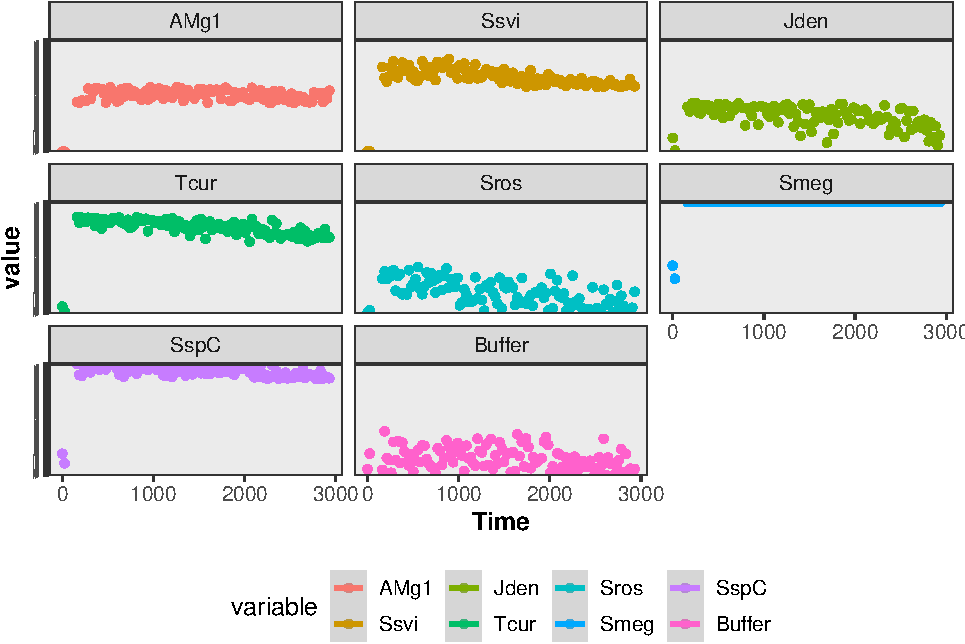
\includegraphics{tesis_files/figure-latex/activity-3} \end{center}
  
  \begin{Shaded}
  \begin{Highlighting}[]
  \KeywordTok{ggplot}\NormalTok{(GTP.m, }\KeywordTok{aes}\NormalTok{(}\DataTypeTok{x=}\NormalTok{Time, }\DataTypeTok{y=}\NormalTok{value,}\DataTypeTok{color=}\NormalTok{variable)) }\OperatorTok{+}\StringTok{ }\KeywordTok{geom_point}\NormalTok{()}\OperatorTok{+}\StringTok{ }\KeywordTok{geom_smooth}\NormalTok{()}\OperatorTok{+}\KeywordTok{theme_bw}\NormalTok{()}\OperatorTok{+}\KeywordTok{theme}\NormalTok{(}\DataTypeTok{plot.title =} \KeywordTok{element_text}\NormalTok{(}\DataTypeTok{size =} \DecValTok{8}\NormalTok{, }\DataTypeTok{face =} \StringTok{"bold"}\NormalTok{), }\DataTypeTok{text =} \KeywordTok{element_text}\NormalTok{(}\DataTypeTok{size =} \DecValTok{12}\NormalTok{), }\DataTypeTok{axis.title =} \KeywordTok{element_text}\NormalTok{(}\DataTypeTok{face=}\StringTok{"bold"}\NormalTok{), }\DataTypeTok{axis.text.y=}\KeywordTok{element_text}\NormalTok{(}\DataTypeTok{angle =} \DecValTok{30}\NormalTok{,}\DataTypeTok{size =} \DecValTok{1}\NormalTok{), }\DataTypeTok{legend.position =} \StringTok{"bottom"}\NormalTok{)}\OperatorTok{+}\StringTok{ }\KeywordTok{scale_size_area}\NormalTok{()}
  \end{Highlighting}
  \end{Shaded}
  
  \begin{verbatim}
  `geom_smooth()` using method = 'loess'
  \end{verbatim}
  
  \begin{verbatim}
  Warning in simpleLoess(y, x, w, span, degree = degree, parametric =
  parametric, : span too small. fewer data values than degrees of freedom.
  \end{verbatim}
  
  \begin{verbatim}
  Warning in simpleLoess(y, x, w, span, degree = degree, parametric =
  parametric, : at 1470.5
  \end{verbatim}
  
  \begin{verbatim}
  Warning in simpleLoess(y, x, w, span, degree = degree, parametric =
  parametric, : radius 7.7869
  \end{verbatim}
  
  \begin{verbatim}
  Warning in simpleLoess(y, x, w, span, degree = degree, parametric =
  parametric, : all data on boundary of neighborhood. make span bigger
  \end{verbatim}
  
  \begin{verbatim}
  Warning in simpleLoess(y, x, w, span, degree = degree, parametric =
  parametric, : pseudoinverse used at 1470.5
  \end{verbatim}
  
  \begin{verbatim}
  Warning in simpleLoess(y, x, w, span, degree = degree, parametric =
  parametric, : neighborhood radius 2.7905
  \end{verbatim}
  
  \begin{verbatim}
  Warning in simpleLoess(y, x, w, span, degree = degree, parametric =
  parametric, : reciprocal condition number 1
  \end{verbatim}
  
  \begin{verbatim}
  Warning in simpleLoess(y, x, w, span, degree = degree, parametric =
  parametric, : at 2034.2
  \end{verbatim}
  
  \begin{verbatim}
  Warning in simpleLoess(y, x, w, span, degree = degree, parametric =
  parametric, : radius 7.7869
  \end{verbatim}
  
  \begin{verbatim}
  Warning in simpleLoess(y, x, w, span, degree = degree, parametric =
  parametric, : all data on boundary of neighborhood. make span bigger
  \end{verbatim}
  
  \begin{verbatim}
  Warning in simpleLoess(y, x, w, span, degree = degree, parametric =
  parametric, : There are other near singularities as well. 7.7869
  \end{verbatim}
  
  \begin{verbatim}
  Warning in simpleLoess(y, x, w, span, degree = degree, parametric =
  parametric, : zero-width neighborhood. make span bigger
  
  Warning in simpleLoess(y, x, w, span, degree = degree, parametric =
  parametric, : zero-width neighborhood. make span bigger
  \end{verbatim}
  
  \begin{verbatim}
  Warning: Computation failed in `stat_smooth()`:
  NA/NaN/Inf en llamada a una función externa (arg 5)
  \end{verbatim}
  
  \begin{center}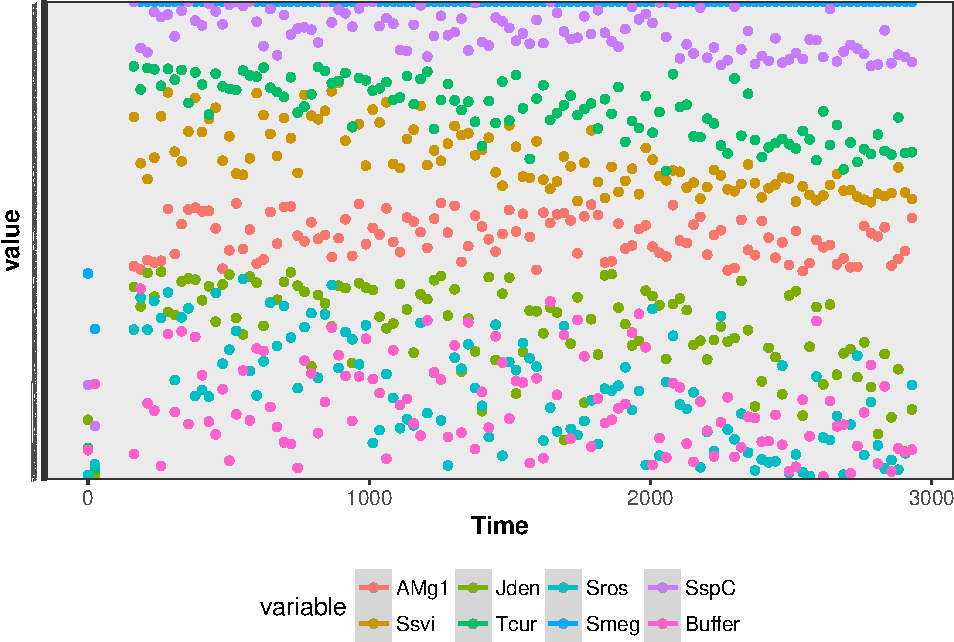
\includegraphics{tesis_files/figure-latex/activity-4} \end{center}
  
  the two enzymes with activity\\
  \emph{Thermomonospora curvata} thermophilic Actinobacteria from
  Thermomonosporaceae genus, it can be found in compost and participate in
  the active degradation of cellulose
  {[}\protect\hyperlink{ref-chertkov_complete_2011}{137}{]}.
  
  Jonesia trpF shows no activity \emph{Jonesia denitrificans} is
  classified as a pathogenic organism for animals, reported genome was
  originally isolated from cooked ox blood
  {[}\protect\hyperlink{ref-pukall_complete_2009}{138}{]}.
  
  \begin{Shaded}
  \begin{Highlighting}[]
  \NormalTok{docking <-}\StringTok{ }\KeywordTok{read.csv}\NormalTok{(}\StringTok{"chapter4/SmallHeat.data"}\NormalTok{, }\DataTypeTok{header=}\OtherTok{TRUE}\NormalTok{, }\DataTypeTok{sep=}\StringTok{"}\CharTok{\textbackslash{}t}\StringTok{"}\NormalTok{)}
  \KeywordTok{kable}\NormalTok{(docking,  }\DataTypeTok{caption =} \StringTok{"Enzymes docking }\CharTok{\textbackslash{}\textbackslash{}}\StringTok{label\{tab:docking\}"}\NormalTok{,}\DataTypeTok{caption.short =} \StringTok{"Enzymes docking "}\NormalTok{)}
  \end{Highlighting}
  \end{Shaded}
  
  \begin{longtable}[]{@{}lrrrrrrrrrrrrrrrrrrrr@{}}
  \caption{Enzymes docking \label{tab:docking}}\tabularnewline
  \toprule
  Enzima & S13 & S15 & S14 & S16 & S10 & S12 & S9 & S18 & S5 & S4 & S8 &
  S17 & S7 & S6 & S11 & S1 & S2 & S3 & S19 & S20\tabularnewline
  \midrule
  \endfirsthead
  \toprule
  Enzima & S13 & S15 & S14 & S16 & S10 & S12 & S9 & S18 & S5 & S4 & S8 &
  S17 & S7 & S6 & S11 & S1 & S2 & S3 & S19 & S20\tabularnewline
  \midrule
  \endhead
  Srub\_2VEP & -7.4 & -7.3 & -7.5 & -7.1 & -6.5 & -6.2 & -6.5 & -7.7 &
  -9.4 & -9.3 & -7.9 & -7.2 & -8.3 & -8.6 & -8.9 & -9.0 & -7.1 & -8.9 &
  -7.8 & -7.7\tabularnewline
  Saver\_2VEP & -7.4 & -7.2 & -7.0 & -6.5 & -7.3 & -6.4 & -7.0 & -7.5 &
  -9.6 & -8.5 & -7.9 & -7.6 & -8.4 & -8.7 & -9.8 & -8.3 & -7.9 & -8.6 &
  -7.7 & -7.6\tabularnewline
  Scoe\_2VEP & -7.5 & -7.5 & -7.9 & -7.0 & -7.0 & -6.2 & -6.5 & -7.8 &
  -8.8 & -9.2 & -7.8 & -7.9 & -8.0 & -8.9 & -10.3 & -9.2 & -9.3 & -8.4 &
  -8.1 & -8.2\tabularnewline
  Scoe\_2X30 & -8.1 & -7.4 & -7.6 & -6.9 & -6.7 & -6.8 & -7.1 & -7.9 &
  -9.1 & -9.0 & -8.3 & -8.6 & -8.5 & -9.0 & -10.6 & -10.0 & -10.3 & -10.2
  & -8.1 & -7.9\tabularnewline
  Scoe\_1VZW & NA & NA & NA & NA & NA & NA & NA & NA & NA & NA & NA & NA &
  NA & NA & NA & NA & NA & NA & NA & NA\tabularnewline
  Sfla\_2VEP & -7.1 & -7.6 & -7.2 & -7.3 & -7.2 & -6.8 & -6.9 & -8.1 &
  -8.2 & -7.2 & -8.2 & -7.2 & -8.4 & -8.3 & -8.5 & -7.9 & -7.8 & -6.0 &
  -7.5 & -7.3\tabularnewline
  Sgha\_2VEP & -9.2 & -8.7 & -6.7 & -6.7 & -7.4 & -7.7 & -7.2 & -7.5 &
  -9.8 & -8.9 & -8.2 & -7.8 & -8.8 & -8.7 & -10.1 & -9.1 & -9.0 & -9.5 &
  -8.0 & -7.5\tabularnewline
  Siak\_2VEP & -6.6 & -7.3 & -7.0 & -7.1 & -7.1 & -7.1 & -6.8 & -8.0 &
  -9.2 & -8.7 & -7.8 & -7.6 & -8.3 & -8.4 & -9.1 & -5.8 & -5.3 & -8.5 &
  -7.3 & -7.4\tabularnewline
  Sbic\_2VEP & -7.2 & -6.7 & -6.8 & -6.5 & -6.2 & -6.6 & -5.9 & -7.8 &
  -8.5 & -7.8 & -7.8 & -7.2 & -8.2 & -8.0 & -9.6 & -8.2 & -8.0 & -9.4 &
  -7.7 & -7.5\tabularnewline
  Sbot\_2VEP & -9.6 & -10.9 & -8.9 & -7.1 & -6.0 & -6.2 & -6.7 & -8.1 &
  -9.1 & -8.8 & -8.3 & -7.9 & -8.9 & -9.3 & -9.4 & -9.8 & -10.0 & -8.9 &
  -8.2 & -8.0\tabularnewline
  Sipo\_2VEP & -6.6 & -6.6 & -7.3 & -6.9 & -6.5 & -6.3 & -6.5 & -8.1 &
  -8.6 & -9.1 & -8.0 & -7.9 & -8.0 & -8.4 & -8.5 & -7.2 & -8.4 & -8.2 &
  -7.9 & -7.6\tabularnewline
  Ssvi & NA & NA & NA & NA & NA & NA & NA & NA & NA & NA & NA & NA & NA &
  NA & NA & NA & NA & NA & NA & NA\tabularnewline
  Ssvi\_4U28 & NA & NA & NA & NA & NA & NA & NA & NA & NA & NA & NA & NA &
  NA & NA & NA & NA & NA & NA & NA & NA\tabularnewline
  Ssvi\_4TX9 & -5.9 & -8.2 & -7.1 & -6.6 & -6.8 & -7.0 & -7.6 & -7.9 &
  -8.4 & -8.3 & -8.2 & -8.1 & -8.4 & -8.7 & -7.7 & -8.2 & -8.2 & -6.7 &
  -8.0 & -7.5\tabularnewline
  Salb\_2VEP & -6.3 & -7.1 & -7.4 & -6.8 & -7.7 & -6.9 & -6.6 & -8.0 &
  -9.6 & -8.9 & -8.6 & -7.9 & -8.6 & -8.4 & -9.1 & -7.4 & -7.2 & -8.8 &
  -8.1 & -7.8\tabularnewline
  Sbik\_2VEP & -7.4 & -6.7 & -7.4 & -7.3 & -7.7 & -6.5 & -6.8 & -8.5 &
  -9.9 & -9.8 & -8.3 & -7.8 & -8.2 & -8.4 & -10.5 & -7.1 & -6.3 & -8.3 &
  -8.1 & -7.9\tabularnewline
  Stsu\_2VEP & -6.9 & -7.5 & -7.9 & -7.8 & -7.5 & -7.3 & -7.7 & -8.1 &
  -10.0 & -9.7 & -8.7 & -7.8 & -8.8 & -8.8 & -10.6 & -7.8 & -8.7 & -9.2 &
  -7.9 & -7.8\tabularnewline
  Sven\_2VEP & -8.3 & -7.6 & -7.5 & -6.8 & -6.4 & -7.0 & -6.2 & -8.2 &
  -9.6 & -9.0 & -7.9 & -7.4 & -8.3 & -8.6 & -10.0 & -8.2 & -8.2 & -8.1 &
  -7.6 & -7.4\tabularnewline
  Scal\_2VEP & -7.3 & -8.8 & -7.5 & -6.7 & -7.0 & -6.5 & -6.5 & -8.7 &
  -10.0 & -9.7 & -8.8 & -7.7 & -8.2 & -8.6 & -10.5 & -8.1 & -9.2 & -8.9 &
  -7.6 & -7.6\tabularnewline
  Sbaa\_2VEP & -8.9 & -6.6 & -6.7 & -6.8 & -7.2 & -7.2 & -6.2 & -7.7 &
  -9.6 & -9.5 & -8.4 & -7.4 & -8.5 & -8.2 & -9.7 & -8.5 & -8.4 & -9.3 &
  -7.4 & -7.7\tabularnewline
  Sglo\_2VEP & -6.1 & -6.8 & -6.9 & -6.5 & -6.7 & -6.3 & -6.7 & -7.5 &
  -9.6 & -9.6 & -8.6 & -7.8 & -8.7 & -8.7 & -9.9 & -6.2 & -5.1 & -9.2 &
  -7.8 & -7.7\tabularnewline
  Sful\_2VEP & -9.0 & -6.9 & -7.1 & -6.8 & -6.3 & -7.2 & -6.6 & -8.1 &
  -9.8 & -9.3 & -7.7 & -8.0 & -8.7 & -8.8 & -10.5 & -7.6 & -9.1 & -10.5 &
  -7.1 & -7.4\tabularnewline
  Sgri\_2VEP & -6.6 & -8.2 & -7.1 & -6.4 & -7.1 & -7.4 & -7.1 & -7.4 &
  -9.4 & -8.5 & -8.6 & -7.5 & -8.8 & -8.4 & -9.6 & -8.8 & -8.8 & -8.7 &
  -7.7 & -7.5\tabularnewline
  S34\_2VEP & -7.8 & -7.2 & -7.6 & -7.3 & -6.2 & -6.5 & -6.9 & -8.0 & -8.8
  & -8.6 & -7.7 & -7.1 & -7.7 & -7.9 & -7.2 & -7.1 & -6.7 & -7.1 & -7.7 &
  -7.7\tabularnewline
  Srim\_2VEP & -7.4 & -6.8 & -7.1 & -7.2 & -7.2 & -7.4 & -7.8 & -8.6 &
  -9.7 & -9.3 & -8.8 & -7.7 & -8.9 & -8.7 & -10.2 & -6.8 & -8.2 & -9.0 &
  -7.5 & -7.8\tabularnewline
  Satr\_2VEP & -7.6 & -7.1 & -7.5 & -7.4 & -6.2 & -6.5 & -6.9 & -8.0 &
  -8.9 & -8.7 & -7.7 & -7.4 & -7.7 & -7.8 & -6.5 & -7.0 & -6.3 & -7.7 &
  -7.7 & -7.7\tabularnewline
  S1813\_2VEP & -7.5 & -6.7 & -6.8 & -6.6 & -6.8 & -7.0 & -6.7 & -7.9 &
  -9.9 & -9.7 & -8.3 & -7.7 & -8.5 & -8.6 & -10.0 & -7.6 & -7.5 & -8.6 &
  -7.3 & -7.5\tabularnewline
  Svar\_2VEP & -6.3 & -6.8 & -7.0 & -6.3 & -6.9 & -6.9 & -6.6 & -7.8 &
  -9.3 & -7.4 & -8.5 & -7.3 & -8.0 & -8.7 & -8.5 & -7.4 & -6.3 & -6.0 &
  -7.9 & -7.5\tabularnewline
  Sfra\_2VEP & -7.3 & -7.0 & -6.8 & -6.6 & -6.5 & -7.3 & -6.6 & -8.6 &
  -9.1 & -8.7 & -8.9 & -7.7 & -8.9 & -9.0 & -8.7 & -6.0 & -6.3 & -7.9 &
  -8.2 & -7.8\tabularnewline
  Smeg\_2VEP & -8.0 & -7.3 & -6.9 & -6.6 & -7.2 & -6.7 & -6.1 & -7.6 &
  -9.2 & -9.1 & -7.8 & -7.4 & -8.2 & -8.5 & -9.6 & -9.2 & -9.2 & -8.6 &
  -7.7 & -7.5\tabularnewline
  Ssul\_2VEP & -7.5 & -7.0 & -6.9 & -6.6 & -6.6 & -6.7 & -6.9 & -7.7 &
  -8.4 & -8.2 & -8.2 & -7.5 & -8.1 & -7.7 & -8.2 & -6.7 & -7.1 & -7.7 &
  -7.6 & -7.4\tabularnewline
  Slav\_4X9S & -8.0 & -7.1 & -6.7 & -6.9 & -6.6 & -6.8 & -6.7 & -8.2 &
  -9.5 & -9.1 & -8.6 & -8.0 & -8.4 & -8.7 & -9.1 & -9.5 & -9.3 & -8.1 &
  -8.1 & -7.6\tabularnewline
  Sery\_4X9S & -7.8 & -7.2 & -7.6 & -7.2 & -7.4 & -6.9 & -7.4 & -8.5 &
  -9.4 & -9.4 & -8.6 & -7.6 & -8.4 & -8.6 & -9.1 & -10.0 & -10.1 & -9.0 &
  -7.8 & -8.2\tabularnewline
  SspC\_4X9S & -7.4 & -6.9 & -7.3 & -6.8 & -7.3 & -6.6 & -7.5 & -8.0 &
  -9.8 & -9.3 & -8.7 & -7.6 & -8.5 & -8.4 & -10.6 & -9.1 & -8.9 & -8.5 &
  -8.1 & -8.0\tabularnewline
  Sxan\_4X9S & -7.5 & -6.9 & -6.8 & -6.8 & -6.5 & -6.6 & -6.5 & -8.3 &
  -8.0 & -8.1 & -7.6 & -7.4 & -8.7 & -8.1 & -8.1 & -8.5 & -8.0 & -7.6 &
  -7.7 & -7.4\tabularnewline
  Skat\_4X9S & -6.4 & -7.0 & -7.1 & -6.7 & -7.7 & -6.3 & -6.2 & -8.1 &
  -8.5 & -9.2 & -8.3 & -7.6 & -9.0 & -8.5 & -9.7 & -9.5 & -9.9 & -9.2 &
  -7.4 & -7.5\tabularnewline
  SMg1\_4X9S & -6.5 & -6.9 & -7.2 & -7.1 & -6.5 & -6.9 & -6.4 & -7.3 &
  -7.8 & -7.7 & -8.3 & -7.5 & -7.9 & -8.4 & -9.5 & -7.6 & -5.2 & -7.5 &
  -7.6 & -7.7\tabularnewline
  SMg1\_W9T & NA & NA & NA & NA & NA & NA & NA & NA & NA & NA & NA & NA &
  NA & NA & NA & NA & NA & NA & NA & NA\tabularnewline
  Sniv\_2VEP & -6.2 & -6.8 & -7.4 & -6.5 & -7.8 & -6.8 & -6.7 & -9.5 &
  -9.6 & -9.4 & -8.7 & -8.2 & -8.6 & -9.1 & -9.9 & -5.4 & -5.5 & -9.2 &
  -8.0 & -7.5\tabularnewline
  Scla\_2VEP & -6.4 & -7.7 & -7.4 & -7.2 & -7.6 & -7.5 & -7.2 & -8.5 &
  -10.1 & -10.0 & -8.7 & -7.9 & -8.8 & -9.1 & -10.2 & -6.9 & -8.1 & -8.5 &
  -7.7 & -7.7\tabularnewline
  Save\_2VEP & -7.6 & -6.7 & -7.1 & -7.2 & -7.1 & -6.5 & -6.6 & -7.8 &
  -8.6 & -10.0 & -8.6 & -7.5 & -8.3 & -8.5 & -8.8 & -5.3 & -5.2 & -5.8 &
  -7.7 & -7.4\tabularnewline
  Spur\_2vEP & -6.8 & -7.3 & -6.9 & -6.7 & -8.0 & -7.9 & -7.7 & -8.5 &
  -9.5 & -9.8 & -8.1 & -7.8 & -8.7 & -9.7 & -10.0 & -5.3 & -6.2 & -8.2 &
  -7.6 & -7.4\tabularnewline
  Scar\_2Y89 & -6.9 & -6.8 & -7.5 & -7.1 & -7.8 & -7.3 & -7.2 & -8.3 &
  -9.2 & -8.3 & -8.9 & -8.4 & -8.9 & -9.3 & -9.4 & -5.3 & -5.2 & -7.1 &
  -8.5 & -8.6\tabularnewline
  Mtub\_2Y88 & -10.0 & -7.8 & -8.9 & -5.4 & -8.6 & -7.3 & -7.8 & -9.5 &
  -10.9 & -10.3 & -9.5 & -9.0 & -9.8 & -9.8 & -11.3 & -10.1 & -10.2 &
  -11.3 & -9.5 & -8.8\tabularnewline
  Mtub\_2Y89 & -8.7 & -8.6 & -9.6 & -9.4 & -6.4 & -5.9 & -5.6 & -7.1 &
  -7.0 & -7.5 & -7.3 & -6.8 & -7.4 & -8.4 & -7.5 & -8.1 & -8.6 & -7.5 &
  -7.7 & -7.3\tabularnewline
  Mtub\_2Y85 & -8.2 & -7.9 & -9.2 & -7.4 & -7.6 & -7.5 & -7.6 & -8.4 &
  -9.7 & -9.5 & -9.3 & -7.8 & -8.6 & -8.6 & -10.2 & -9.8 & -9.9 & -10.1 &
  -7.3 & -7.4\tabularnewline
  Mtub\_3ZS4 & -10.0 & -10.5 & -11.4 & -6.4 & -8.2 & -7.2 & -7.0 & -9.6 &
  -10.2 & -10.2 & -9.9 & -8.5 & -9.3 & -9.6 & -10.9 & -10.0 & -10.7 & -9.9
  & -8.8 & -8.9\tabularnewline
  S34\_3ZS4 & -7.4 & -8.0 & -7.6 & -6.4 & -5.2 & -5.4 & -5.2 & -6.1 & -6.8
  & -6.4 & -5.7 & -6.4 & -6.3 & -6.3 & -7.1 & -7.4 & -7.1 & -6.4 & -7.1 &
  -6.6\tabularnewline
  Cdip\_4AXK & -9.2 & -7.8 & -10.9 & -7.2 & -7.5 & -7.6 & -7.7 & -8.9 &
  -9.0 & -9.8 & -9.0 & -8.3 & -8.8 & -9.2 & -10.1 & -9.5 & -9.9 & -9.2 &
  -8.0 & -7.9\tabularnewline
  Cjei\_4AXK & -7.5 & -6.9 & -7.2 & -6.5 & -8.4 & -8.0 & -8.5 & -8.7 &
  -9.5 & -9.6 & -9.4 & -8.8 & -9.0 & -9.5 & -9.3 & -8.1 & -9.3 & -8.5 &
  -7.9 & -7.7\tabularnewline
  Aaur & NA & NA & NA & NA & NA & NA & NA & NA & NA & NA & NA & NA & NA &
  NA & NA & NA & NA & NA & NA & NA\tabularnewline
  Aaur\_4WD0 & -8.2 & -8.5 & -8.1 & -7.9 & -5.7 & -5.5 & -5.9 & -7.0 &
  -7.5 & -7.2 & -7.1 & -6.7 & -7.1 & -7.4 & -8.4 & -7.2 & -7.3 & -7.4 &
  -7.0 & -6.7\tabularnewline
  Acar\_4X2R & -10.6 & -9.3 & -9.3 & -7.2 & -7.2 & -6.8 & -7.3 & -7.5 &
  -9.5 & -9.8 & -8.0 & -7.8 & -9.3 & -8.9 & -10.3 & -9.6 & -9.4 & -9.4 &
  -8.1 & -8.0\tabularnewline
  Auro\_4X2R & -9.9 & -9.1 & -9.8 & -8.1 & -7.4 & -7.1 & -7.4 & -7.8 &
  -9.2 & -9.8 & -8.3 & -7.8 & -9.3 & -9.0 & -9.9 & -9.0 & -8.6 & -9.2 &
  -8.5 & -8.2\tabularnewline
  Afer\_4WD0 & -5.7 & -5.8 & -6.0 & -5.7 & -6.7 & -6.2 & -5.8 & -7.6 &
  -9.2 & -8.8 & -7.8 & -7.4 & -8.3 & -8.4 & -9.3 & -6.7 & -4.5 & -9.1 &
  -8.3 & -8.1\tabularnewline
  Sent\_5AHE & -9.1 & -5.4 & -6.4 & -5.2 & -8.0 & -7.3 & -7.4 & -8.8 &
  -10.7 & -10.2 & -8.7 & -8.7 & -9.6 & -9.9 & -10.9 & -7.8 & -9.1 & -10.3
  & -9.0 & -8.4\tabularnewline
  Ecoli\_K12 & -9.7 & -9.7 & -9.2 & -6.1 & -7.2 & -6.6 & -6.8 & -8.6 &
  -9.5 & -9.1 & -8.6 & -8.2 & -9.0 & -8.6 & -10.2 & -9.9 & -10.2 & -9.9 &
  -8.2 & -7.9\tabularnewline
  Jden\_4WUI & -8.3 & -8.8 & -8.2 & -6.8 & -6.2 & -6.1 & -6.0 & -6.8 &
  -7.4 & -7.6 & -7.5 & -6.9 & -7.6 & -7.5 & -7.7 & -7.5 & -7.6 & -7.2 &
  -7.3 & -7.2\tabularnewline
  Ctra & -8.2 & -8.0 & -7.4 & -7.2 & -6.1 & -5.5 & -5.4 & -6.5 & -7.1 &
  -7.1 & -7.0 & -6.2 & -6.8 & -6.8 & -6.9 & -7.2 & -7.4 & -6.5 & -6.7 &
  -6.6\tabularnewline
  SMg1\_trpF & -7.2 & -8.8 & -8.2 & -7.3 & -6.2 & -5.7 & -5.7 & -6.9 &
  -6.6 & -6.7 & -7.3 & -6.7 & -7.6 & -6.9 & -7.5 & -7.1 & -7.1 & -6.9 &
  -6.7 & -6.5\tabularnewline
  Aodo\_4X2R & -8.5 & -8.6 & -8.8 & -7.3 & -7.1 & -7.1 & -7.1 & -7.5 &
  -9.7 & -9.4 & -7.8 & -7.6 & -9.6 & -8.8 & -10.1 & -8.4 & -8.9 & -9.4 &
  -8.0 & -8.1\tabularnewline
  \clearpage & & & & & & & & & & & & & & & & & & & &\tabularnewline
  \bottomrule
  \end{longtable}
  
  \section{Molecular dynamics vs experimental
  data}\label{molecular-dynamics-vs-experimental-data}
  
  PriA activity on S3 (PRA)
  
  \[ 
  \begin{tabular}{ l c r l l l l l}
  \hline \\ [-1.5ex]
  organism  &Family & $K_M    $     & $k_{cat}$        & $\frac{k_{cat}}{K_M}$ &Pre MD & Pos MD & Reference  \\ [1ex]
  \hline \\ [-1.5ex]
  Afer        &HisA   & $1.1\pm0.2$   &$  0.05\pm0.001    $& 0.045                  &-10.1    &-12.3       &Noda-García L et al 2015\\ [1ex]
  Ecoli       &HisA   &$  1.6         $&$         4.9       $&3.1                   &-9.9   &-16       &Henn-Sax et al. (2002)\\ [1ex]
  Sent        &HisA   &$  17.0 \pm0.1 $&$ 7.8 \pm 2.4   $&$4.5 × 10^5          $&-10.3  &-20.1     &Söderholm A et al (2015)\\ [1ex]
  Aaur        &PriB   &$  2.1 \pm 0.5 $& $    1.8 \pm 0.2     $&0.9                   &-7.4   &              &verduzco-castro 2016\\ [1ex]
  Sipo        &PriB   &$  3.8\pm0.2     $&$0.82\pm0.02        $&0.21                  &-8.2     &-14.7       &verduzco-castro 2016\\ [1ex]
  SspC        &PriB   &$  11.4\pm3.4  $&$2.53\pm0.74      $&0.22                  &   -8.5    &-12.7     &verduzco-castro 2016\\ [1ex]
  SMg1        &PriB   &$  13.2\pm3.4  $&$0.92\pm0.19      $&0.069                 &-8     &-15.2     &verduzco-castro 2016\\ [1ex]
  Ssvi        &PriB   &$  3.9\pm0.89  $&$0.69\pm0.04      $&0.18                  &-8.2     &-16.7     &verduzco-castro 2016\\ [1ex]
  Scoe        &PriA   &$  3.6\pm0.7     $&$ 1.3\pm0.2     $  &0.4                   &-8.4   &-15       &Noda-García et al (2010)\\ [1ex]
  Sglob       &PriA   & $4.2\pm0.8     $ & $0.74\pm0.03    $   &0.18                  &-9.2     &-16.7       &verduzco-castro\\ [1ex]
  Mtub 2Y85   &priA   &$  19  0.23      $&$0.012  -9.7          $&                      &       &          &Due et al 2011\\ [1ex]
  Mtub 3ZS4   &priA   &$  ?                 $&$-9.9               $&                      &       &          &Due et al 2011 (To be published)\\ [1ex]
  Auro        &priA   &$  4.0 \pm 0.9 $&$0.2 \pm 0.03   $&0.04                    &-9.2       &          &Vazquez-Juarez (2016)\\ [1ex]
  Cjei        &PriA   &$  2.3 \pm 0.2 $&$0.9 \pm 0.08   $&0.39                    &-8.5       &          &Noda-García et al (2013)\\ [1ex]
  Cdip        &subHisA&$  4.4 \pm 0.5 $&$2.6 \pm 0.3      $&0.59                  &-9.2       &          &Noda-García et al (2013)\\ [1ex]
  SMg1 TrpF   &TrpF3  &   -                &-                &-                       &-6.9     &-9.6      &verduzco-castro 2016\\ [1ex]
  Jden        &TrpF3  &   -                &-                &-          -7.2         &-9.4     &$16.8\pm3.3$&    Verduzco-Castro E et al  2016\\ [1ex]
  Acar      &SubHisA& 0.02                     &                 &                        &       &          &            \\ [1ex]
  Aodo        &SubTrpF&       -              &-                  &-                     &       &          &\\ [1ex]
  \hline
  \end{tabular}
  \label{table:name}
  \]
  
  PriA activity on S7 (PROFAR) \$\$ \centering 
  
  \begin{tabular}{ l c r l l l l l}
  \hline \\ [-1.5ex]
  organism  &Family  &  $K_M$ & $k_{cat}$& $\frac{k{cat}}{K_M}$ &Pre MD &Pos MD &Reference  \\ [1ex]
  \hline \\ [-1.5ex]
  Afer      &HisA    &-            &-                &-          &-9.2    &-9        &Noda-García L et al. (2015)   \\ [1ex]
  Ecoli     &HisA    &-            &-                &-          &-9      &-11.1     &Henn-Sax et al. (2002)\\ [1ex]
  Sent      &HisA    &-            & -               &-          &-9.6    &-10.2     &Söderholm A et al (2015)\\ [1ex]
  Aaur      &PriB    &$26.3\pm6.3$ & $0.37\pm 0.09$  & 0.014     &-7.1    &-         &verduzco-castro 2016\\ [1ex]
  Sipo      &PriB    &$60.8\pm1.1$ &$8.25\pm0.4 $    &0.14       &-8      &-8.5      &verduzco-castro 2016 \\ [1ex]
  SspC      &PriB    &$149.9\pm29$ &$1.4\pm0.12 $    &0.009      &-8.5    &-10.8     &verduzco-castro 2016\\ [1ex]
  SMg1      &PriB    &$129.6\pm34$ &$0.29\pm0.04$    &0.0022     &-7.5    &-11       &verduzco-castro 2016\\ [1ex]
  Ssvi      &PriB    &$24.5\pm4.0$ &$1.6\pm0.29 $    &0.067      &-8      &-9.7      &verduzco-castro 2016 \\ [1ex]
  Scoe      &PriA    &$5.0\pm0.08$ &$3.4\pm0.09  $   &0.7        &-8      &-9.4      &Noda-García et al (2010)   \\ [1ex]
  Sglob     &PriA    &$11\pm1.0$  &$3.8\pm0.2  $     &0.34       &-8.7    &-9.4      &verduzco-castro 2016  \\ [1ex]
  Mtub2Y85  &priA    &21         &3.6         &0.17       &-8.6    &          &Due et al 2011                        \\ [1ex] 
  Mtub3ZS4  &priA    &           &            &           &-9.3    &          &Due et al 2011 (To be published)      \\ [1ex] 
  Auro      &priA    &$23 \pm 6.5 $  &$0.5\pm0.05 $&0.02       &-9.3    &          &Vazquez-Juarez (2016)                 \\ [1ex] 
  Cjei      &PriA    &$5.1 \pm1.0$  &$1.6 \pm 0.16 $&0.31       &-9      &          &Noda-García et al (2013)              \\ [1ex]
  Cdip      &subHisA &-          &-           &-          &-8.8    &          &Noda-García et al (2013)              \\ [1ex]
  SMg1 TrpF &TrpF3   &$8.4\pm1.7$    &$10.5\pm2.4$    &1.25       &-7.6    &-9        &verduzco-castro     \\ [1ex] 
  Jden      &TrpF3   &$16.8\pm3.3$   &$27\pm1.6$      &1.6        &-7.6    &-7.7      &verduzco-castro     \\ [1ex] 
  Acar      &SubHisA &Na         &Na          &0.02       &Na      &Na        &Na                                    \\ [1ex] 
  Aodo      &SubTrpF &-          &-           &-          &-       &Na        &Na                                    \\ [1ex]
  
  \hline
  \end{tabular}
  
  \label{table:mi table}\$\$
  
  Con actividad de FolE i.e activa para el compuesto V Adams et al (2014)
  Genome size vs Total antismash cluster coloured by order
  
  \clearpage  
  
  \section{Non darwinian trayectories}\label{non-darwinian-trayectories}
  
  \begin{figure}[h!tbp]
  \centering
  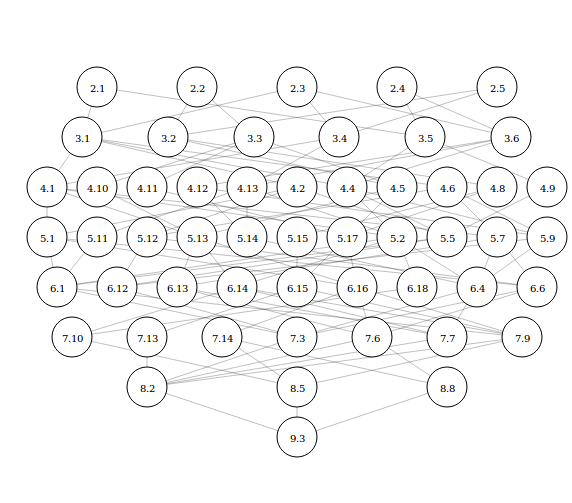
\includegraphics[angle = 0,scale = 0.6]{conclusion/Solocirculos.png}
  \caption[Non darwinian trayectories]{\normalsize{Non darwinian trayectories}}
  \label{fig:PriARutas}
  \end{figure}
  
  \begin{figure}[h!tbp]
  \centering
  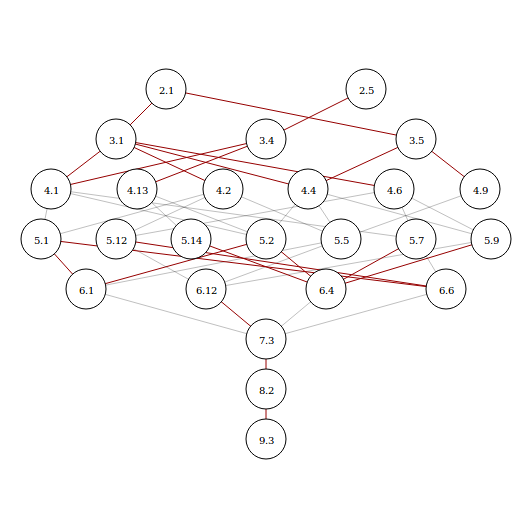
\includegraphics[angle = 0,scale = 0.6]{conclusion/SolocirculosPRA.png}
  \caption[Positive increments on PRA]{\normalsize{Positive increments on PRA}}
  \label{fig:PRARutas}
  \end{figure}
  
  \begin{figure}[h!tbp]
  \centering
  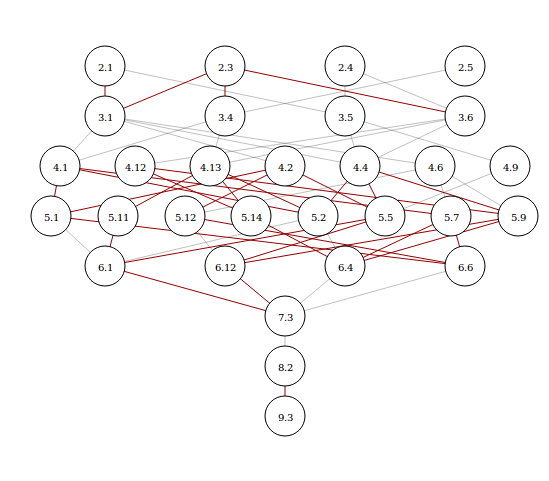
\includegraphics[angle = 0,scale = 0.6]{conclusion/SolocirculosPRO.png}
  \caption[Positive increments on ProFAR]{\normalsize{Positive increments on ProFAR}}
  \label{fig:ProFARRutas}
  \end{figure}
  
  HisF Arabinosa TrpC TrpD acido antranilico PRPP gliceroles de Ana checar
  resistencias
  
  \begin{figure}[h!tbp]
  \centering
  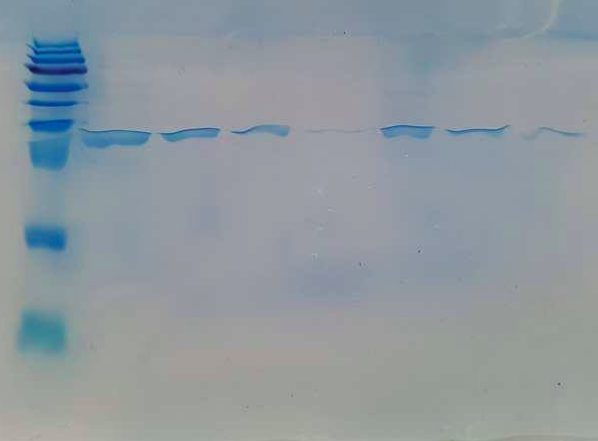
\includegraphics[angle = 0,scale = 0.6]{chapter4/Geles/PriAAbril30.png}
  \caption[gel]{\normalsize{gel}}
  \label{fig:gel}
  \end{figure}
  
  \begin{Shaded}
  \begin{Highlighting}[]
  \CommentTok{#sessionInfo()}
  \end{Highlighting}
  \end{Shaded}
  
  \chapter*{Conclusion}\label{conclusion}
  \addcontentsline{toc}{chapter}{Conclusion}
  
  \setcounter{chapter}{4} \setcounter{section}{0}
  
  Idea de Rosario -ver dell cluster de saxitoxin cuantos pasos se
  necesitron para llegar ahi.\\
  -A donde se iria el resultado de abrir el GMP\\
  -Otra vez, que Actinos tienen FolE
  
  If we don't want Conclusion to have a chapter number next to it, we can
  add the \texttt{\{.unnumbered\}} attribute. This has an unintended
  consequence of the sections being labeled as 3.6 for example though
  instead of 4.1. The \LaTeX~commands immediately following the Conclusion
  declaration get things back on track.
  
  \subsubsection{More info}\label{more-info}
  
  And here's some other random info: the first paragraph after a chapter
  title or section head \emph{shouldn't be} indented, because indents are
  to tell the reader that you're starting a new paragraph. Since that's
  obvious after a chapter or section title, proper typesetting doesn't add
  an indent there.
  
  \appendix
  
  \chapter{The First Appendix}\label{the-first-appendix}
  
  This first appendix includes all of the R chunks of code that were
  hidden throughout the document (using the \texttt{include\ =\ FALSE}
  chunk tag) to help with readibility and/or setup.
  
  \subsubsection{In the main Rmd file:}\label{in-the-main-rmd-file}
  
  \begin{Shaded}
  \begin{Highlighting}[]
  \CommentTok{# This chunk ensures that the reedtemplates package is}
  \CommentTok{# installed and loaded. This reedtemplates package includes}
  \CommentTok{# the template files for the thesis and also two functions}
  \CommentTok{# used for labeling and referencing}
  \ControlFlowTok{if}\NormalTok{(}\OperatorTok{!}\KeywordTok{require}\NormalTok{(devtools))}
    \KeywordTok{install.packages}\NormalTok{(}\StringTok{"devtools"}\NormalTok{, }\DataTypeTok{repos =} \StringTok{"http://cran.rstudio.com"}\NormalTok{)}
  \ControlFlowTok{if}\NormalTok{(}\OperatorTok{!}\KeywordTok{require}\NormalTok{(reedtemplates))\{}
    \KeywordTok{library}\NormalTok{(devtools)}
  \NormalTok{  devtools}\OperatorTok{::}\KeywordTok{install_github}\NormalTok{(}\StringTok{"ismayc/reedtemplates"}\NormalTok{)}
  \NormalTok{\}}
  \KeywordTok{library}\NormalTok{(reedtemplates)}
  \end{Highlighting}
  \end{Shaded}
  
  \subsubsection{\texorpdfstring{In
  \protect\hyperlink{ref_labels}{}:}{In :}}\label{in}
  
  \chapter{The Second Appendix, Open source code on this
  document}\label{the-second-appendix-open-source-code-on-this-document}
  
  \section{R markdown}\label{r-markdown}
  
  Thanks to Rmakdown Thesis\\
  Apendix one Useful docker commands\\
  -Create a new repository\\
  \texttt{docker\ build\ .\ -t\ evomining}\\
  \texttt{docker\ push\ nselemevomining}
  
  \section{Docker}\label{docker}
  
  Restart docker and free all ports\\
  \texttt{sudo\ service\ docker\ restart}
  
  list containers\\
  \texttt{docker\ ps\ -a}
  
  ssh or bash into a running docker container\\
  \texttt{sudo\ docker\ exec\ -i\ -t\ romantic\_brahmagupta\ /bin/bash}
  \texttt{docker\ exec\ -it\ \textless{}mycontainer\textgreater{}\ bash}
  
  Stop all containers\\
  \texttt{docker\ rm\ \$(docker\ ps\ -a\ -q)}
  
  Remove stopped containers\\
  \texttt{docker\ rm\ \$(docker\ ps\ -q\ -f\ status=exited)}
  
  Remove all images\\
  \texttt{docker\ rmi\ \$(docker\ images\ -q)}
  
  uninstall docker from ubuntu (Fresh start)\\
  \texttt{sudo\ apt-get\ purge\ docker-engine}\\
  \texttt{sudo\ apt-get\ autoremove\ -\/-purge\ docker-engine}\\
  \texttt{rm\ -rf\ /var/lib/docker} \# This deletes all images,
  containers, and volumes
  
  Run Evomining container using nselem/newevomining image\\
  \texttt{docker\ run\ -i\ -t\ -v\ /home/nelly/GIT/EvoMining/:/var/www/html/EvoMining/exchange\ -p\ 80:80\ nselem/newevomining\ /bin/bash}
  
  Start evomining inside this container\\
  \texttt{perl\ startevomining}
  
  Vizualice a tree\\
  \texttt{http://10.10.100.234/EvoMining/cgi-bin/color\_tree.pl?9\&\&/var/www/html/EvoMining/exchange/CyanosBBH\_MiBIG\_DB.faa\_CYANOS}
  file 9.new must be on folder volume CyanosBBH\_MiBIG\_DB.faa\_CYANOS
  
  Find a perl module\\
  \texttt{perl\ -MList::Util\ -e\textquotesingle{}print\ \$\_\ .\ "\ =\textgreater{}\ "\ .\ \$INC\{\$\_\}\ .\ "\textbackslash{}n"\ for\ keys\ \%INC\textquotesingle{}}
  EvoMining notes\\
  Gblocks only runs inside folder /var/www/html/EvoMining
  
  \section{Git}\label{git}
  
  \texttt{git\ add\ -\/-all}\\
  \texttt{git\ commit\ -m\ "Some\ message"}\\
  \texttt{git\ push\ -u\ origin\ master}\\
  \texttt{git\ clone}
  
  \section{Connect GitHub and
  DockerHub}\label{connect-github-and-dockerhub}
  
  automated builds The Dockerfile is available to anyone with access to
  your Docker Hub repository. Your repository is kept up-to-date with code
  changes automatically.
  
  \section{Additional resources}\label{additional-resources}
  
  \begin{itemize}
  \item
    \emph{Markdown} Cheatsheet -
    \url{https://github.com/adam-p/markdown-here/wiki/Markdown-Cheatsheet}
  \item
    \emph{R Markdown} Reference Guide -
    \url{https://www.rstudio.com/wp-content/uploads/2015/03/rmarkdown-reference.pdf}
  \item
    Introduction to \texttt{dplyr} -
    \url{https://cran.rstudio.com/web/packages/dplyr/vignettes/introduction.html}
  \item
    \texttt{ggplot2} Documentation -
    \url{http://docs.ggplot2.org/current/}
  \end{itemize}
  
  Docker antiSMASH run\_antismash /.gbk \textasciitilde{}/as\_results
  --knownclusterblast --inclusive --cf\_threshold 0.7
  
  \chapter{The third Appendix, Other contributions during my
  phd}\label{the-third-appendix-other-contributions-during-my-phd}
  
  \section{Accepted}\label{accepted}
  
  -Evomining identifies Arsenolipids biosynthetic cluster
  
  \section{Submitted}\label{submitted}
  
  \begin{itemize}
  \tightlist
  \item
    Siderophore micrococcus cluster identified by CORASON\\
  \item
    CORASON find genomes that owns cluster from cyanobacterial
    metagenome\\
  \item
    Streptomyces central pathways expanssions
  \end{itemize}
  
  \section{On preparation}\label{on-preparation}
  
  \begin{itemize}
  \tightlist
  \item
    PriA non Darwinian trayectories\\
    poner figura James unidades docking
  \end{itemize}
  
  \backmatter
  
  \chapter{References}\label{references}
  
  \noindent
  
  \setlength{\parindent}{-0.20in} \setlength{\leftskip}{0.20in}
  \setlength{\parskip}{8pt}
  
  \hypertarget{refs}{}
  \hypertarget{ref-cruz-morales_phylogenomic_2016}{}
  1. Cruz-Morales P, Kopp JF, Martínez-Guerrero C, Yáñez-Guerra LA,
  Selem-Mojica N, Ramos-Aboites H, et al. Phylogenomic Analysis of Natural
  Products Biosynthetic Gene Clusters Allows Discovery of Arseno-Organic
  Metabolites in Model Streptomycetes. Genome Biology and Evolution
  {[}Internet{]}. 2016 Jun {[}cited 2017 Jan 24{]};8(6):1906--16.
  Available from: \url{http://gbe.oxfordjournals.org/content/8/6/1906}
  
  \hypertarget{ref-koonin_turbulent_2015}{}
  2. Koonin EV. The Turbulent Network Dynamics of Microbial Evolution and
  the Statistical Tree of Life. Journal of Molecular Evolution
  {[}Internet{]}. 2015 {[}cited 2017 Jan 28{]};80(5-6):244--50. Available
  from: \url{http://www.ncbi.nlm.nih.gov/pmc/articles/PMC4472940/}
  
  \hypertarget{ref-halachev_calculating_2011}{}
  3. Halachev MR, Loman NJ, Pallen MJ. Calculating Orthologs in Bacteria
  and Archaea: A Divide and Conquer Approach. PLOS ONE {[}Internet{]}.
  2011 Dec {[}cited 2016 Sep 16{]};6(12):e28388. Available from:
  \url{http://journals.plos.org/plosone/article?id=10.1371/journal.pone.0028388}
  
  \hypertarget{ref-narechania_random_2012}{}
  4. Narechania A, Baker RH, Sit R, Kolokotronis S-O, DeSalle R, Planet
  PJ. Random Addition Concatenation Analysis: A Novel Approach to the
  Exploration of Phylogenomic Signal Reveals Strong Agreement between Core
  and Shell Genomic Partitions in the Cyanobacteria. Genome Biology and
  Evolution {[}Internet{]}. 2012 Jan {[}cited 2017 Jan 23{]};4(1):30--43.
  Available from: \url{http://gbe.oxfordjournals.org/content/4/1/30}
  
  \hypertarget{ref-aziz_rast_2008}{}
  5. Aziz RK, Bartels D, Best AA, DeJongh M, Disz T, Edwards RA, et al.
  The RAST Server: Rapid Annotations using Subsystems Technology. BMC
  Genomics {[}Internet{]}. 2008 Feb {[}cited 2017 Feb 7{]};9:75. Available
  from: \url{http://www.ncbi.nlm.nih.gov/pmc/articles/PMC2265698/}
  
  \hypertarget{ref-overbeek_seed_2014}{}
  6. Overbeek R, Olson R, Pusch GD, Olsen GJ, Davis JJ, Disz T, et al. The
  SEED and the Rapid Annotation of microbial genomes using Subsystems
  Technology (RAST). Nucleic Acids Research {[}Internet{]}. 2014 Jan
  {[}cited 2017 Feb 7{]};42(Database issue):D206--14. Available from:
  \url{http://www.ncbi.nlm.nih.gov/pmc/articles/PMC3965101/}
  
  \hypertarget{ref-brettin_rasttk:_2015}{}
  7. Brettin T, Davis JJ, Disz T, Edwards RA, Gerdes S, Olsen GJ, et al.
  RASTtk: A modular and extensible implementation of the RAST algorithm
  for building custom annotation pipelines and annotating batches of
  genomes. Scientific Reports {[}Internet{]}. 2015 Feb {[}cited 2017 Feb
  7{]};5:8365. Available from:
  \url{http://www.nature.com/srep/2015/150210/srep08365/full/srep08365.html}
  
  \hypertarget{ref-chesterismay_updated_2016}{}
  8. chesterismay. Updated R Markdown thesis template {[}Internet{]}.
  Chester's R blog. 2016 {[}cited 2017 Feb 7{]}. Available from:
  \url{https://chesterismay.wordpress.com/2016/09/01/updated-r-markdown-thesis-template/}
  
  \hypertarget{ref-barona-gomez_what_2012}{}
  9. Barona-Gómez F, Cruz-Morales P, Noda-García L. What can genome-scale
  metabolic network reconstructions do for prokaryotic systematics?
  Antonie van Leeuwenhoek {[}Internet{]}. 2012 Jan {[}cited 2017 Jan
  24{]};101(1):35--43. Available from:
  \url{http://link.springer.com/article/10.1007/s10482-011-9655-1}
  
  \hypertarget{ref-weber_antismash_2015}{}
  10. Weber T, Blin K, Duddela S, Krug D, Kim HU, Bruccoleri R, et al.
  antiSMASH 3.0---a comprehensive resource for the genome mining of
  biosynthetic gene clusters. Nucleic Acids Research {[}Internet{]}. 2015
  Jul {[}cited 2017 Feb 7{]};43(W1):W237--43. Available from:
  \url{https://academic.oup.com/nar/article/43/W1/W237/2467910/antiSMASH-3-0-a-comprehensive-resource-for-the}
  
  \hypertarget{ref-medema_antismash:_2011}{}
  11. Medema MH, Blin K, Cimermancic P, Jager V de, Zakrzewski P,
  Fischbach MA, et al. antiSMASH: Rapid identification, annotation and
  analysis of secondary metabolite biosynthesis gene clusters in bacterial
  and fungal genome sequences. Nucleic Acids Research {[}Internet{]}. 2011
  Jul {[}cited 2017 Feb 7{]};39(Web Server issue):W339--46. Available
  from: \url{http://www.ncbi.nlm.nih.gov/pmc/articles/PMC3125804/}
  
  \hypertarget{ref-khersonsky_enzyme_2010}{}
  12. Khersonsky O, Tawfik DS. Enzyme promiscuity: A mechanistic and
  evolutionary perspective. Annual Review of Biochemistry.
  2010;79:471--505.
  
  \hypertarget{ref-copley_enzymes_2003}{}
  13. Copley SD. Enzymes with extra talents: Moonlighting functions and
  catalytic promiscuity. Current Opinion in Chemical Biology
  {[}Internet{]}. 2003 Apr {[}cited 2017 Feb 8{]};7(2):265--72. Available
  from:
  \url{https://www.sciencedirect.com/science/article/pii/S1367593103000322}
  
  \hypertarget{ref-hult_enzyme_2007}{}
  14. Hult K, Berglund P. Enzyme promiscuity: Mechanism and applications.
  Trends in Biotechnology {[}Internet{]}. 2007 May {[}cited 2017 Feb
  8{]};25(5):231--8. Available from:
  \url{https://www.sciencedirect.com/science/article/pii/S016777990700073X}
  
  \hypertarget{ref-obrien_catalytic_1999}{}
  15. O'Brien PJ, Herschlag D. Catalytic promiscuity and the evolution of
  new enzymatic activities. Chemistry \& Biology {[}Internet{]}. 1999 Apr
  {[}cited 2017 Feb 9{]};6(4):R91--R105. Available from:
  \url{http://www.sciencedirect.com/science/article/pii/S1074552199800337}
  
  \hypertarget{ref-baronagomez_occurrence_2003}{}
  16. Barona Gómez F, Hodgson DA. Occurrence of a putative ancient like
  isomerase involved in histidine and tryptophan biosynthesis. EMBO
  reports {[}Internet{]}. 2003 Mar {[}cited 2017 Feb 8{]};4(3):296--300.
  Available from: \url{http://embor.embopress.org/content/4/3/296}
  
  \hypertarget{ref-risso_phenotypic_2014}{}
  17. Risso VA, Gavira JA, Gaucher EA, Sanchez Ruiz JM. Phenotypic
  comparisons of consensus variants versus laboratory resurrections of
  precambrian proteins. Proteins: Structure, Function, and Bioinformatics
  {[}Internet{]}. 2014 Jun {[}cited 2017 Feb 9{]};82(6):887--96. Available
  from:
  \url{http://onlinelibrary.wiley.com/doi/10.1002/prot.24575/abstract}
  
  \hypertarget{ref-kumari_preparation_2007}{}
  18. Kumari V, Shah S, Gupta MN. Preparation of Biodiesel by
  Lipase-Catalyzed Transesterification of High Free Fatty Acid Containing
  Oil from Madhuca indica. Energy \& Fuels {[}Internet{]}. 2007 Jan
  {[}cited 2017 Feb 8{]};21(1):368--72. Available from:
  \url{http://dx.doi.org/10.1021/ef0602168}
  
  \hypertarget{ref-li_computational_2004}{}
  19. Li C, Henry CS, Jankowski MD, Ionita JA, Hatzimanikatis V, Broadbelt
  LJ. Computational discovery of biochemical routes to specialty
  chemicals. Chemical Engineering Science {[}Internet{]}. 2004 Nov
  {[}cited 2017 Feb 8{]};59(22--23):5051--60. Available from:
  \url{https://www.sciencedirect.com/science/article/pii/S0009250904006669}
  
  \hypertarget{ref-glasner_evolution_2006}{}
  20. Glasner ME, Gerlt JA, Babbitt PC. Evolution of enzyme superfamilies.
  Current Opinion in Chemical Biology {[}Internet{]}. 2006 Oct {[}cited
  2017 Feb 9{]};10(5):492--7. Available from:
  \url{https://www.sciencedirect.com/science/article/pii/S1367593106001177}
  
  \hypertarget{ref-baier_evolution_2016}{}
  21. Baier F, Copp JN, Tokuriki N. Evolution of Enzyme Superfamilies:
  Comprehensive Exploration of Sequence--Function Relationships.
  Biochemistry {[}Internet{]}. 2016 Nov {[}cited 2017 Feb
  8{]};55(46):6375--88. Available from:
  \url{http://dx.doi.org/10.1021/acs.biochem.6b00723}
  
  \hypertarget{ref-bloom_neutral_2007}{}
  22. Bloom JD, Romero PA, Lu Z, Arnold FH. Neutral genetic drift can
  alter promiscuous protein functions, potentially aiding functional
  evolution. Biology Direct {[}Internet{]}. 2007 {[}cited 2017 Feb
  8{]};2:17. Available from:
  \url{http://dx.doi.org/10.1186/1745-6150-2-17}
  
  \hypertarget{ref-nath_quantitative_2008}{}
  23. Nath A, Atkins WM. A Quantitative Index of Substrate Promiscuity.
  Biochemistry {[}Internet{]}. 2008 Jan {[}cited 2017 Feb
  9{]};47(1):157--66. Available from:
  \url{http://dx.doi.org/10.1021/bi701448p}
  
  \hypertarget{ref-zou_evolution_2015}{}
  24. Zou T, Risso VA, Gavira JA, Sanchez-Ruiz JM, Ozkan SB. Evolution of
  Conformational Dynamics Determines the Conversion of a Promiscuous
  Generalist into a Specialist Enzyme. Molecular Biology and Evolution
  {[}Internet{]}. 2015 Jan {[}cited 2017 Feb 9{]};32(1):132--43. Available
  from:
  \url{https://academic.oup.com/mbe/article/32/1/132/2925568/Evolution-of-Conformational-Dynamics-Determines}
  
  \hypertarget{ref-firn_darwinian_2009}{}
  25. Firn RD, Jones CG. A Darwinian view of metabolism: Molecular
  properties determine fitness. Journal of Experimental Botany
  {[}Internet{]}. 2009 Mar {[}cited 2017 Feb 8{]};60(3):719--26. Available
  from:
  \url{https://academic.oup.com/jxb/article/60/3/719/452667/A-Darwinian-view-of-metabolism-molecular}
  
  \hypertarget{ref-jia_multifunctional_2013}{}
  26. Jia B, Cheong G-W, Zhang S. Multifunctional enzymes in archaea:
  Promiscuity and moonlight. Extremophiles {[}Internet{]}. 2013 Mar
  {[}cited 2017 Feb 8{]};17(2):193--203. Available from:
  \url{http://link.springer.com/article/10.1007/s00792-012-0509-1}
  
  \hypertarget{ref-aharoni_evolvability_2005}{}
  27. Aharoni A, Gaidukov L, Khersonsky O, Gould SM, Roodveldt C, Tawfik
  DS. The 'evolvability' of promiscuous protein functions. Nature Genetics
  {[}Internet{]}. 2005 Jan {[}cited 2017 Feb 8{]};37(1):73--6. Available
  from: \url{http://www.nature.com/ng/journal/v37/n1/full/ng1482.html}
  
  \hypertarget{ref-jensen_enzyme_1976}{}
  28. Jensen. Enzyme Recruitment in Evolution of New Function. Annual
  Review of Microbiology {[}Internet{]}. 1976 {[}cited 2017 Feb
  8{]};30(1):409--25. Available from:
  \url{http://dx.doi.org/10.1146/annurev.mi.30.100176.002205}
  
  \hypertarget{ref-pandya_enzyme_2014}{}
  29. Pandya C, Farelli JD, Dunaway-Mariano D, Allen KN. Enzyme
  Promiscuity: Engine of Evolutionary Innovation. Journal of Biological
  Chemistry {[}Internet{]}. 2014 Oct {[}cited 2017 Feb
  9{]};289(44):30229--36. Available from:
  \url{http://www.jbc.org/content/289/44/30229}
  
  \hypertarget{ref-dean_mechanistic_2007}{}
  30. Dean AM, Thornton JW. Mechanistic approaches to the study of
  evolution. Nature reviews Genetics {[}Internet{]}. 2007 Sep {[}cited
  2017 Feb 8{]};8(9):675--88. Available from:
  \url{http://www.ncbi.nlm.nih.gov/pmc/articles/PMC2488205/}
  
  \hypertarget{ref-nobeli_protein_2009}{}
  31. Nobeli I, Favia AD, Thornton JM. Protein promiscuity and its
  implications for biotechnology. Nature Biotechnology {[}Internet{]}.
  2009 Feb {[}cited 2017 Feb 9{]};27(2):157--67. Available from:
  \url{http://www.nature.com/nbt/journal/v27/n2/full/nbt1519.html}
  
  \hypertarget{ref-hopkins_drug_2009}{}
  32. Hopkins AL. Drug discovery: Predicting promiscuity. Nature
  {[}Internet{]}. 2009 Nov {[}cited 2017 Feb 8{]};462(7270):167--8.
  Available from:
  \url{http://www.nature.com/nature/journal/v462/n7270/full/462167a.html}
  
  \hypertarget{ref-nath_quantifying_2010}{}
  33. Nath A, Zientek MA, Burke BJ, Jiang Y, Atkins WM. Quantifying and
  Predicting the Promiscuity and Isoform Specificity of Small-Molecule
  Cytochrome P450 Inhibitors. Drug Metabolism and Disposition
  {[}Internet{]}. 2010 Dec {[}cited 2017 Feb 9{]};38(12):2195--203.
  Available from: \url{http://dmd.aspetjournals.org/content/38/12/2195}
  
  \hypertarget{ref-von_eichborn_promiscuous:_2011}{}
  34. Eichborn J von, Murgueitio MS, Dunkel M, Koerner S, Bourne PE,
  Preissner R. PROMISCUOUS: A database for network-based
  drug-repositioning. Nucleic Acids Research {[}Internet{]}. 2011 Jan
  {[}cited 2017 Feb 9{]};39(suppl\_1):D1060--6. Available from:
  \url{https://academic.oup.com/nar/article/39/suppl_1/D1060/2506056/PROMISCUOUS-a-database-for-network-based-drug}
  
  \hypertarget{ref-zhang_multidimensional_2012}{}
  35. Zhang W, Dourado DFAR, Fernandes PA, Ramos MJ, Mannervik B.
  Multidimensional epistasis and fitness landscapes in enzyme evolution.
  Biochemical Journal {[}Internet{]}. 2012 Jul {[}cited 2017 Feb
  9{]};445(1):39--46. Available from:
  \url{http://www.biochemj.org/content/445/1/39}
  
  \hypertarget{ref-sanchez-ruiz_promiscuity_2012}{}
  36. Sanchez-Ruiz JM. On promiscuity, changing environments and the
  possibility of replaying the molecular tape of life. Biochemical Journal
  {[}Internet{]}. 2012 Jul {[}cited 2017 Feb 9{]};445(1):e1--3. Available
  from: \url{http://www.biochemj.org/content/445/1/e1}
  
  \hypertarget{ref-martinez-nunez_lifestyle_2015}{}
  37. Martínez-Núñez MA, Rodríguez-Vázquez K, Pérez-Rueda E. The lifestyle
  of prokaryotic organisms influences the repertoire of promiscuous
  enzymes. Proteins: Structure, Function, and Bioinformatics
  {[}Internet{]}. 2015 Sep {[}cited 2017 Feb 8{]};83(9):1625--31.
  Available from:
  \url{http://onlinelibrary.wiley.com/doi/10.1002/prot.24847/abstract}
  
  \hypertarget{ref-patrick_multicopy_2007}{}
  38. Patrick WM, Quandt EM, Swartzlander DB, Matsumura I. Multicopy
  Suppression Underpins Metabolic Evolvability. Molecular Biology and
  Evolution {[}Internet{]}. 2007 Dec {[}cited 2017 Feb
  9{]};24(12):2716--22. Available from:
  \url{https://academic.oup.com/mbe/article/24/12/2716/978039/Multicopy-Suppression-Underpins-Metabolic}
  
  \hypertarget{ref-notebaart_network-level_2014}{}
  39. Notebaart RA, Szappanos B, Kintses B, Pál F, Györkei Á, Bogos B, et
  al. Network-level architecture and the evolutionary potential of
  underground metabolism. Proceedings of the National Academy of Sciences
  {[}Internet{]}. 2014 Aug {[}cited 2017 Feb 9{]};111(32):11762--7.
  Available from: \url{http://www.pnas.org/content/111/32/11762}
  
  \hypertarget{ref-linster_metabolite_2013}{}
  40. Linster CL, Van Schaftingen E, Hanson AD. Metabolite damage and its
  repair or pre-emption. Nature Chemical Biology {[}Internet{]}. 2013 Feb
  {[}cited 2017 Feb 8{]};9(2):72--80. Available from:
  \url{http://www.nature.com/nchembio/journal/v9/n2/full/nchembio.1141.html}
  
  \hypertarget{ref-khanal_differential_2015}{}
  41. Khanal A, Yu McLoughlin S, Kershner JP, Copley SD. Differential
  Effects of a Mutation on the Normal and Promiscuous Activities of
  Orthologs: Implications for Natural and Directed Evolution. Molecular
  Biology and Evolution {[}Internet{]}. 2015 Jan {[}cited 2017 Feb
  8{]};32(1):100--8. Available from:
  \url{https://academic.oup.com/mbe/article/32/1/100/2925554/Differential-Effects-of-a-Mutation-on-the-Normal}
  
  \hypertarget{ref-ma_unconventional_2013}{}
  42. Ma H-M, Zhou Q, Tang Y-M, Zhang Z, Chen Y-S, He H-Y, et al.
  Unconventional Origin and Hybrid System for Construction of
  Pyrrolopyrrole Moiety in Kosinostatin Biosynthesis. Chemistry \& Biology
  {[}Internet{]}. 2013 Jun {[}cited 2017 Feb 8{]};20(6):796--805.
  Available from:
  \url{https://www.sciencedirect.com/science/article/pii/S1074552113001701}
  
  \hypertarget{ref-adams_promiscuous_2014}{}
  43. Adams NE, Thiaville JJ, Proestos J, Juárez-Vázquez AL, McCoy AJ,
  Barona-Gómez F, et al. Promiscuous and Adaptable Enzymes Fill ``Holes''
  in the Tetrahydrofolate Pathway in Chlamydia Species. mBio
  {[}Internet{]}. 2014 Jul {[}cited 2017 Jan 31{]};5(4). Available from:
  \url{http://www.ncbi.nlm.nih.gov/pmc/articles/PMC4161248/}
  
  \hypertarget{ref-soskine_mutational_2010}{}
  44. Soskine M, Tawfik DS. Mutational effects and the evolution of new
  protein functions. Nature Reviews Genetics {[}Internet{]}. 2010 Aug
  {[}cited 2017 Feb 9{]};11(8):572--82. Available from:
  \url{http://www.nature.com/nrg/journal/v11/n8/full/nrg2808.html}
  
  \hypertarget{ref-kislyuk_genomic_2011}{}
  45. Kislyuk AO, Haegeman B, Bergman NH, Weitz JS. Genomic fluidity: An
  integrative view of gene diversity within microbial populations. BMC
  Genomics {[}Internet{]}. 2011 {[}cited 2017 Jan 26{]};12:32. Available
  from: \url{http://dx.doi.org/10.1186/1471-2164-12-32}
  
  \hypertarget{ref-pearson_prehistoric_2012}{}
  46. Pearson H. Prehistoric proteins: Raising the dead. Nature News
  {[}Internet{]}. 2012 Mar {[}cited 2017 Feb 9{]};483(7390):390. Available
  from:
  \url{http://www.nature.com/news/prehistoric-proteins-raising-the-dead-1.10261}
  
  \hypertarget{ref-hughes_evolution_1994}{}
  47. Hughes AL. The Evolution of Functionally Novel Proteins after Gene
  Duplication. Proceedings of the Royal Society of London B: Biological
  Sciences {[}Internet{]}. 1994 May {[}cited 2017 Feb
  8{]};256(1346):119--24. Available from:
  \url{http://rspb.royalsocietypublishing.org/content/256/1346/119}
  
  \hypertarget{ref-treangen_horizontal_2011}{}
  48. Treangen TJ, Rocha EPC. Horizontal Transfer, Not Duplication, Drives
  the Expansion of Protein Families in Prokaryotes. PLOS Genetics
  {[}Internet{]}. 2011 Jan {[}cited 2017 Feb 9{]};7(1):e1001284. Available
  from:
  \url{http://journals.plos.org/plosgenetics/article?id=10.1371/journal.pgen.1001284}
  
  \hypertarget{ref-overbeek_use_1999}{}
  49. Overbeek R, Fonstein M, D'Souza M, Pusch GD, Maltsev N. The use of
  gene clusters to infer functional coupling. Proceedings of the National
  Academy of Sciences {[}Internet{]}. 1999 Mar {[}cited 2017 Feb
  9{]};96(6):2896--901. Available from:
  \url{http://www.pnas.org/content/96/6/2896}
  
  \hypertarget{ref-zhao_prediction_2014}{}
  50. Zhao S, Sakai A, Zhang X, Vetting MW, Kumar R, Hillerich B, et al.
  Prediction and characterization of enzymatic activities guided by
  sequence similarity and genome neighborhood networks. eLife
  {[}Internet{]}. 2014 Jun {[}cited 2017 Feb 9{]};3:e03275. Available
  from: \url{https://elifesciences.org/content/3/e03275v2}
  
  \hypertarget{ref-zhao_discovery_2013}{}
  51. Zhao S, Kumar R, Sakai A, Vetting MW, Wood BM, Brown S, et al.
  Discovery of new enzymes and metabolic pathways by using structure and
  genome context. Nature {[}Internet{]}. 2013 Oct {[}cited 2017 Feb
  9{]};502(7473):698--702. Available from:
  \url{http://www.nature.com/nature/journal/v502/n7473/full/nature12576.html}
  
  \hypertarget{ref-verdel-aranda_molecular_2015}{}
  52. Verdel-Aranda K, López-Cortina ST, Hodgson DA, Barona-Gómez F.
  Molecular annotation of ketol-acid reductoisomerases from Streptomyces
  reveals a novel amino acid biosynthesis interlock mediated by enzyme
  promiscuity. Microbial Biotechnology {[}Internet{]}. 2015 Mar {[}cited
  2017 Feb 9{]};8(2):239--52. Available from:
  \url{http://onlinelibrary.wiley.com/doi/10.1111/1751-7915.12175/abstract}
  
  \hypertarget{ref-szklarczyk_string_2015}{}
  53. Szklarczyk D, Franceschini A, Wyder S, Forslund K, Heller D,
  Huerta-Cepas J, et al. STRING v10: Protein--protein interaction
  networks, integrated over the tree of life. Nucleic Acids Research
  {[}Internet{]}. 2015 Jan {[}cited 2017 Feb 9{]};43(D1):D447--52.
  Available from:
  \url{https://academic.oup.com/nar/article/43/D1/D447/2435295/STRING-v10-protein-protein-interaction-networks}
  
  \hypertarget{ref-snel_string:_2000}{}
  54. Snel B, Lehmann G, Bork P, Huynen MA. STRING: A web-server to
  retrieve and display the repeatedly occurring neighbourhood of a gene.
  Nucleic Acids Research {[}Internet{]}. 2000 Sep {[}cited 2017 Feb
  9{]};28(18):3442--4. Available from:
  \url{http://www.ncbi.nlm.nih.gov/pmc/articles/PMC110752/}
  
  \hypertarget{ref-medema_computational_2015}{}
  55. Medema MH, Fischbach MA. Computational approaches to natural product
  discovery. Nature Chemical Biology {[}Internet{]}. 2015 Sep {[}cited
  2017 Jan 24{]};11(9):639--48. Available from:
  \url{http://www.nature.com/nchembio/journal/v11/n9/full/nchembio.1884.html}
  
  \hypertarget{ref-noda-garcia_evolution_2013}{}
  56. Noda-García L, Camacho-Zarco AR, Medina-Ruíz S, Gaytán P,
  Carrillo-Tripp M, Fülöp V, et al. Evolution of Substrate Specificity in
  a Recipient's Enzyme Following Horizontal Gene Transfer. Molecular
  Biology and Evolution {[}Internet{]}. 2013 Sep {[}cited 2017 Jan
  31{]};30(9):2024--34. Available from:
  \url{https://academic.oup.com/mbe/article/30/9/2024/1000280/Evolution-of-Substrate-Specificity-in-a-Recipient}
  
  \hypertarget{ref-carbonell_molecular_2010}{}
  57. Carbonell P, Faulon J-L. Molecular signatures-based prediction of
  enzyme promiscuity. Bioinformatics {[}Internet{]}. 2010 Aug {[}cited
  2017 Feb 8{]};26(16):2012--9. Available from:
  \url{https://academic.oup.com/bioinformatics/article/26/16/2012/215921/Molecular-signatures-based-prediction-of-enzyme}
  
  \hypertarget{ref-cheng_global_2012}{}
  58. Cheng X-Y, Huang W-J, Hu S-C, Zhang H-L, Wang H, Zhang J-X, et al. A
  Global Characterization and Identification of Multifunctional Enzymes.
  PLoS ONE {[}Internet{]}. 2012 Jun {[}cited 2017 Feb 8{]};7(6). Available
  from: \url{http://www.ncbi.nlm.nih.gov/pmc/articles/PMC3377604/}
  
  \hypertarget{ref-nagao_prediction_2014}{}
  59. Nagao C, Nagano N, Mizuguchi K. Prediction of Detailed Enzyme
  Functions and Identification of Specificity Determining Residues by
  Random Forests. PLOS ONE {[}Internet{]}. 2014 Jan {[}cited 2017 Feb
  8{]};9(1):e84623. Available from:
  \url{http://journals.plos.org/plosone/article?id=10.1371/journal.pone.0084623}
  
  \hypertarget{ref-noda-garcia_insights_2015}{}
  60. Noda-García L, Juárez-Vázquez AL, Ávila-Arcos MC, Verduzco-Castro
  EA, Montero-Morán G, Gaytán P, et al. Insights into the evolution of
  enzyme substrate promiscuity after the discovery of \(\beta\alpha_8\)
  isomerase evolutionary intermediates from a diverse metagenome. BMC
  Evolutionary Biology {[}Internet{]}. 2015 Jun {[}cited 2017 Jan
  31{]};15. Available from:
  \url{http://www.ncbi.nlm.nih.gov/pmc/articles/PMC4462073/}
  
  \hypertarget{ref-garcia-seisdedos_probing_2012}{}
  61. Garcia-Seisdedos H, Ibarra-Molero B, Sanchez-Ruiz JM. Probing the
  Mutational Interplay between Primary and Promiscuous Protein Functions:
  A Computational-Experimental Approach. PLOS Computational Biology
  {[}Internet{]}. 2012 Jun {[}cited 2017 Feb 8{]};8(6):e1002558. Available
  from:
  \url{http://journals.plos.org/ploscompbiol/article?id=10.1371/journal.pcbi.1002558}
  
  \hypertarget{ref-nesvizhskii_analysis_2007}{}
  62. Nesvizhskii AI, Vitek O, Aebersold R. Analysis and validation of
  proteomic data generated by tandem mass spectrometry. Nature Methods
  {[}Internet{]}. 2007 Oct {[}cited 2017 Feb 9{]};4(10):787--97. Available
  from:
  \url{http://www.nature.com/nmeth/journal/v4/n10/abs/nmeth1088.html}
  
  \hypertarget{ref-campbell_biophysical_2012}{}
  63. Campbell I. Biophysical Techniques - Paperback - Iain D. Campbell -
  Oxford University Press {[}Internet{]}. 2012 {[}cited 2017 Feb 8{]}.
  Available from:
  \url{https://global.oup.com/ushe/product/biophysical-techniques-9780199642144?cc=mx\&lang=en\&}
  
  \hypertarget{ref-yang_molecular_2013}{}
  64. Yang JY, Sanchez LM, Rath CM, Liu X, Boudreau PD, Bruns N, et al.
  Molecular Networking as a Dereplication Strategy. Journal of Natural
  Products {[}Internet{]}. 2013 Sep {[}cited 2017 Feb 9{]};76(9):1686--99.
  Available from: \url{http://dx.doi.org/10.1021/np400413s}
  
  \hypertarget{ref-kocher_mass_2007}{}
  65. Köcher T, Superti-Furga G. Mass spectrometry--based functional
  proteomics: From molecular machines to protein networks. Nature Methods
  {[}Internet{]}. 2007 Oct {[}cited 2017 Feb 10{]};4(10):807--15.
  Available from:
  \url{http://www.nature.com/nmeth/journal/v4/n10/full/nmeth1093.html}
  
  \hypertarget{ref-james_conformational_2003}{}
  66. James LC, Tawfik DS. Conformational diversity and protein evolution
  -- a 60-year-old hypothesis revisited. Trends in Biochemical Sciences
  {[}Internet{]}. 2003 Jul {[}cited 2017 Feb 8{]};28(7):361--8. Available
  from:
  \url{https://www.sciencedirect.com/science/article/pii/S096800040300135X}
  
  \hypertarget{ref-parisi_conformational_2015}{}
  67. Parisi G, Zea DJ, Monzon AM, Marino-Buslje C. Conformational
  diversity and the emergence of sequence signatures during evolution.
  Current Opinion in Structural Biology {[}Internet{]}. 2015 Jun {[}cited
  2017 Feb 9{]};32:58--65. Available from:
  \url{https://www.sciencedirect.com/science/article/pii/S0959440X15000147}
  
  \hypertarget{ref-javier_zea_protein_2013}{}
  68. Javier Zea D, Miguel Monzon A, Fornasari MS, Marino-Buslje C, Parisi
  G. Protein Conformational Diversity Correlates with Evolutionary Rate.
  Molecular Biology and Evolution {[}Internet{]}. 2013 Jul {[}cited 2017
  Feb 8{]};30(7):1500--3. Available from:
  \url{https://academic.oup.com/mbe/article/30/7/1500/972515/Protein-Conformational-Diversity-Correlates-with}
  
  \hypertarget{ref-gatti-lafranconi_flexibility_2013}{}
  69. Gatti-Lafranconi P, Hollfelder F. Flexibility and Reactivity in
  Promiscuous Enzymes. ChemBioChem {[}Internet{]}. 2013 Feb {[}cited 2017
  Feb 8{]};14(3):285--92. Available from:
  \url{http://onlinelibrary.wiley.com/doi/10.1002/cbic.201200628/abstract}
  
  \hypertarget{ref-li_orthomcl_2003}{}
  70. Li L, Stoeckert CJ, Roos DS. OrthoMCL: Identification of Ortholog
  Groups for Eukaryotic Genomes. Genome Research {[}Internet{]}. 2003 Sep
  {[}cited 2017 Feb 8{]};13(9):2178--89. Available from:
  \url{http://genome.cshlp.org/content/13/9/2178}
  
  \hypertarget{ref-waterhouse_orthodb_2013}{}
  71. Waterhouse RM, Tegenfeldt F, Li J, Zdobnov EM, Kriventseva EV.
  OrthoDB: A hierarchical catalog of animal, fungal and bacterial
  orthologs. Nucleic Acids Research {[}Internet{]}. 2013 Jan {[}cited 2017
  Feb 9{]};41(D1):D358--65. Available from:
  \url{https://academic.oup.com/nar/article/41/D1/D358/1060216/OrthoDB-a-hierarchical-catalog-of-animal-fungal}
  
  \hypertarget{ref-gao_phylogenetic_2012}{}
  72. Gao B, Gupta RS. Phylogenetic Framework and Molecular Signatures for
  the Main Clades of the Phylum Actinobacteria. Microbiology and Molecular
  Biology Reviews : MMBR {[}Internet{]}. 2012 Mar {[}cited 2017 Feb
  8{]};76(1):66--112. Available from:
  \url{http://www.ncbi.nlm.nih.gov/pmc/articles/PMC3294427/}
  
  \hypertarget{ref-sen_phylogeny_2014}{}
  73. Sen A, Daubin V, Abrouk D, Gifford I, Berry AM, Normand P. Phylogeny
  of the class Actinobacteria revisited in the light of complete genomes.
  The orders ``Frankiales'' and Micrococcales should be split into
  coherent entities: Proposal of Frankiales ord. nov., Geodermatophilales
  ord. nov., Acidothermales ord. nov. and Nakamurellales ord. nov.
  International Journal of Systematic and Evolutionary Microbiology
  {[}Internet{]}. 2014 {[}cited 2017 Feb 9{]};64(11):3821--32. Available
  from:
  \url{http://ijs.microbiologyresearch.org/content/journal/ijsem/10.1099/ijs.0.063966-0}
  
  \hypertarget{ref-zhou_genome_2012}{}
  74. Zhou Z, Gu J, Li Y-Q, Wang Y. Genome plasticity and systems
  evolution in Streptomyces. BMC Bioinformatics {[}Internet{]}. 2012
  {[}cited 2017 Feb 9{]};13(10):S8. Available from:
  \url{http://dx.doi.org/10.1186/1471-2105-13-S10-S8}
  
  \hypertarget{ref-kim_comparative_2015}{}
  75. Kim J-N, Kim Y, Jeong Y, Roe J-H, Kim B-G, Cho B-K. Comparative
  Genomics Reveals the Core and Accessory Genomes of Streptomyces Species.
  Journal of Microbiology and Biotechnology. 2015 Oct;25(10):1599--605.
  
  \hypertarget{ref-nam_network_2012}{}
  76. Nam H, Lewis NE, Lerman JA, Lee D-H, Chang RL, Kim D, et al. Network
  Context and Selection in the Evolution to Enzyme Specificity. Science
  {[}Internet{]}. 2012 Aug {[}cited 2017 Feb 9{]};337(6098):1101--4.
  Available from:
  \url{http://science.sciencemag.org/content/337/6098/1101}
  
  \hypertarget{ref-copley_evolutionary_2015}{}
  77. Copley SD. An Evolutionary Biochemist's Perspective on Promiscuity.
  Trends in biochemical sciences {[}Internet{]}. 2015 Feb {[}cited 2017
  Feb 8{]};40(2):72--8. Available from:
  \url{http://www.ncbi.nlm.nih.gov/pmc/articles/PMC4836852/}
  
  \hypertarget{ref-gerlt_divergent_2001}{}
  78. Divergent Evolution of Enzymatic Function: Mechanistically Diverse
  Superfamilies and Functionally Distinct Suprafamilies. Annual Review of
  Biochemistry {[}Internet{]}. 2001 {[}cited 2017 Feb 8{]};70(1):209--46.
  Available from: \url{http://dx.doi.org/10.1146/annurev.biochem.70.1.209}
  
  \hypertarget{ref-huang_enzyme_2012}{}
  79. Huang R, Hippauf F, Rohrbeck D, Haustein M, Wenke K, Feike J, et al.
  Enzyme functional evolution through improved catalysis of ancestrally
  nonpreferred substrates. Proceedings of the National Academy of Sciences
  {[}Internet{]}. 2012 Feb {[}cited 2017 Feb 8{]};109(8):2966--71.
  Available from: \url{http://www.pnas.org/content/109/8/2966}
  
  \hypertarget{ref-fondi_evolution_2009}{}
  80. Fondi M, Emiliani G, Liò P, Gribaldo S, Fani R. The evolution of
  histidine biosynthesis in archaea: Insights into the his genes structure
  and organization in LUCA. Journal of Molecular Evolution. 2009
  Nov;69(5):512--26.
  
  \hypertarget{ref-merino_evolution_2008}{}
  81. Merino E, Jensen RA, Yanofsky C. Evolution of bacterial trp operons
  and their regulation. Current opinion in microbiology {[}Internet{]}.
  2008 Apr {[}cited 2017 Feb 10{]};11(2):78--86. Available from:
  \url{http://www.ncbi.nlm.nih.gov/pmc/articles/PMC2387123/}
  
  \hypertarget{ref-verduzco-castro_co-occurrence_2016}{}
  82. Verduzco-Castro EA, Michalska K, Endres M, Juárez-Vazquez AL,
  Noda-García L, Chang C, et al. Co-occurrence of analogous enzymes
  determines evolution of a novel \(\beta\alpha_8\)-isomerase sub-family
  after non-conserved mutations in flexible loop. Biochemical Journal
  {[}Internet{]}. 2016 May {[}cited 2017 Jan 31{]};473(9):1141--52.
  Available from: \url{http://www.biochemj.org/content/473/9/1141}
  
  \hypertarget{ref-noda_estudio_2012}{}
  83. Noda-Garcia L. Estudio de la evolución molecular de la función
  enzimática susando como modelo una enzima con características
  ancestrales {[}PhD thesis{]}. {[}Irapuato, GTO{]}: Langebio, CINVESTAV;
  2012.
  
  \hypertarget{ref-petrenko_molecular_2001}{}
  84. Petrenko R, Meller J. Molecular Dynamics. In: eLS {[}Internet{]}.
  John Wiley \& Sons, Ltd; 2001 {[}cited 2017 Feb 8{]}. Available from:
  \url{http://onlinelibrary.wiley.com/doi/10.1002/9780470015902.a0003048.pub2/abstract}
  
  \hypertarget{ref-kukol_molecular_2008}{}
  85. Molecular Modeling of Proteins Andreas Kukol Springer
  {[}Internet{]}. {[}cited 2017 Feb 8{]}. Available from:
  \url{http://www.springer.com/us/book/9781588298645}
  
  \hypertarget{ref-sikosek_biophysics_2014}{}
  86. Sikosek T, Chan HS. Biophysics of protein evolution and evolutionary
  protein biophysics. Journal of The Royal Society Interface
  {[}Internet{]}. 2014 Nov {[}cited 2017 Feb 9{]};11(100):20140419.
  Available from:
  \url{http://rsif.royalsocietypublishing.org/content/11/100/20140419}
  
  \hypertarget{ref-bai_replica_2006}{}
  87. Zhou R. Replica Exchange Molecular Dynamics Method for Protein
  Folding Simulation. In: Bai Y, Nussinov R, editors. Protein Folding
  Protocols {[}Internet{]}. Humana Press; 2006 {[}cited 2017 Feb 9{]}. pp.
  205--23. (Methods in Molecular Biology™). Available from:
  \url{http://dx.doi.org/10.1385/1-59745-189-4\%3A205}
  
  \hypertarget{ref-bisswanger_general_2011}{}
  88. Bisswanger H. General Aspects of Enzyme Analysis. In: Practical
  Enzymology {[}Internet{]}. Wiley-VCH Verlag GmbH \& Co. KGaA; 2011
  {[}cited 2017 Feb 8{]}. pp. 5--91. Available from:
  \url{http://onlinelibrary.wiley.com/doi/10.1002/9783527659227.ch2/summary}
  
  \hypertarget{ref-hommel_phosphoribosyl_1995}{}
  89. Hommel U, Eberhard M, Kirschner K. Phosphoribosyl Anthranilate
  Isomerase Catalyzes a Reversible Amadori Reaction. Biochemistry
  {[}Internet{]}. 1995 Apr {[}cited 2017 Feb 8{]};34(16):5429--39.
  Available from: \url{http://dx.doi.org/10.1021/bi00016a014}
  
  \hypertarget{ref-scheer_brenda_2011}{}
  90. Scheer M, Grote A, Chang A, Schomburg I, Munaretto C, Rother M, et
  al. BRENDA, the enzyme information system in 2011. Nucleic Acids
  Research {[}Internet{]}. 2011 Jan {[}cited 2017 Feb
  9{]};39(suppl\_1):D670--6. Available from:
  \url{https://academic.oup.com/nar/article/39/suppl_1/D670/2506543/BRENDA-the-enzyme-information-system-in-2011}
  
  \hypertarget{ref-van_der_spoel_gromacs_2005}{}
  91. Van Der Spoel D, Lindahl E, Hess B, Groenhof G, Mark AE, Berendsen
  HJC. GROMACS: Fast, flexible, and free. Journal of Computational
  Chemistry {[}Internet{]}. 2005 Dec {[}cited 2017 Feb
  9{]};26(16):1701--18. Available from:
  \url{http://onlinelibrary.wiley.com/doi/10.1002/jcc.20291/abstract}
  
  \hypertarget{ref-odokonyero_loss_2014}{}
  92. Odokonyero D, Sakai A, Patskovsky Y, Malashkevich VN, Fedorov AA,
  Bonanno JB, et al. Loss of quaternary structure is associated with rapid
  sequence divergence in the OSBS family. Proceedings of the National
  Academy of Sciences of the United States of America {[}Internet{]}. 2014
  Jun {[}cited 2017 Feb 9{]};111(23):8535--40. Available from:
  \url{http://www.ncbi.nlm.nih.gov/pmc/articles/PMC4060685/}
  
  \hypertarget{ref-osbourn_gene_2010}{}
  93. Osbourn A. Gene Clusters for Secondary Metabolic Pathways: An
  Emerging Theme in Plant Biology. Plant Physiology {[}Internet{]}. 2010
  Oct {[}cited 2016 Sep 13{]};154(2):531--5. Available from:
  \url{http://www.plantphysiol.org/content/154/2/531}
  
  \hypertarget{ref-makarova_comparative_1999}{}
  94. Makarova KS, Aravind L, Galperin MY, Grishin NV, Tatusov RL, Wolf
  YI, et al. Comparative Genomics of the Archaea (Euryarchaeota):
  Evolution of Conserved Protein Families, the Stable Core, and the
  Variable Shell. Genome Research {[}Internet{]}. 1999 Jul {[}cited 2017
  Feb 12{]};9(7):608--28. Available from:
  \url{http://genome.cshlp.org/content/9/7/608}
  
  \hypertarget{ref-harvey_re-emergence_2015}{}
  95. Harvey AL, Edrada-Ebel R, Quinn RJ. The re-emergence of natural
  products for drug discovery in the genomics era. Nature Reviews Drug
  Discovery {[}Internet{]}. 2015 Feb {[}cited 2016 Sep
  16{]};14(2):111--29. Available from:
  \url{http://www.nature.com/nrd/journal/v14/n2/full/nrd4510.html}
  
  \hypertarget{ref-benedict_genome-scale_2012}{}
  96. Benedict MN, Gonnerman MC, Metcalf WW, Price ND. Genome-Scale
  Metabolic Reconstruction and Hypothesis Testing in the Methanogenic
  Archaeon Methanosarcina acetivorans C2A. Journal of Bacteriology
  {[}Internet{]}. 2012 Feb {[}cited 2016 Sep 16{]};194(4):855--65.
  Available from:
  \url{http://www.ncbi.nlm.nih.gov/pmc/articles/PMC3272958/}
  
  \hypertarget{ref-seitz_genomic_2016}{}
  97. Seitz KW, Lazar CS, Hinrichs K-U, Teske AP, Baker BJ. Genomic
  reconstruction of a novel, deeply branched sediment archaeal phylum with
  pathways for acetogenesis and sulfur reduction. The ISME Journal
  {[}Internet{]}. 2016 Jul {[}cited 2016 Sep 16{]};10(7):1696--705.
  Available from:
  \url{http://www.nature.com/ismej/journal/v10/n7/full/ismej2015233a.html}
  
  \hypertarget{ref-moustafa_origin_2009}{}
  98. Moustafa A, Loram JE, Hackett JD, Anderson DM, Plumley FG,
  Bhattacharya D. Origin of Saxitoxin Biosynthetic Genes in Cyanobacteria.
  PLOS ONE {[}Internet{]}. 2009 Jun {[}cited 2016 Sep 16{]};4(6):e5758.
  Available from:
  \url{http://journals.plos.org/plosone/article?id=10.1371/journal.pone.0005758}
  
  \hypertarget{ref-medema_computational_2016}{}
  99. Medema MH, Osbourn A. Computational genomic identification and
  functional reconstitution of plant natural product biosynthetic
  pathways. Natural Product Reports. 2016 Aug;33(8):951--62.
  
  \hypertarget{ref-medema_minimum_2015}{}
  100. Medema MH, Kottmann R, Yilmaz P, Cummings M, Biggins JB, Blin K, et
  al. Minimum Information about a Biosynthetic Gene cluster. Nature
  Chemical Biology {[}Internet{]}. 2015 Sep {[}cited 2017 Feb
  12{]};11(9):625--31. Available from:
  \url{http://www.nature.com/nchembio/journal/v11/n9/full/nchembio.1890.html}
  
  \hypertarget{ref-iqbal_natural_2016}{}
  101. Iqbal HA, Low-Beinart L, Obiajulu JU, Brady SF. Natural Product
  Discovery through Improved Functional Metagenomics in Streptomyces.
  Journal of the American Chemical Society {[}Internet{]}. 2016 Aug
  {[}cited 2017 Feb 12{]};138(30):9341--4. Available from:
  \url{http://dx.doi.org/10.1021/jacs.6b02921}
  
  \hypertarget{ref-ulas_genome-scale_2012}{}
  102. Ulas T, Riemer SA, Zaparty M, Siebers B, Schomburg D. Genome-Scale
  Reconstruction and Analysis of the Metabolic Network in the
  Hyperthermophilic Archaeon Sulfolobus Solfataricus. PLoS ONE
  {[}Internet{]}. 2012 Aug {[}cited 2016 Sep 22{]};7(8). Available from:
  \url{http://www.ncbi.nlm.nih.gov/pmc/articles/PMC3432047/}
  
  \hypertarget{ref-charlesworth_untapped_2015}{}
  103. Charlesworth JC, Burns BP. Untapped Resources: Biotechnological
  Potential of Peptides and Secondary Metabolites in Archaea. Archaea
  {[}Internet{]}. 2015 Oct {[}cited 2016 Sep 27{]};2015:e282035. Available
  from: \url{http://www.hindawi.com/journals/archaea/2015/282035/abs/}
  
  \hypertarget{ref-computational_pan-genomics_consortium_computational_2016}{}
  104. Computational Pan-Genomics Consortium. Computational pan-genomics:
  Status, promises and challenges. Briefings in Bioinformatics. 2016 Oct;
  
  \hypertarget{ref-chan_remodelling_2015}{}
  105. Chan C, Jayasekera S, Kao B, Páramo M, Grotthuss M von, Ranz JM.
  Remodelling of a homeobox gene cluster by multiple independent gene
  reunions in Drosophila. Nature Communications {[}Internet{]}. 2015 Mar
  {[}cited 2016 Dec 7{]};6:6509. Available from:
  \url{http://www.nature.com/ncomms/2015/150305/ncomms7509/full/ncomms7509.html}
  
  \hypertarget{ref-rinke_insights_2013}{}
  106. Rinke C, Schwientek P, Sczyrba A, Ivanova NN, Anderson IJ, Cheng
  J-F, et al. Insights into the phylogeny and coding potential of
  microbial dark matter. Nature {[}Internet{]}. 2013 Jul {[}cited 2016 Dec
  7{]};499(7459):431--7. Available from:
  \url{http://www.nature.com/nature/journal/v499/n7459/full/nature12352.html?cookies=accepted}
  
  \hypertarget{ref-castelle_genomic_2015}{}
  107. Castelle CJ, Wrighton KC, Thomas BC, Hug LA, Brown CT, Wilkins MJ,
  et al. Genomic Expansion of Domain Archaea Highlights Roles for
  Organisms from New Phyla in Anaerobic Carbon Cycling. Current Biology
  {[}Internet{]}. 2015 Mar {[}cited 2016 Dec 7{]};25(6):690--701.
  Available from:
  \url{http://www.sciencedirect.com/science/article/pii/S0960982215000160}
  
  \hypertarget{ref-spang_complex_2015}{}
  108. Spang A, Saw JH, Jørgensen SL, Zaremba-Niedzwiedzka K, Martijn J,
  Lind AE, et al. Complex archaea that bridge the gap between prokaryotes
  and eukaryotes. Nature {[}Internet{]}. 2015 May {[}cited 2016 Dec
  7{]};521(7551):173--9. Available from:
  \url{http://www.nature.com/nature/journal/v521/n7551/full/nature14447.html}
  
  \hypertarget{ref-koonin_archaeal_2015}{}
  109. Koonin EV. Archaeal ancestors of eukaryotes: Not so elusive any
  more. BMC Biology {[}Internet{]}. 2015 Oct {[}cited 2016 Dec 7{]};13.
  Available from:
  \url{http://www.ncbi.nlm.nih.gov/pmc/articles/PMC4594999/}
  
  \hypertarget{ref-chaudhari_bpga-_2016}{}
  110. Chaudhari NM, Gupta VK, Dutta C. BPGA- an ultra-fast pan-genome
  analysis pipeline. Scientific Reports {[}Internet{]}. 2016 Apr {[}cited
  2016 Dec 7{]};6:24373. Available from:
  \url{http://www.nature.com/srep/2016/160413/srep24373/full/srep24373.html}
  
  \hypertarget{ref-glass_essential_2006}{}
  111. Glass JI, Assad-Garcia N, Alperovich N, Yooseph S, Lewis MR, Maruf
  M, et al. Essential genes of a minimal bacterium. Proceedings of the
  National Academy of Sciences of the United States of America
  {[}Internet{]}. 2006 Jan {[}cited 2016 Dec 7{]};103(2):425--30.
  Available from:
  \url{http://www.ncbi.nlm.nih.gov/pmc/articles/PMC1324956/}
  
  \hypertarget{ref-stamatakis_raxml_2014}{}
  112. Stamatakis A. RAxML version 8: A tool for phylogenetic analysis and
  post-analysis of large phylogenies. Bioinformatics {[}Internet{]}. 2014
  May {[}cited 2016 Dec 22{]};30(9):1312--3. Available from:
  \url{http://www.ncbi.nlm.nih.gov/pmc/articles/PMC3998144/}
  
  \hypertarget{ref-phyloseq_powerful_2016}{}
  113. Powerful tree graphics with ggplot2 {[}Internet{]}. {[}cited 2017
  Jan 28{]}. Available from:
  \url{http://joey711.github.io/phyloseq/plot_tree-examples.html}
  
  \hypertarget{ref-zacharia_exploring_2017}{}
  114. Zacharia VM, Traxler MF. Exploring new horizons. eLife
  {[}Internet{]}. 2017 Jan {[}cited 2017 Jan 23{]};6:e23624. Available
  from: \url{https://elifesciences.org/content/6/e23624v1}
  
  \hypertarget{ref-woese_universal_1998}{}
  115. Woese C. The universal ancestor. Proceedings of the National
  Academy of Sciences {[}Internet{]}. 1998 Jun {[}cited 2017 Feb
  13{]};95(12):6854--9. Available from:
  \url{http://www.pnas.org/content/95/12/6854}
  
  \hypertarget{ref-woese_are_1981}{}
  116. Woese CR, Gupta R. Are archaebacteria merely derived
  ``prokaryotes''? Nature {[}Internet{]}. 1981 Jan {[}cited 2017 Feb
  13{]};289(5793):95--6. Available from:
  \url{http://www.nature.com/nature/journal/v289/n5793/abs/289095a0.html}
  
  \hypertarget{ref-woese_towards_1990}{}
  117. Woese CR, Kandler O, Wheelis ML. Towards a natural system of
  organisms: Proposal for the domains Archaea, Bacteria, and Eucarya.
  Proceedings of the National Academy of Sciences of the United States of
  America. 1990 Jun;87(12):4576--9.
  
  \hypertarget{ref-woese_phylogenetic_1977}{}
  118. Woese CR, Fox GE. Phylogenetic structure of the prokaryotic domain:
  The primary kingdoms. Proceedings of the National Academy of Sciences of
  the United States of America {[}Internet{]}. 1977 Nov {[}cited 2017 Jan
  23{]};74(11):5088--90. Available from:
  \url{http://www.ncbi.nlm.nih.gov/pmc/articles/PMC432104/}
  
  \hypertarget{ref-woese_there_1994}{}
  119. Woese CR. There must be a prokaryote somewhere: Microbiology's
  search for itself. Microbiological Reviews {[}Internet{]}. 1994 Mar
  {[}cited 2017 Jan 23{]};58(1):1--9. Available from:
  \url{http://mmbr.asm.org/content/58/1/1}
  
  \hypertarget{ref-graham_archaeal_2000}{}
  120. Graham DE, Overbeek R, Olsen GJ, Woese CR. An archaeal genomic
  signature. Proceedings of the National Academy of Sciences
  {[}Internet{]}. 2000 Mar {[}cited 2017 Feb 13{]};97(7):3304--8.
  Available from: \url{http://www.pnas.org/content/97/7/3304}
  
  \hypertarget{ref-howland_surprising_2000}{}
  121. Howland JL. The surprising archaea: Discovering another domain of
  life. New York: Oxford University; 2000.
  
  \hypertarget{ref-xu_computational_2008}{}
  122. Xu Y, Gogarten JP. Computational Methods for Understanding
  Bacterial and Archaeal Genomes. World Scientific; 2008.
  
  \hypertarget{ref-garrett_archaea_2008}{}
  123. Garrett RA, Klenk H-P. Archaea: Evolution, Physiology, and
  Molecular Biology. John Wiley \& Sons; 2008.
  
  \hypertarget{ref-koonin_comparison_1997}{}
  124. Koonin EV, Mushegian AR, Galperin MY, Walker DR. Comparison of
  archaeal and bacterial genomes: Computer analysis of protein sequences
  predicts novel functions and suggests a chimeric origin for the archaea.
  Molecular Microbiology {[}Internet{]}. 1997 {[}cited 2017 Jan
  25{]};25(4):619--37. Available from:
  \url{http://onlinelibrary.wiley.com/doi/10.1046/j.1365-2958.1997.4821861.x/abstract}
  
  \hypertarget{ref-koonin_genomics_2008}{}
  125. Koonin EV, Wolf YI. Genomics of bacteria and archaea: The emerging
  dynamic view of the prokaryotic world. Nucleic Acids Research
  {[}Internet{]}. 2008 Dec {[}cited 2017 Jan 26{]};36(21):6688--719.
  Available from:
  \url{https://academic.oup.com/nar/article/36/21/6688/2410005/Genomics-of-bacteria-and-archaea-the-emerging}
  
  \hypertarget{ref-land_insights_2015}{}
  126. Land M, Hauser L, Jun S-R, Nookaew I, Leuze MR, Ahn T-H, et al.
  Insights from 20~years of bacterial genome sequencing. Functional \&
  Integrative Genomics {[}Internet{]}. 2015 {[}cited 2017 Jan
  28{]};15(2):141--61. Available from:
  \url{http://www.ncbi.nlm.nih.gov/pmc/articles/PMC4361730/}
  
  \hypertarget{ref-nishida_evolution_2012}{}
  127. Nishida H. Evolution of genome base composition and genome size in
  bacteria. Frontiers in Microbiology {[}Internet{]}. 2012 Dec {[}cited
  2017 Jan 28{]};3. Available from:
  \url{http://www.ncbi.nlm.nih.gov/pmc/articles/PMC3515811/}
  
  \hypertarget{ref-coyle_mysteries_2016}{}
  128. Coyle M, Hu J, Gartner Z. Mysteries in a Minimal Genome. ACS
  Central Science {[}Internet{]}. 2016 May {[}cited 2017 Feb
  13{]};2(5):274--7. Available from:
  \url{http://www.ncbi.nlm.nih.gov/pmc/articles/PMC4882734/}
  
  \hypertarget{ref-omeara_cran_2016}{}
  129. O'Meara B. CRAN Task View: Phylogenetics, Especially Comparative
  Methods. 2016 Dec {[}cited 2017 Jan 28{]}; Available from:
  \url{https://CRAN.R-project.org/view=Phylogenetics}
  
  \hypertarget{ref-larsson_genome_2011}{}
  130. Larsson J, Nylander JA, Bergman B. Genome fluctuations in
  cyanobacteria reflect evolutionary, developmental and adaptive traits.
  BMC Evolutionary Biology {[}Internet{]}. 2011 {[}cited 2017 Feb
  2{]};11:187. Available from:
  \url{http://dx.doi.org/10.1186/1471-2148-11-187}
  
  \hypertarget{ref-whitton_ecology_2012}{}
  131. Whitton BA. Ecology of Cyanobacteria II: Their Diversity in Space
  and Time. Springer Science \& Business Media; 2012.
  
  \hypertarget{ref-cohen_biosynthesis_2004}{}
  132. Cohen GN. The biosynthesis of histidine and its regulation. In:
  Microbial Biochemistry {[}Internet{]}. Springer Netherlands; 2004
  {[}cited 2017 Jan 31{]}. pp. 225--30. Available from:
  \url{http://link.springer.com/chapter/10.1007/978-1-4020-2237-1_29}
  
  \hypertarget{ref-plach_long-term_2016}{}
  133. Plach MG, Reisinger B, Sterner R, Merkl R. Long-Term Persistence of
  Bi-functionality Contributes to the Robustness of Microbial Life through
  Exaptation. PLOS Genetics {[}Internet{]}. 2016 Jan {[}cited 2017 Feb
  13{]};12(1):e1005836. Available from:
  \url{http://journals.plos.org/plosgenetics/article?id=10.1371/journal.pgen.1005836}
  
  \hypertarget{ref-battistuzzi_genomic_2004}{}
  134. Battistuzzi FU, Feijao A, Hedges SB. A genomic timescale of
  prokaryote evolution: Insights into the origin of methanogenesis,
  phototrophy, and the colonization of land. BMC Evolutionary Biology
  {[}Internet{]}. 2004 {[}cited 2017 Feb 2{]};4:44. Available from:
  \url{http://dx.doi.org/10.1186/1471-2148-4-44}
  
  \hypertarget{ref-lapierre_estimating_2009}{}
  135. Lapierre P, Gogarten JP. Estimating the size of the bacterial
  pan-genome. Trends in Genetics {[}Internet{]}. 2009 Mar {[}cited 2017
  Feb 3{]};25(3):107--10. Available from:
  \url{http://www.cell.com/trends/genetics/abstract/S0168-9525(09)00005-5}
  
  \hypertarget{ref-vetrovsky_variability_2013}{}
  136. Větrovský T, Baldrian P. The Variability of the 16S rRNA Gene in
  Bacterial Genomes and Its Consequences for Bacterial Community Analyses.
  PLoS ONE {[}Internet{]}. 2013 Feb {[}cited 2017 Feb 8{]};8(2). Available
  from: \url{http://www.ncbi.nlm.nih.gov/pmc/articles/PMC3583900/}
  
  \hypertarget{ref-chertkov_complete_2011}{}
  137. Chertkov O, Sikorski J, Nolan M, Lapidus A, Lucas S, Del Rio TG, et
  al. Complete genome sequence of Thermomonospora curvata type strain
  (B9T). Standards in Genomic Sciences {[}Internet{]}. 2011 Feb {[}cited
  2017 Mar 3{]};4(1):13--22. Available from:
  \url{http://www.ncbi.nlm.nih.gov/pmc/articles/PMC3072092/}
  
  \hypertarget{ref-pukall_complete_2009}{}
  138. Pukall R, Gehrich-Schröter G, Lapidus A, Nolan M, Glavina Del Rio
  T, Lucas S, et al. Complete genome sequence of Jonesia denitrificans
  type strain (Prevot 55134T). Standards in Genomic Sciences
  {[}Internet{]}. 2009 Nov {[}cited 2017 Mar 3{]};1(3):262--9. Available
  from: \url{http://www.ncbi.nlm.nih.gov/pmc/articles/PMC3035236/}
  
  \hypertarget{ref-angel2000}{}
  139. Angel E. Interactive computer graphics : A top-down approach with
  opengl. Boston, MA: Addison Wesley Longman; 2000.
  
  \hypertarget{ref-angel2001}{}
  140. Angel E. Batch-file computer graphics : A bottom-up approach with
  quicktime. Boston, MA: Wesley Addison Longman; 2001.
  
  \hypertarget{ref-angel2002a}{}
  141. Angel E. Test second book by angel. Boston, MA: Wesley Addison
  Longman; 2001.


  % Index?

\end{document}

